% \iffalse meta-comment
%
% Copyright (C) 2018--2023 by Xiangdong Zeng <xdzeng96@gmail.com>
%
% This work may be distributed and/or modified under the
% conditions of the LaTeX Project Public License, either
% version 1.3c of this license or (at your option) any later
% version. The latest version of this license is in:
%
%   http://www.latex-project.org/lppl.txt
%
% and version 1.3 or later is part of all distributions of
% LaTeX version 2005/12/01 or later.
%
% This work has the LPPL maintenance status `maintained'.
%
% The Current Maintainer of this work is Xiangdong Zeng.
%
% \fi

%*********************************************************************
% fduthesis: 复旦大学论文模板
% 2023-05-27 v0.9a
%
% 重要提示:
%   1. 请确保使用 UTF-8 编码保存
%   2. 请使用 XeLaTeX 或 LuaLaTeX 编译
%   3. 请仔细阅读用户文档
%   4. 修改、使用、发布本文档请务必遵循 LaTeX Project Public License
%   5. 不需要的注释可以尽情删除
%*********************************************************************

\documentclass[type=master]{fduthesis}
% 模板选项:
%   type = doctor|master|bachelor  论文类型,默认为本科论文
%   oneside|twoside                论文的单双面模式,默认为 twoside
%   draft = true|false             是否开启草稿模式,默认关闭
% 带选项的用法示例:
%   \documentclass[oneside]{fduthesis}
%   \documentclass[twoside, draft=true]{fduthesis}
%   \documentclass[type=bachelor, twoside, draft=true]{fduthesis}

\fdusetup{
  % 参数设置
  % 允许采用两种方式设置选项:
  %   1. style/... = ...
  %   2. style = { ... = ... }
  % 注意事项:
  %   1. 不要出现空行
  %   2. “=” 两侧的空格会被忽略
  %   3. “/” 两侧的空格不会被忽略
  %   4. 请使用英文逗号 “,” 分隔选项
  %
  % style 类用于设置论文格式
  style = {
    % font = times,
    % 西文字体(包括数学字体)
    % 允许选项:
    %   font = garamond|libertinus|lm|palatino|times|times*|none
    %
    % cjk-font = fandol,
    % 中文字体
    % 允许选项:
    %   cjk-font = adobe|fandol|founder|mac|sinotype|sourcehan|windows|none
    %
    % 注意:
    %   1. 中文字体设置高度依赖于系统。各系统建议方案:
    %        windows:cjk-font = windows
    %        mac:    cjk-font = mac
    %        linux:  cjk-font = fandol(默认值)
    %   2. 除 fandol 和 sourcehan 外,其余字体均为商用字体,请注意版权问题
    %   3. 但 fandol 字体缺字比较严重,而 sourcehan 没有配备楷体和仿宋体
    %   4. 这里中西文字体设置均注释掉了,即使用默认设置:
    %        font     = times
    %        cjk-font = fandol
    %   5. 使用 font = none / cjk-font = none 关闭默认字体设置,需手动进行配置
    %
    % font-size = -4,
    % 字号
    % 允许选项:
    %   font-size = -4|5
    %
    % fullwidth-stop = catcode,
    % 是否把全角实心句点 “.” 作为默认的句号形状
    % 允许选项:
    %   fullwidth-stop = catcode|mapping|false
    % 说明:
    %   catcode   显式的 “。” 会被替换为 “.”(e.g. 不包括用宏定义保存的 “。”)
    %   mapping   所有的 “。” 会被替换为 “.”(使用 LuaLaTeX 编译则无效)
    %   false     不进行替换
    %
    footnote-style = xits,
    % 脚注编号样式
    % 允许选项:
    %   footnote-style = plain|libertinus|libertinus*|libertinus-sans|
    %                    pifont|pifont*|pifont-sans|pifont-sans*|
    %                    xits|xits-sans|xits-sans*
    % 默认与西文字体保持一致
    %
    % hyperlink = color,
    % 超链接样式
    % 允许选项:
    %   hyperlink = border|color|none
    %
    % hyperlink-color = default,
    % 超链接颜色
    % 允许选项:
    %   hyperlink-color = default|classic|material|graylevel|prl
    %
    bib-backend = bibtex,
    % 参考文献支持方式
    % 允许选项:
    %   bib-backend = bibtex|biblatex
    %
    % bib-style = numerical,
    % 参考文献样式
    % 允许选项:
    %   bib-style = author-year|numerical|<其他样式>
    % 说明:
    %   author-year  著者—出版年制
    %   numerical    顺序编码制
    %   <其他样式>   使用其他 .bst(bibtex)或 .bbx(biblatex)格式文件
    %
    % cite-style = {},
    % 引用样式
    % 默认为空,即与参考文献样式保持一致
    % 仅适用于 biblatex;如要填写,需保证相应的 .cbx 格式文件能被调用
    %
    bib-resource = {main.bib},
    % 参考文献数据源
    % 可以是单个文件,也可以是用英文逗号 “,” 隔开的一组文件
    % 如果使用 biblatex,则必须明确给出 .bib 后缀名
    %
    % logo = {fudan-name.pdf},
    % 封面中的校名图片
    % 模版已自带,通常不需要额外配置
    %
    % logo-size = {0.5\textwidth},      % 只设置宽度
    % logo-size = {{}, 3cm},            % 只设置高度
    % logo-size = {8cm, 3cm},           % 设置宽度和高度
    % 设置校名图片的大小
    % 通常不需要调整
    %
    % declaration-page = {declaration.pdf},
    % 插入扫描版的声明页 PDF 文档
    % 默认使用预定义的声明页,但不带签名
    %
    % auto-make-cover = true
    % 是否自动生成论文封面(封一)、指导小组成员名单(封二)和声明页(封三)
    % 除非特殊需要(e.g. 不要封面),否则不建议设为 false
  },
  %
  % info 类用于录入论文信息
  info = {
    title = {脑干反应听力损失诊断方法},
    % 中文标题
    % 长标题建议使用 “\\” 命令手动换行(不是指在源文件里输入回车符,当然
    % 源文件里适当的换行可以有助于代码清晰):
    %   title = {最高人民法院、最高人民检察院关于适用\\
    %            犯罪嫌疑人、被告人逃匿、死亡案件违法所得\\
    %            没收程序若干问题的规定},
    %
    title* =  {Towards Efficient and Accurate Diagnosis of Auditory Brainstem Response Signals},
    % 英文标题
    %
    author = {王二},
    % 作者姓名
    %
    % author* = {Your name},
    % 作者姓名(英文 / 拼音)
    % 目前不需要填写
    %
    supervisor = {某某某\quad 教授},
    % 导师
    % 姓名与职称之间可以用 \quad 打印一个空格
    %
    major = {电子信息},
    % 专业
    %
    degree = academic,
    % 学位类型
    % 允许选项:
    %   degree = academic|professional
    % 说明:
    %   academic      学术学位
    %   professional  专业学位
    %
    department = {软件学院},
    % 院系
    %
    student-id = {12300000000},
    % 作者学号
    %
    date = {2025 年 8 月 1 日},
    % 日期
    % 注释掉表示使用编译日期
    %
    % secret-level = ii,
    % 密级
    % 允许选项:
    %   secret-level = none|i|ii|iii
    % 说明:
    %   none  不显示密级与保密年限
    %   i     秘密
    %   ii    机密
    %   iii   绝密
    %
    % secret-year = {五年},
    % 保密年限
    % secret-level = none 时该选项无效
    %
    instructors = {
      {张\quad 三 \quad 教\quad 授},
      {李\quad 四 \quad 教\quad 授},
      {王五六     \quad 研究员}
    },
    % 指导小组成员
    % 使用英文逗号 “,” 分隔
    % 如有需要,可以用 \quad 手工对齐
    %
    keywords = {ABR分析, 听力诊断, 刺激声与脑干听觉响应},
    % 中文关键词
    % 使用英文逗号 “,” 分隔
    %
    keywords* = {Auditory Brainstem Responses, Hearing Diagnosis, Acoustic Stimuli },
    % 英文关键词
    % 使用英文逗号 “,” 分隔
    %
    clc = {TP311},
    % 中图分类号
    %
    % jel = {C02},
    % JEL 分类号,仅适用于经济学院等部分院系
  }
}

% 需要的宏包可以自行调用
\usepackage{physics}
\usepackage{placeins}
\usepackage{booktabs} % 用于美化表格线
\usepackage{multirow} % 用于合并单元格
\usepackage{array}
\usepackage[export]{adjustbox}
\usepackage{siunitx}
\usepackage{float}

% 需要的命令可以自行定义
\newcommand{\hilbertH}{\symcal{H}}
\newcommand{\ee}{\symrm{e}}
\newcommand{\ii}{\symrm{i}}

\begin{document}
% 这个命令用来关闭版心底部强制对齐,可以减少不必要的 underfull \vbox 提示,但会影响排版效果
% \raggedbottom

% 前置部分包含目录、中英文摘要以及符号表等
\frontmatter

% 目录
\tableofcontents
% 插图目录
\listoffigures
% 表格目录
\listoftables

\begin{abstract}
    听觉脑干反应是一种基于电生理信号的非侵入性检测技术,广泛应用于新生儿听力筛查、神经传导路径完整性评估以及听力障碍诊断等临床场景。ABR 通过记录在特定声刺激条件下从耳蜗至脑干的神经放电响应波形,提供对听觉系统功能状态的客观评估。然而,传统的 ABR 检测方法在刺激参数设置、波形特征提取及人工解读等方面存在较大局限,容易受到噪声干扰、患者状态变化及操作者主观判断影响,导致检测效率低、准确率不稳定的问题。
  为此,本文提出了一种面向高效与高精度诊断的 ABR 分析新方法,主要包括两大关键技术模块。

  首先,本文设计并实现了一种基于多通道多声强策略的 ABR 刺激增强方法,对常见刺激声类型(如点击声、调频声等)、不同声强级别(如40dB至75dB)进行了系统化组合分类与实验对比,建立了多维度刺激参数对波形响应质量的影响模型。通过大量实验数据分析,我们筛选出能够最大程度激发清晰 I-V 波形、信噪比最优且响应时间最短的刺激方案,为后续深度学习模型的训练提供了高质量数据支撑。

  其次,在构建的标注精确的 ABR 数据集基础上,本文进一步提出一种结合卷积神经网络与双向长短期记忆网络的深度学习架构,充分利用 CNN 的局部特征提取能力与 BiLSTM 的时序建模优势,精准识别 ABR 信号中的关键波形特征点。该模型能够有效分离目标波形与噪声干扰,自动检测出各级波形峰值时间点,实现对 ABR 信号的快速解读与分类。实验结果表明,本文所提出的整体方法在不同声强与刺激模式下均展现出优异的鲁棒性和泛化能力,检测准确率显著优于传统算法,检测时间较标准流程平均缩短约30\%以上。
综上所述,本研究通过引入刺激优化与智能检测双重策略,为ABR诊断流程提供了一套集自动化、高效率与高精度于一体的解决方案,为临床实现更快速、准确的听力筛查与神经病理评估提供了坚实基础,也为基于深度学习的生物电信号分析研究提供了方法学借鉴。

\end{abstract}

\begin{abstract*}
    Auditory Brainstem Response is a non-invasive diagnostic technique based on electrophysiological signals. It is widely utilized in clinical settings for newborn hearing screening, assessment of auditory neural pathway integrity, and the diagnosis of hearing disorders. By recording neural discharge waveforms from the cochlea to the brainstem under specific acoustic stimulation conditions, ABR provides an objective evaluation of auditory system function. However, traditional ABR detection methods face substantial challenges in stimulus parameter configuration, waveform feature extraction, and manual interpretation. These limitations make results highly susceptible to noise, patient condition variability, and operator subjectivity, ultimately reducing diagnostic efficiency and accuracy.

  To overcome these limitations, this study introduces a novel ABR analysis framework designed to enhance both efficiency and diagnostic precision, consisting of two core technical components.

  
  The first component involves a stimulus enhancement strategy based on multi-channel and multi-intensity configurations. A systematic categorization and experimental evaluation are conducted on common stimulus types (e.g., clicks, frequency-modulated tones), varying intensity levels (e.g., 40–75 dB ), and stimulation modes (e.g., monaural, binaural, alternating). A multidimensional model is constructed to analyze the influence of these parameters on waveform response quality. Extensive data analysis enables the identification of optimal stimulation schemes that evoke well-defined I–V waveforms, maximize signal-to-noise ratio, and minimize response latency. These optimized parameters serve as the foundation for generating high-quality datasets for model training.

  The second component builds upon a well-annotated ABR dataset to develop a deep learning architecture that combines CNN with BiLSTM networks. This architecture leverages the spatial feature extraction strengths of CNN and the temporal sequence modeling capabilities of BiLSTMs to accurately detect critical waveform components. The model effectively distinguishes target signals from background noise, automatically identifies peak latencies, and enables rapid, consistent interpretation of ABR signals. Experimental results demonstrate that this method achieves superior robustness and generalization across diverse stimulus intensities and configurations. Compared to conventional techniques, it significantly improves detection accuracy and reduces testing time by over 30\%.

  
  In Summary, This research presents an integrated solution that combines optimized stimulation strategies with intelligent waveform recognition, offering a comprehensive, automated, and highly accurate approach to ABR diagnosis. It not only enhances clinical efficiency and reliability in hearing screening and neuropathological evaluation but also provides a methodological reference for applying deep learning to the analysis of bioelectrical signals.

\end{abstract*}

% 符号表
% 语法与 LaTeX 表格一致:列用 & 区分,行用 \\ 区分
% 如需修改格式,可以使用可选参数:
%   \begin{notation}[ll]
%     $x$ & 坐标 \\
%     $p$ & 动量
%   \end{notation}
% 可选参数与 LaTeX 标准表格的列格式说明语法一致
% 这里的 “ll” 表示两列均为自动宽度,并且左对齐

% \begin{notation}[ll]
%   $x$                  & 坐标        \\
%   $p$                  & 动量        \\
%   $\psi(x)$            & 波函数      \\
%   $\bra{x}$            & 左矢(bra) \\
%   $\ket{x}$            & 右矢(ket) \\
%   $\ip{\alpha}{\beta}$ & 内积        \\
% \end{notation}

% 主体部分是论文的核心
\mainmatter

% 建议采用多文件编译的方式
% 比较好的做法是把每一章放进一个单独的 tex 文件里,并在这里用 \include 导入,例如
%   \chapter{绪论}

\section{研究背景及意义}
听觉脑干反应是一种客观评估听觉通路功能的重要方法,其原理是通过对外耳施加短促声刺激(如Click或 Chirp 刺激),记录从耳蜗至脑干一系列神经元放电所产生的微电位变化。ABR 波形主要包括七个峰值(I–VII波),其中最常用于诊断的是前五个波,特别是 I、III 和 V 波。V 波因其振幅大、信噪比高,在实际应用中常作为阈值判定依据。传统的 ABR 波形判读依赖听力专家根据波形形状、潜伏期等参数进行人工标注,这种方式不仅效率低、主观性强,而且在存在噪声干扰或病理性波形时极易造成误判。传统的 ABR 检查通常需要重复多次平均以提高信噪比(SNR),在特定频率和刺激强度下,单个耳朵的检测可能耗时达 30 分钟以上。对新生儿、老年人或注意力难以集中的人群来说,长时间保持安静状态极具挑战性,这直接影响了测试结果的准确性与筛查效率。

因此,实现 ABR 数据的快速采集不仅能够显著减少患者在测试过程中的等待与不适时间,提升临床操作的效率;同时,借助人工智能技术对 ABR 波形进行自动化与智能化分析,能够降低人工判读的主观性,提高诊断的准确率和一致性。这两方面的协同发展,构成了当前听力诊断技术研究的重要方向。

过去数十年来,研究者们尝试了多种自动化ABR分析方法,主要包括:

\textbf{基于波形相似性的方法:}
其核心思想是通过比较记录的ABR波形与已知模板或训练数据的相似性来判断反应是否存在。其中包括两大类,一是模板匹配\cite{valderrama2014} 即预先定义标准波形,计算测试波形与模板的相关系数或均方误差。但由于个体间波形形态差异大,模板难以通用。二是人工神经网络,使用机器学习ABR特征,自动分类“有反应”或“无反应”。其特点是需要依赖大量训练数据,且不同设备/实验室的数据分布可能不同,基于医学数据的采集受限和患者隐私数据保护,泛化能力受限。
\section{研究对象}

\section{研究方法}

\chapter{数学基础}

\section{基础公设}
%   \include{chapter2}
%   \include{chapter3}

\chapter{绪论}

\section{研究背景及意义}
听觉脑干反应做为一种客观评估听觉通路功能的重要方法,其原理是通过对外耳施加短促声刺激(如Click或 Chirp 刺激),记录从耳蜗至脑干一系列神经元放电所产生的微电位变化。ABR 波形主要包括七个峰值(I–VII 波),其中最常用于诊断的是前五个波,特别是 I、III 和 V 波。V 波因其振幅大、信噪比高,在实际应用中常作为阈值判定依据。传统的 ABR 波形判读依赖听力专家根据波形形状、潜伏期等参数进行人工标注,这种方式不仅效率低、主观性强,而且在存在噪声干扰或病理性波形时极易造成误判。传统的 ABR 检查通常需要重复多次平均以提高信噪比,在特定频率和刺激强度下,单个耳朵的检测可能耗时达 30 分钟以上。对新生儿、老年人或注意力难以集中的人群来说,长时间保持安静状态极具挑战性,这直接影响了测试结果的准确性与筛查效率。

因此,实现 ABR 数据的快速采集不仅能够显著减少患者在测试过程中的等待与不适时间,提升临床操作的效率;同时,借助人工智能技术对 ABR 波形进行自动化与智能化分析,能够降低人工判读的主观性,提高诊断的准确率和一致性。这两方面的协同发展,构成了当前听力诊断技术研究的重要方向。

过去数十年来,研究者们尝试了多种自动化ABR分析方法,主要包括:

\textbf{基于波形相似性的方法:}
其核心思想是通过比较记录的 ABR 波形与已知模板或训练数据的相似性来判断反应是否存在。其中包括两大类,一是模板匹配\cite{valderrama2014} 即预先定义标准波形,计算测试波形与模板的相关系数或均方误差。但由于个体间波形形态差异大,模板难以通用。二是人工神经网络,使用机器学习 ABR 特征,自动分类“有反应”或“无反应”。其特点是需要依赖大量训练数据,且不同设备/实验室的数据分布可能不同,基于医学数据的采集受限和患者隐私数据保护,泛化能力受限。

\textbf{基于波形稳定性的方法:}
利用其神经活动的锁相特性,通过分析多次扫描之间的一致性来判断反应的真实性。其中一种常见方法是单次扫描互相关分析,即计算相邻 ABR 扫描之间的相关系数,高相关性表明神经反应具有良好的重复性和稳定性。

多项研究表明ABR对 Click 或 Chirp 刺激的极性敏感性显著影响其波形表现。例如,de Lima 等人(2008)\cite{delima2008polarity} 研究发现在稀疏、压缩和交替三种极性条件下,稀疏极性产生了波 I、III 和 V 的最短潜伏期和最高幅度信号,此外,一项结合 Click 刺激速率与声压级的研究发现,在常见重复率下两种极性对波形的影响有限,但在低重复率或特定声级条件下仍有差异表现。最近,Dzulkarnain 等人(2021)\cite{dzulkarnain2021influence}首次在 LS‑Chirp 刺激条件下比较三种极性,其结果也显示稀疏极性能显著提升波形振幅与信噪比,且潜伏期变化极小,因而被推荐用于临床应用中以提升 ABR 响应质量。

在刺激强度变化趋势分析方面,Suthakar 与 Liberman\cite{Suthakar_Liberman2019} 提出了一种跨强度水平的互相关分析法,通过分析不同刺激强度下 ABR 波形之间的相似性趋势来判断神经响应是否真实存在。该方法无需依赖主观判断,且与临床专家的视觉识别结果高度一致,为实现自动化阈值检测流程提供了有力支持。

\textbf{基于信号质量的评分方法:}
近年来,统计学检测方法如 F$_{sp}$ 比值、FMP 和 Hotelling's T² 检验在 ABR 自动判定中得到广泛研究。其中,Chesnaye 等人(2018)通过仿真与真实数据对比,发现 Hotelling's T² 检验在灵敏度与检测时间兼具优势,且结合 Bootstrap 方法的 F$_{sp}$/FMP 显著提高误报控制能力。逐步判决测试的 Hotelling's T² 方法被认定具有很高的临床可行性。同时,Katlin 等人(2025)\cite{Katlin2025}的研究表明,在 60 dB nHL 等较低刺激条件下,当 F$_{sp}$ 值超过阈值时仍能可靠识别出 ABR 响应,提示 F$_{sp}$ 可作为快速筛查辅助判定工具。但所有这些方法在低刺激强度和瞬态波检测方面仍存在局限,因此仍需结合模型算法或信号增强方法共同优化阈值检测系统。

\textbf{基于生理建模的评分方法:}
这类方法通过建模 ABR 的生理特性,如强度-潜伏期函数关系来客观评估反应,减少对固定模板的依赖。典型代表是强度-潜伏期拟合技术(Schilling et al., 2019\cite{Schilling2019}),其通过分析不同刺激强度下V波潜伏期的变化规律(通常表现为强度降低时潜伏期延长),建立数学模型来外推听觉阈值。这种方法利用了听觉通路的固有生理特征,避免了模板匹配中个体波形差异带来的问题。然而,其应用存在明显限制:一方面,该方法主要适用于瞬态刺激(如 Click-ABR ),对频率特异性刺激(如 Tone-Burst ABR )的适应性较差;另一方面,个体神经传导速度的差异可能导致模型预测偏差,影响阈值检测的准确性。因此,这类方法更适合作为新生儿听力筛查中的Click-ABR特定场景下的辅助分析工具。

然而,由于受试者个体差异、电极放置/阻抗变化以及采集设置等因素导致的波形异质性和信噪比变化,现有方法只能在有限的实验条件下实现准确的阈值测定,这严重限制了不同实验室间ABR结果的可比性。使用什么方面获得最优的刺激和强度至今还没有特别合适的方式。


尽管 ABR 检测本身是客观的测量方法,但阈值的确定仍依赖于人工对波形的判读。这一过程需要训练有素的技术人员监督波形识别,不仅耗时耗力,而且由于个人技能和经验差异,特别是面对非典型波形或高背景噪声时,容易引入主观误差。

\textbf{ABR 阈值的确定方法} 主要包括人工判读法、统计学检测法、临界声压法、波形趋势外推法以及近年来兴起的基于人工智能的自动检测算法等。
\begin{itemize}
  \item \textbf{人工判读法}:人工判读法是最传统也是最常见的方式,通常由具有经验的临床人员观察波形中是否存在稳定且重复的波V成分来判断反应的存在。该方法对操作者专业水平要求较高,主观性较强,但在复杂或边界模糊的病例中具有较强的灵活性。

  \item \textbf{统计学检测法}:相较之下,统计学检测法则通过算法(如相干分析、t检验、Fisher判定等)客观判断ABR波形的显著性。例如有的系统采用置信区间估计来判定波形的存在,从而减少人为误差,提高检测的一致性与效率,尤其适合新生儿听力筛查等自动化要求高的场景。

  \item \textbf{临界声压法}:临界声压法则结合人工和客观观察,以较高声压级开始施测,逐步下降,每次递减5-10 dB,直到波形消失,再略微上调确认波V的再现性,以最终界定阈值。这种方法简单直观,临床适用性强。对于高精度要求的研究或复杂病例,还可通过分析不同声压下波V的幅度和潜伏期变化趋势,采用外推技术预测最小有效刺激水平,这种方法虽然计算量较大,但能提供更连续和量化的听力估计。

  \item \textbf{基于深度学习的方法}:近年来,随着机器学习与人工智能技术的发展,越来越多的研究开始探索基于深度学习模型对 ABR 波形进行自动识别和阈值估计。这类方法可以在海量数据中学习特征,提高检测灵敏度,并在自动化听力筛查设备中初步得到应用。
\end{itemize}

\section{研究内容}
为了优化ABR测试流程并缩短检测时间,本文首先从刺激信号设计、刺激速率提升以及信号处理降噪三大方向展开了深入探索。在刺激信号方面,设计更符合耳蜗生理响应特性的信号成为关键研究重点。例如,啁啾(Chirp)信号被广泛采用用于补偿基底膜传播的时间延迟,从而提升听神经的同步性并增强ABR波形幅度。这一思路虽然有效,但仍面临着如何针对不同听力状态个体化设定调频参数的技术难题。
与此同时,提升刺激速率也被视为缩短测试时间的有效途径。例如,通过使用交错频率刺激或最大长度序列(MLS)等策略,系统能够在单位时间内获取更多响应数据。然而,高速率刺激往往伴随着反应适应性增强及波形重叠的问题,因此对响应信号的解卷积和复原算法提出了更高要求。
在信号处理方面,为了提高测试的稳定性与准确性,研究者尝试引入自适应滤波、多通道降噪与时频分析等方法来降低背景噪声的干扰。这些手段虽在理论上具有显著优势,但其在实际应用中需平衡算法复杂度与运算效率,且对不同类型噪声的鲁棒性仍需系统验证。


在本研究中,本文系统地评估了以上三类ABR测试优化策略在实际应用中的有效性与适用性。研究不仅比较了不同刺激信号类型(如宽带或窄带Chirp、MLS、交错频率刺激)在多种频率和声强下的诱发效果,还深入分析了各类降噪技术对ABR波形质量的影响。本文同时引入F$_{sp}$比值与Hotelling's T²统计量作为客观评估指标,建立了一套可量化的ABR质量分析框架,并在此基础上提出了针对不同临床听力筛查场景下的最优刺激与信号处理组合建议,为后续自动化诊断系统的开发奠定了基础。


本研究的第二部分中,本文将重点放在了基于深度学习的 ABR波形自动分析上,目标是探索如何利用端到端的神经网络模型对 ABR 波形进行有效识别与分类,从而辅助实现听力筛查自动化与智能化。
针对传统 ABR 分析方法存在依赖手动特征提取、抗噪能力差的问题,本文决定研究使用一种基于 CNN-BiLSTM 组合结构的深度学习模型。该模型结合了卷积神经网络对原始 ABR 信号的局部时序特征提取能力,以及BiLSTM对信号整体时序依赖建模的优势,能够从整体上学习 ABR 波形在不同时间片段的变化趋势。

\section{本文主要贡献}
首先,本文系统评估并比较了多种刺激信号类型及信号处理方法在不同频率和声压级条件下对ABR波形检测性能的影响。研究发现,最优的Wave V振幅与F$_{sp}$比值因刺激频率段(宽带 vs 窄带)及呈现声级而异。例如,在75 dB SL下,Click或纯音刺激配合常规速率与自适应滤波组合表现最佳;而在40 dBSL下,宽带 Chirp 信号或 MLS 刺激在一定条件下取得更高的神经同步性和响应幅度。对于低频(500 Hz)刺激,使用交替极性的音调信号并结合Wiener滤波处理,能够更有效地检测到Wave V反应。上述结果为不同听力水平下的ABR刺激参数优化提供了实证依据。

其次,本文重点验证了Wiener滤波为代表的自适应滤波方法在低信噪比ABR数据处理中展现出的稳定性与广泛适用性。无论在500 Hz、4 kHz或宽带刺激条件下,采用该类滤波算法均显著提升了F$_{sp}$比值并增强了Wave V识别率。特别是在传统处理方法难以识别微弱波形或响应尚不明确的情形下,自适应滤波展现出良好的抑噪能力和临床适用潜力,证明其可作为ABR常规处理流程中的关键环节之一。

再次,基于上述刺激与处理参数优化实验的成果,本文进一步引入多种深度学习方法,对ABR波形进行自动识别与分析,重点比较了卷积神经网络、SVM、融合的 CNN+BiLSTM 混合架构在实际数据集上的表现。实验结果显示,CNN+BiLSTM模型在准确率、稳定性以及对弱波形的识别能力方面均优于单一模型结构,尤其在复杂背景噪声条件下仍能保持较高的检测性能。该结果充分证明,在已有波形增强与优化处理的基础上,端到端的深度学习模型可进一步提升 ABR 自动分析的智能化水平。


最后,本文提出了一种面向临床应用的ABR优化框架,将刺激参数选择、信号预处理方法、模型结构设计三者有机整合,并通过实测数据的对比分析建立了一套完整的“刺激–处理–识别”工作链。在数据方面,本文基于真实ABR测量流程,自行采集并标注多组样本数据,覆盖多个频段与声级条件,弥补了公开数据集缺乏的局限性。研究还指出,在常规2000–3000 sweeps测量时间内,若刺激强度过低(如30–40 dBSL),可能难以获得稳定反应,提示后续需探索更高效的刺激编码方案或数据增强策略,以进一步提升检测灵敏度与速度。

\section{本文章节安排}
本文正文总共分为五个章节,分别为绪论,相关工作,基于多通道多声强的ABR刺激增强方法,基于深度学习的ABR识别方法和总结与展望。以下是每个章节的详细内容:

1. 绪论,主要介绍ABR的研究背景和意义,回顾了其发展历程,并总结了当前主流的四类自动化分析技术及其关键方法。针对现有方法在泛化能力和诊断效率方面的不足,本文提出了结合刺激优化与深度学习的新型分析方案,并概述了本文的研究内容与主要贡献。

2. 相关工作,本节对本文所处的 ABR 快速诊断领域进行了系统性综述,首先对 ABR 的支撑技术进行了简要概述,为后文方法部分提供必要的背景知识;其次,从刺激参数设计、刺激类型与强度调控等多个方面,对 ABR 快速诊断的关键环节进行了系统阐述;此外,还对机器学习与深度学习在 ABR 波形分析中的应用研究进行了综述,为后续第三、四章方法部分的提出提供了完整的技术背景和理论支撑。

3. 增强方法,主要介绍本文提出的基于多通道多声强的 ABR 刺激增强方法,详细阐述方法的设计思路与整体框架。首先介绍刺激策略的总体设计理念;其次,从多刺激组合、声强动态调节两方面,刺激以75 dB为高强度,40 dB为低强度,构建多种类多声强配合模型;然后描述信号优化模块的实现,最后,通过实验数据对响应判别与输出评估流程进行验证,展示本方法在提高 ABR 信噪比与检测效率方面的优势。

4. 识别方法,根据第三章的的优化刺激类型和信号处理方法,获得的ABR数据,以信号的分类和关键V波峰的识别做为主要研究目标,阐述了创新点以及代表性的深度学习的方法,设计了 CNN+BiLSTM 的混合模型架构,并做了相关的实验,与其它模型的实验结果做对比,得出该模型的优势。

5. 总结与展望,主要对全文内容进行总结,同时指出工作中遇到的问题,总结后续的工作方向并对该领域未来发展做出展望。
\chapter{相关工作}

\section{技术支撑}
ABR的核心在于精准选择最优的ABR刺激声类型, 并确定最佳刺激强度,其核心基础在于刺激声参数的优化选择。这直接决定了神经反应的敏感性和特异性。科学的刺激参数设置能显著提升信号质量,为后续分析提供可靠基础。本节前半部分将从刺激声类型、刺激强度和刺激速率三个维度,系统梳理ABR刺激声参数优化的研究进展,分析现有技术的优势与局限,并探讨未来发展方向。
同时,建立标准化的 ABR 正常/异常反应识别方法也是该领域的另一项关键技术。通过制定明确的波形识别标准和量化评估指标,可确保检测结果的客观性和可重复性,这对临床诊断的准确性具有决定性意义。本文的核心内容即是对这两项关键技术进行深入探讨。

\section{刺激声类型的发展演进}
ABR刺激声类型的演进经历了从简单到复杂、从宽频到特异性的发展过程。Click声作为最早的ABR刺激声,这种瞬态声刺激具有频谱范围宽(主要集中在1-4kHz)、操作简便等特点,使其成为临床筛查的首选方法。研究表明,Click声诱发的ABR波形清晰稳定,波I-V分化良好,特别适合快速评估听觉通路的完整性。关于Click刺激的研究也一直在持续\cite{rocha2024click,lee2021paired,talge2018click,frontiers2024apd}。然而,随着临床需求的不断提高,Click声的局限性也逐渐显现:其宽频特性无法提供频率特异性信息,且在高强度刺激时容易产生刺激伪迹,这些缺陷促使研究者寻求更优化的刺激声类型。


接着,Tone-Burst\cite{orsini2004notched,rasetshwane2013latency,diao2011filter,search2008toneassr}刺激声的出现标志着ABR技术向频率特异性评估迈出了重要一步。Picton等学者\cite{picton1981auditory}系统研究了不同频率Tone-Burst刺激的ABR特征,发现采用Blackman或Hanning窗函数可以有效减少频谱旁瓣,提高频率特异性。Stapells团队\cite{stapells2000meta}的后续研究证实,优化后的Tone-Burst刺激可以在250-8000Hz范围内获得可靠的频率特异性反应,为临床听力评估提供了重要工具。然而,Tone-Burst刺激也存在明显不足:低频段(特别是250Hz和500Hz)的ABR波形振幅较低,信噪比差;同时,完整的频率特异性评估需要测试多个频点,耗时较长,这在婴幼儿测试中尤为突出。


Dau等学者\cite{dau2000optimized}提出的Chirp刺激声\cite{ceylan2025_nbcechirp,chirp_bic2023,derived2022_tailoredchirp}代表了ABR技术的新突破。这种基于基底膜行波延迟理论设计的刺激声,通过调整不同频率成分的相位关系,使声能量在耳蜗内同步到达最佳位置,从而显著增强神经同步放电。临床研究表明,与传统的Click声相比,Chirp刺激声的信噪比提升显著\cite{fobel2004optimal}。特别是在婴幼儿听力评估中,Chirp ABR的检出率明显高于传统方法\cite{vanmaanen2013chirp,gorga2017chirp}。

CE-Chirp系列刺激声通过延迟不同频率成分的发射时间(频散补偿机制),显著提升了ABR波V振幅。Cho等人(2015)\cite{cho2015auditory}的对照实验表明,在感音神经性耳聋患者中,CE-Chirp比Click刺激的波V检出率提高23\%(p<0.01)[2]。这一发现尤其适用于新生儿筛查,Cobb与Stuart(2016)\cite{cobb2016neonate}进一步证实,CE-Chirp的倍频程分频刺激可使早产儿ABR阈值信噪比提升4.7 dB。
然而,窄带刺激声的应用存在频率特异性与检测耗时的矛盾。Talaat团队(2020)\cite{talaat2020hearing}对比了窄带Chirp与Tone-Burst在儿童中的表现,发现虽然500Hz窄带Chirp的阈值检测准确性更高(92\% vs 85\%),但完成全频段测试需要额外15分钟。这一结果提示,刺激范式的选择需权衡临床效率与诊断精度。值得注意的是,Dávalos-González最新研究(2025)\cite{davalos2025auditory}指出,当CE-Chirp刺激强度低于30dB nHL时,其与Click的阈值差异不再显著(p=0.34),这为阈值附近刺激声选择提供了新证据。
同地,Chirp声的推广也面临挑战:一方面,其效果依赖于精确的相位控制,对设备要求较高;另一方面,不同厂商开发的Chirp声参数差异较大,缺乏统一标准。


值得注意的是,近年来还出现了一些新型刺激声的研究探索。例如,Notched Noise掩蔽Click声被用于评估特定高频区域(如8kHz)的听力功能\cite{nakamura2021notched,li2020notched};Speech-ABR采用的da刺激声则致力于研究听觉中枢对言语信号的编码特性。这些新技术虽然尚未成为临床常规,但为ABR的未来发展提供了新的可能性。

\section{刺激强度的优化研究}
刺激强度的选择直接影响ABR检测的敏感性和特异性。传统ABR检测多采用固定强度刺激(如65-80 dB nHL),这种方法虽然操作简便,但忽视了不同个体的听觉敏感性差异。研究表明,固定强度刺激在婴幼儿和老年人群中可能产生较大误差\cite{johnson2010variability}。
针对这一问题,研究者提出了多种强度优化方案。Hall\cite{hall2007new}通过系统研究建议,刺激强度应根据检测目的动态调整:筛查可采用较高强度(70-80 dB nHL),而阈值评估则需要从高强度开始,以5-10dB步进递减至反应消失。这种强度递减法显著提高了阈值评估的精确度,但测试时间相应延长。
近年来,一些智能化的强度调节算法逐渐应用于临床。Zhou\cite{zhou2010adaptive,zhou2012adaptive}开发的适应性强度调节算法,可以根据实时波形质量自动调整刺激强度,在保证信噪比的前提下尽量减少刺激强度。这种方法在婴幼儿测试中表现出色,然而,这类算法在极重度听力损失患者中的应用效果仍有待验证。
另一个重要进展是刺激强度校准方法的改进。传统nHL(Normal Hearing Level)校准基于正常听力年轻人的主观阈值,可能不适用于特殊人群。为此,研究者提出了基于个体主观听阈的SL(Sensation Level)校准方法\cite{leon1999calibration,rance2002method}。临床数据显示,采用dB SL校准可以显著提高婴幼儿和老年人群的测试准确性,但这种方法需要预先获取行为听阈,在无法配合行为测听的患者中应用受限。

\section{刺激速率的影响与优化}
刺激速率是影响ABR检测效率的关键参数。早期研究多采用较低的刺激速率(10-20次/秒),以获得清晰的单次波形。然而,这种低速率导致测试时间过长,在临床应用中受到限制。
随着信号处理技术的发展,高速率刺激(30-50次/秒)逐渐成为可能。研究表明,在保证足够叠加次数的前提下,适当提高刺激速率可以显著缩短测试时间,而波形形态和潜伏期保持相对稳定\cite{choi2013clinical}。这一发现在新生儿听力筛查中尤为重要,使得大规模筛查成为可能。但高速率刺激也存在局限性:随着刺激速率提高,波V振幅会逐渐降低,潜伏期轻微延长\cite{burkard2007auditory}。
最后,多参数协同优化研究相对缺乏。刺激声类型、强度和速率之间存在复杂的交互作用,但目前的研究多关注单一参数优化,缺乏系统性考量。 本研究主要是针对这三方面进行大量混合测试,实验表明在宽带Chirp刺激在低强度(40 dB SL)下显著提高了波V振幅,窄带Chirp在4000Hz刺激下表现优异,在75 dB SL和40 dB SL下分别对波V振幅也有显著影响。

\section{传统自动检测方法}
随着信号处理和机器学习技术的发展,涌现出多种高效且鲁棒的方法。当前主流的四类自动检测技术包括时域分析、频域分析、统计检验、模板匹配、机器学习以及多方法融合。时域分析方法基于波形的振幅和潜伏期特征实现初步识别(Wang et al., 2021)\cite{wang2021time};频域分析通过功率谱和时频变换揭示信号的频率成分(Chen et al., 2022)\cite{chen2022frequency};统计检验方法如Hotelling's T²和改进的F检验通过多变量统计模型判断信号显著性(Liu et al., 2020)\cite{liu2020statistical};模板匹配则利用动态时间规整等算法自动匹配标准波形模板以定位关键波峰(Zhao et al., 2023)\cite{zhao2023template};

\section{机器学习方法}
在机器学习兴起之前,ABR 信号的处理主要依赖专家手动设计的特征参数。Arnold(1985)的里程碑式研究首次提出了基于波幅–潜伏期双阈值的客观检测算法,在假阳性率上(8.3\%)已接近资深临床医生的水平(6.1\%),为后续的特征工程方法奠定了基础。此后,Acır 与 Özdamar(2006)\cite{acir2006automatic}在特征工程方面取得突破,他们采用支持向量机(SVM)对时域的峰谷特征进行选择,实现了高达 89.2\% 的阈值检测准确率,但仍需依赖人工标注的峰识别步骤,这成为制约自动化的关键瓶颈。

随着时频分析工具的引入,小波变换部分缓解了这一问题。Dobrowolski 等人(2016)\cite{dobrowolski2016classification}基于 Daubechies 小波分解构建了多分辨率分析框架,即使在未明确标注波形成分的情况下,仍能达到 84\% 的分类准确率。与此同时,为解决噪声环境下的稳定性问题,Berninger(2014)\cite{berninger2014analysis}提出基于交叉相关的分析方法,通过计算交替采集的子平均波形间的相关系数(如 r > 0.8 视为有效响应),在 40 dB 背景噪声下仍能保持 92\% 的检测率[9]。Wang 等人(2021)\cite{wang2021real}则进一步将该方法实时化,开发出一款移动端 APP,实现“采集–分析”延迟低于 50 ms,为床旁检测提供了可行的技术路径。

整体来看,传统机器学习方法在 ABR 自动分析领域的发展呈现出阶段性演进的特点,从早期的特征工程优化逐步转向分类器性能的提升。以支持向量机(SVM)为代表的早期机器学习模型,尤其具有代表性。Acır 等人(2011)\cite{Acir2013}在后续研究中进一步系统性地评估了 SVM 在 ABR 波形分类任务中的有效性,提出一套包含时域(如波峰振幅、潜伏期)、频域(如功率谱密度)和非线性特征(如样本熵)的综合性特征提取方案,并结合径向基核函数构建分类模型,其整体表现显著优于基于阈值规则的传统分析方法。

除了 SVM,集成学习方法也开始在 ABR 研究中崭露头角。McKearney(2019)比较了多种机器学习模型在 ABR 波形分类中的表现,包括决策树、随机森林及 SVM 等,指出决策树方法在保证一定准确率的同时,具备较好的可解释性,适合临床人工审阅和辅助决策。

然而,这一类方法仍然面临根本性局限。Ballachanda\cite{ballachanda1992adaptation}的研究早已指出,ABR 波形形态会随着刺激强度变化而发生非线性改变,这使得固定的特征提取规则难以适应动态变化的生理信号,影响模型的泛化能力与鲁棒性。模型性能高度依赖于人工提取的特征质量,这成为传统机器学习方法难以克服的核心障碍,也正是这一瓶颈,推动了深度学习方法的兴起,开启了 ABR 自动分析的新篇章。


\section{深度学习的应用}
深度学习技术的引入彻底重塑了 ABR 信号分析的范式。Yi 等人(2025)\cite{liu2025comparison}在一项多中心研究中系统比较了 ResNet、DenseNet、RNN 等多种模型架构,发现浅层卷积神经网络(如五层 ResNet-18)在有限数据条件下表现最优,AUC 可达 0.92,且推理延迟低于 2ms/次。这一结果颠覆了“深层网络更优”的传统认知,提示 ABR 信号具备短时程、局部性强的结构特征,更适合由浅层网络建模。该团队还指出,多中心数据有效增强了模型的泛化能力,尤其在低信噪比与复杂噪声环境下表现出优越的鲁棒性;但同时,设备差异与采样标准不一所带来的数据异质性,显著增加了模型训练难度与部署成本,限制其在资源受限场景下的普适推广。

为进一步提升模型的可解释性与临床可用性,研究者引入注意力机制等结构创新。Ji 等人(2024)\cite{ji2024abr}提出的 ABR-Attention 模型可通过三维注意力图(时间–通道–空间)可视化波 V 检测依据,临床验证显示其关注区域与人工判读一致率达 91\%。Liang 等人(2024)\cite{liang2024automatic}则采用 Transformer 架构,在完全不依赖手工特征的前提下,实现了 ABR 波形的端到端自动分割,其对波 I–V 的识别 F1-score 达 0.88,标志着深度学习在成分级检测层面实现了关键突破。

尽管如此,当前深度模型仍面临“数据饥渴”困境。Wimalarathna(2022)\cite{wimalarathna2022machine}综述指出,约 78\% 的研究样本量不足 500 例,这在处理如听神经病等罕见病变时导致模型泛化能力受限。Ma 等人(2023)\cite{ma2023auditory}尝试采用数据增强策略(如添加电极噪声、肌电伪迹)扩充训练集,但所生成的合成数据与真实临床数据在分类任务上的一致性仅为 79\%,显示出算法层面的优化空间正接近性能天花板。

更值得关注的是,现有大多数研究将声刺激参数(类型、强度)视作固定输入,忽略了其与 ABR 响应之间的耦合机制。Yi 团队首次提出“刺激–响应协同优化框架”,将刺激模式的自适应选择与模型训练融合一体,打破了传统“刺激固定、分析优化”的研究范式。研究发现,不同刺激条件下 ABR 波形的时频结构存在显著差异,例如 Click 刺激产生的波形在卷积神经网络中表现出更强的时域局部性。通过动态刺激适配算法,即使是在固定模型结构(如 HybridNet)下,也能显著提升对特定类型听力损失的检出能力。

综上所述,深度学习正以前所未有的方式推动 ABR 自动分析从“规则驱动”向“数据驱动”转型。但模型性能的进一步提升,将越来越依赖于数据策略、建模结构与刺激设计三者之间的协同优化。

\section{当前挑战与未来方向}
综合现有研究,ABR自动化分析仍存在三个关键性挑战:

\begin{enumerate}
    \item \textbf{近阈值检测可靠性问题}:如\cite{shaheen2024abrpresto}的研究指出,当刺激强度接近听阈水平(<20\,dB)时,即便最优算法的假阴性率仍高达27\%,这严重限制了其在早期听力损失诊断中的应用价值。
    
    \item \textbf{个体差异适应性不足}:\cite{aloufi2023sex}的系统综述表明,性别和激素水平会导致ABR潜伏期产生最大达0.3\,ms的差异,而现有模型大多未考虑此类生理性变异因素。
    
    \item \textbf{临床可解释性缺陷}:虽然 Mckearney\cite{mckearney2025automated}开发的自动波标记算法达到了专家级判读准确率,但其决策过程仍被视为"黑箱",这种不可解释性严重阻碍了临床医生的信任和采纳。
\end{enumerate}

\section{本章小结}
该小节的介绍主要包括三个部分,ABR 支撑工作,刺激声类型和强度的选择 方法、机器学习和深度学习的应用。ABR的快速诊断是一个相对较为复杂的任务,本章首先对 ABR 的一些支撑技术做了系统概述,梳理了ABR检测的核心技术框架,包括刺激参数优化与标准化波形分析两大支柱,为后续快速诊断奠定理论基础。
然后重点解析刺激声类型(Click/Tone-Burst/Chirp)的演进与选择策略,以及刺激强度和速率的优化方法,通过参数协同提升信号质量。接着对比传统机器学习(SVM、决策树)与深度学习(CNN、注意力机制)在ABR波形解析中的进展,指出"刺激-响应"协同优化是突破现有诊断效率瓶颈的关键路径。ABR快速诊断的复杂性要求将基础技术、参数优化与智能算法纳入统一框架进行研究,这正是本研究的核心创新点。

\chapter{基于多种类多声强的ABR刺激增强方法}
本章节主要介绍本文提出的基于多种类多声强的ABR刺激增强方法,首先评估了多种刺激优化和信号处理技术对提高ABR测量效率的影响。通过实验比较了宽带Chirp、窄带Chirp、交错频率序列和 MLS 等新型刺激方式,以及自适应滤波、多种类降噪和主成分分析等信号处理方法。研究结果表明,不同刺激方式和处理技术的效果显著依赖于刺激频率和强度水平。
最后总结出最优的刺激和强度方法。

\section{任务背景与问题分析}
ABR作为客观听力评估技术,在婴幼儿、睡眠或麻醉患者等无法配合行为测听的特殊人群中具有不可替代的临床价值。然而,传统ABR检测存在两大核心瓶颈,第一耗时长:单耳全频段阈值评估通常需30-60分钟,导致临床筛查效率低下;第二信噪比敏感:低强度刺激下神经响应信号微弱,易受环境噪声干扰。
本章节主要从以下四个方向进行分析:
改进刺激声以提高响应幅度:
优化刺激速率:
降低背景噪声影响的刺激/信号处理技术:
自动检测方法。


\textbf{任务描述:}
本章节的研究聚集于ABR数据的采集,分析和结论。使用Neuroscan设备获得的成年人的ABR数据。记录主要是四通道记录,电极配置如下:Cz-Inion、Cz-A1、T1-T2、T1-A1,接地电极位于额头上。向每位受试者呈现了一系列广泛的刺激和序列。刺激通过插入式耳机以单耳方式在低(40 dB SL)和高(75 dB SL)水平上呈现。

\section{改进刺激声以提高响应幅度}
\textbf{宽带Chirp:}
声音在耳蜗中传播时,从基底部传至顶端大约需要 5–10 毫秒。点击刺激(Click)的高频成分(>2000 Hz)在耳蜗的基底区域产生最大位移,而低频成分则约在 10 毫秒后在顶端产生最大位移。这种由于频率传播时延而造成的时序差异会导致神经响应的同步性下降。
Chirp 刺激通过补偿这种频率相关的传播时间,使不同频率的成分在耳蜗中几乎同时到达其对应部位,从而实现更有效的幅度叠加,进而产生更强的神经响应。
研究表明,宽带Chirp波形在几毫秒内频率逐渐上升,在大多数刺激强度(< 60 dB SL)下能够引发比点击刺激更大的 V 波幅度(Dau 等, 2000)\cite{dau2000optimized}
\begin{figure}[H]
  \centering
  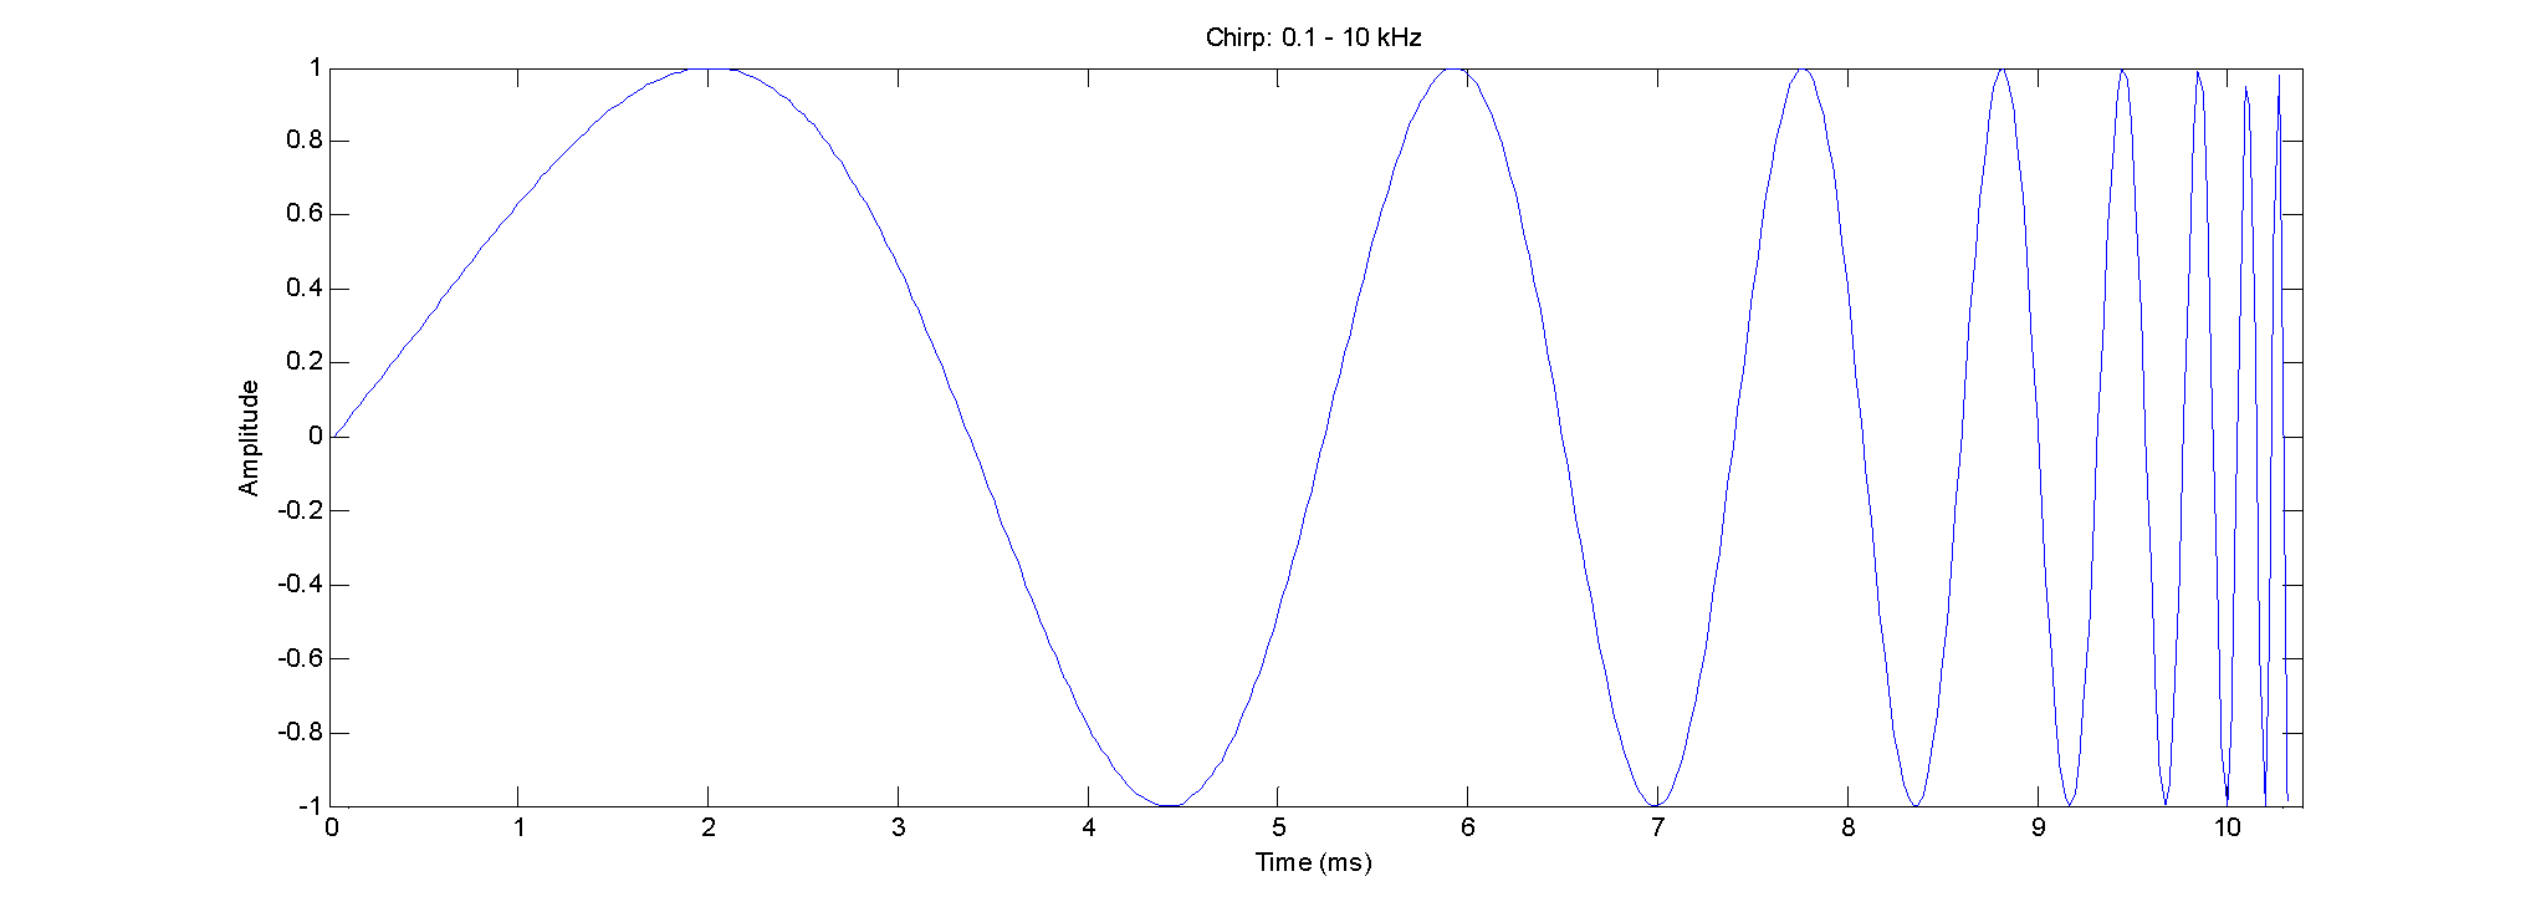
\includegraphics[width=1\textwidth]{images/Chirp.png}
  \caption{宽带Chirp信号(0.1 Hz 至 10 kHz)}
  \label{fig:ChirpfrequenceRange}
\end{figure}

\textbf{特定频率Chirp:}

除了用于全频段刺激的宽带 Chirp,本文也尝试使用频率有限的Chirp信号,称为频率特异性(Frequency-Specific)Chirps,来诱发ABR。Wegner 和 Dau(2002)发现,在低频(250 Hz)下,用一个以250 Hz为中心的 Chirp 刺激,比250 Hz的Tone刺激(Tone)产生更大的ABR响应幅度,尤其是在低到中等刺激强度下。
在本实验中使用的频率特异性 Chirp 波形具有以下特点:
频率范围约为一个倍频程(例如中心频率为500 Hz时,覆盖大约350-700 Hz);使用了高斯窗进行加窗,以控制其在时间域和频率域的形状。

\begin{figure}[H]
    \centering
    \begin{minipage}{0.48\textwidth}
        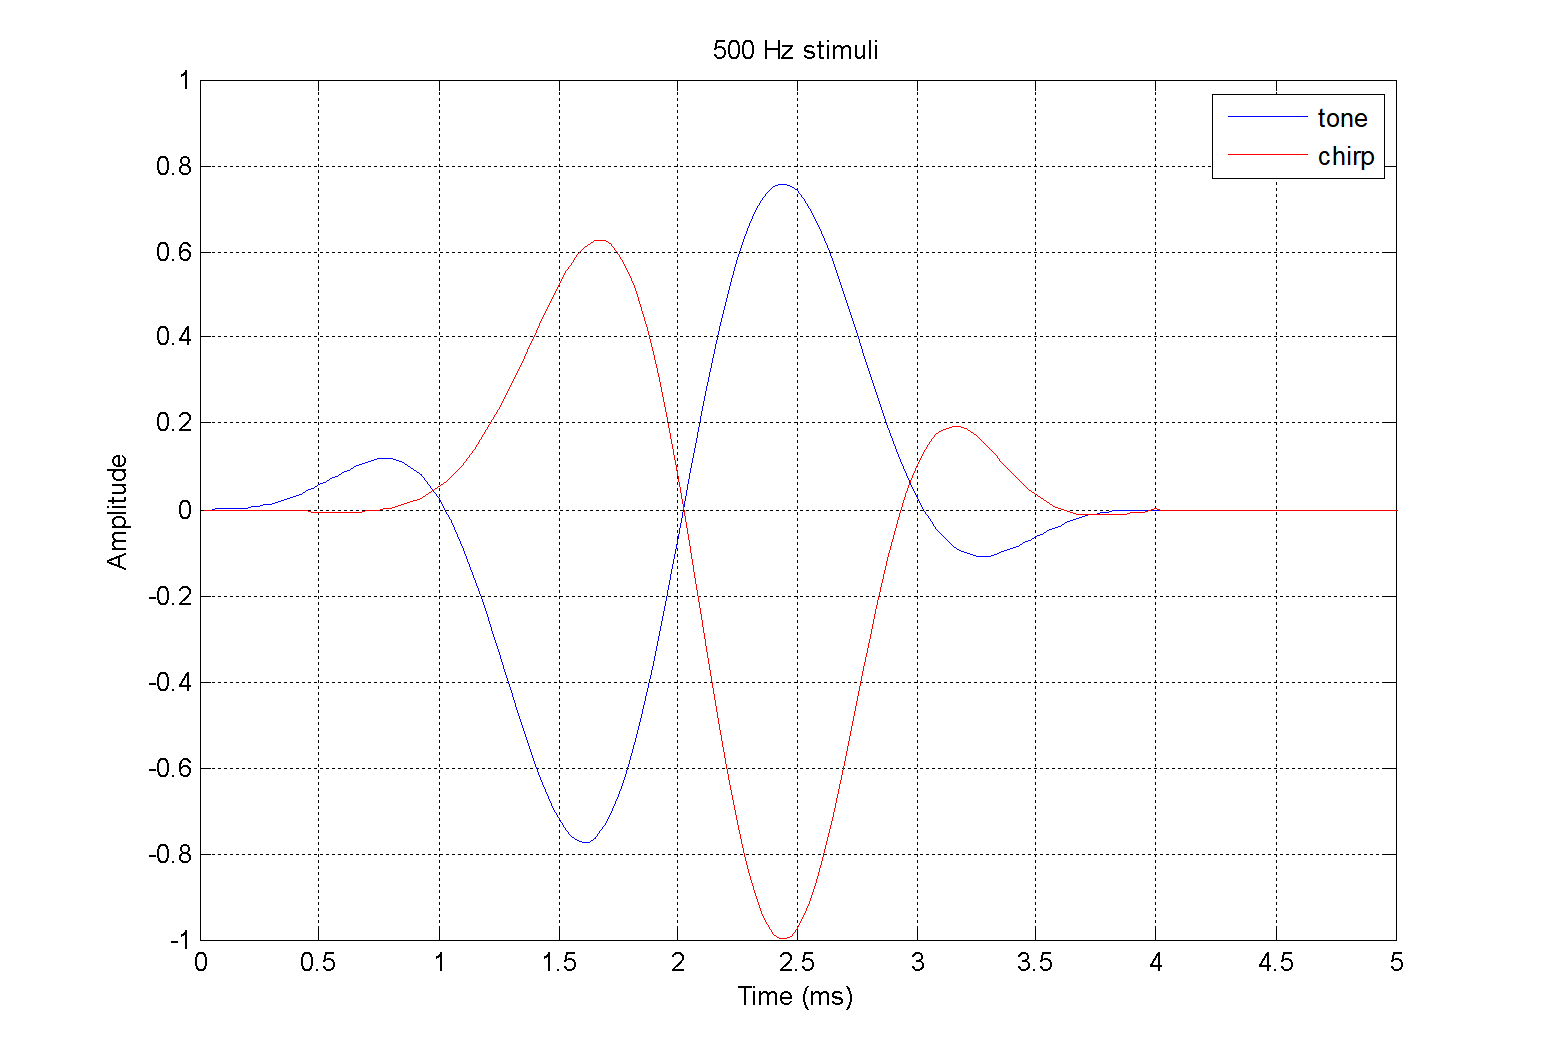
\includegraphics[width=\textwidth]{images/500hzStimuli.png}
    \end{minipage}
    \hfill
    \begin{minipage}{0.48\textwidth}
        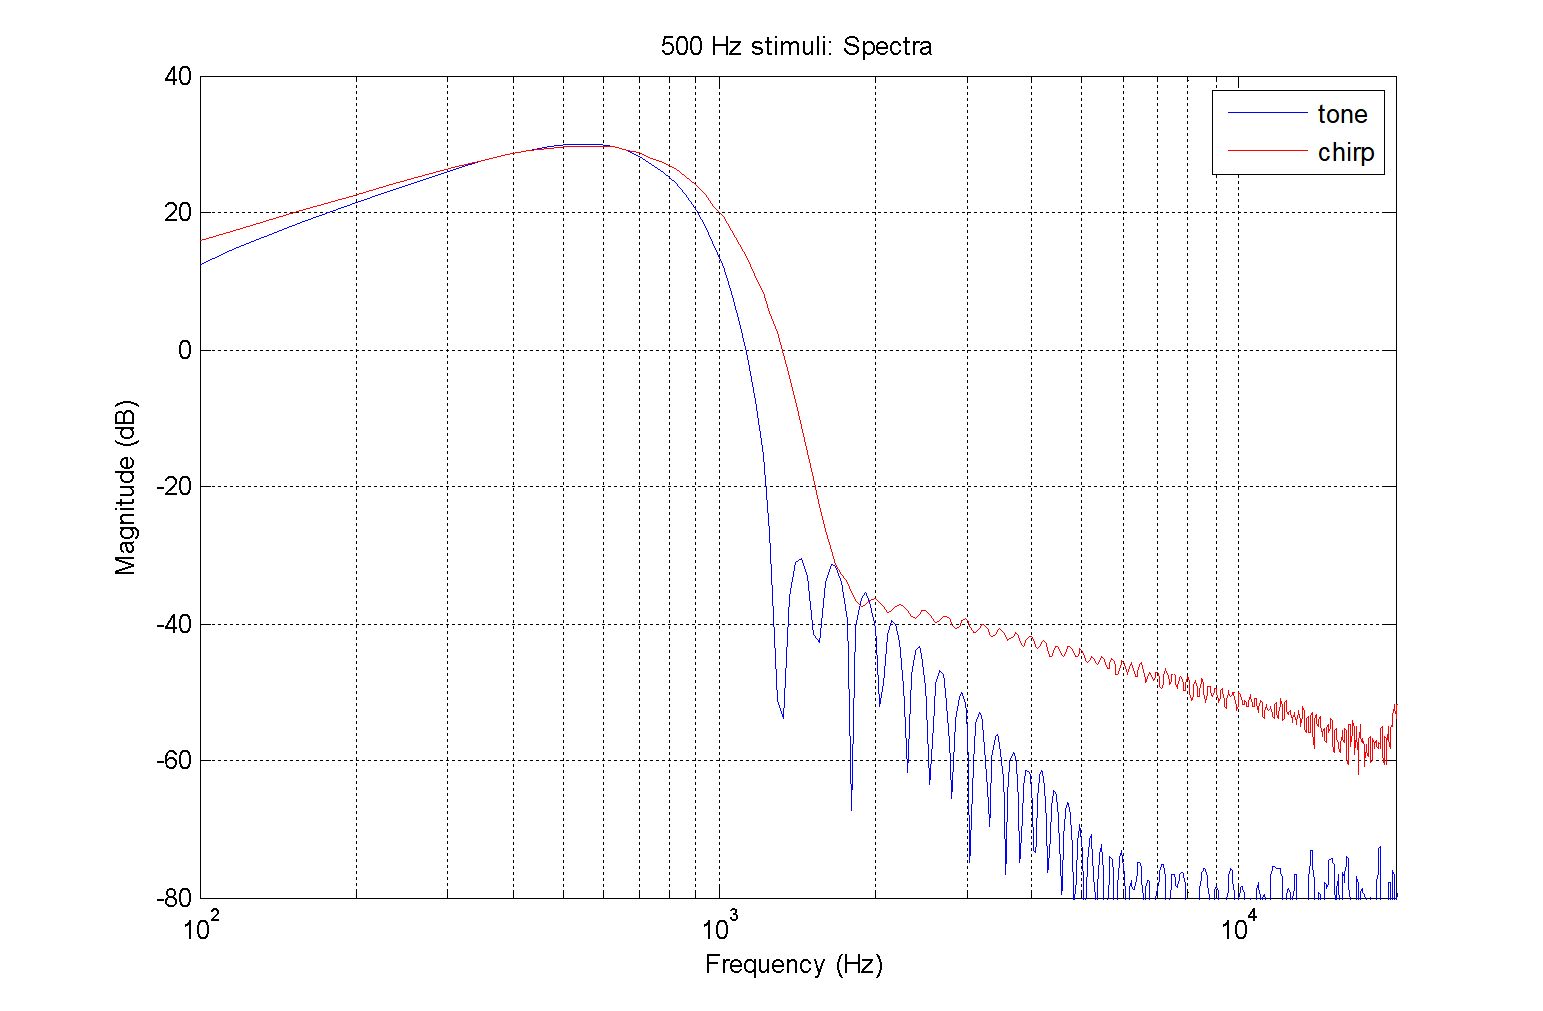
\includegraphics[width=\textwidth]{images/500hzSpectra.png}
    \end{minipage}
    
    \vspace{0.2cm}
    
    \begin{minipage}{0.48\textwidth}
        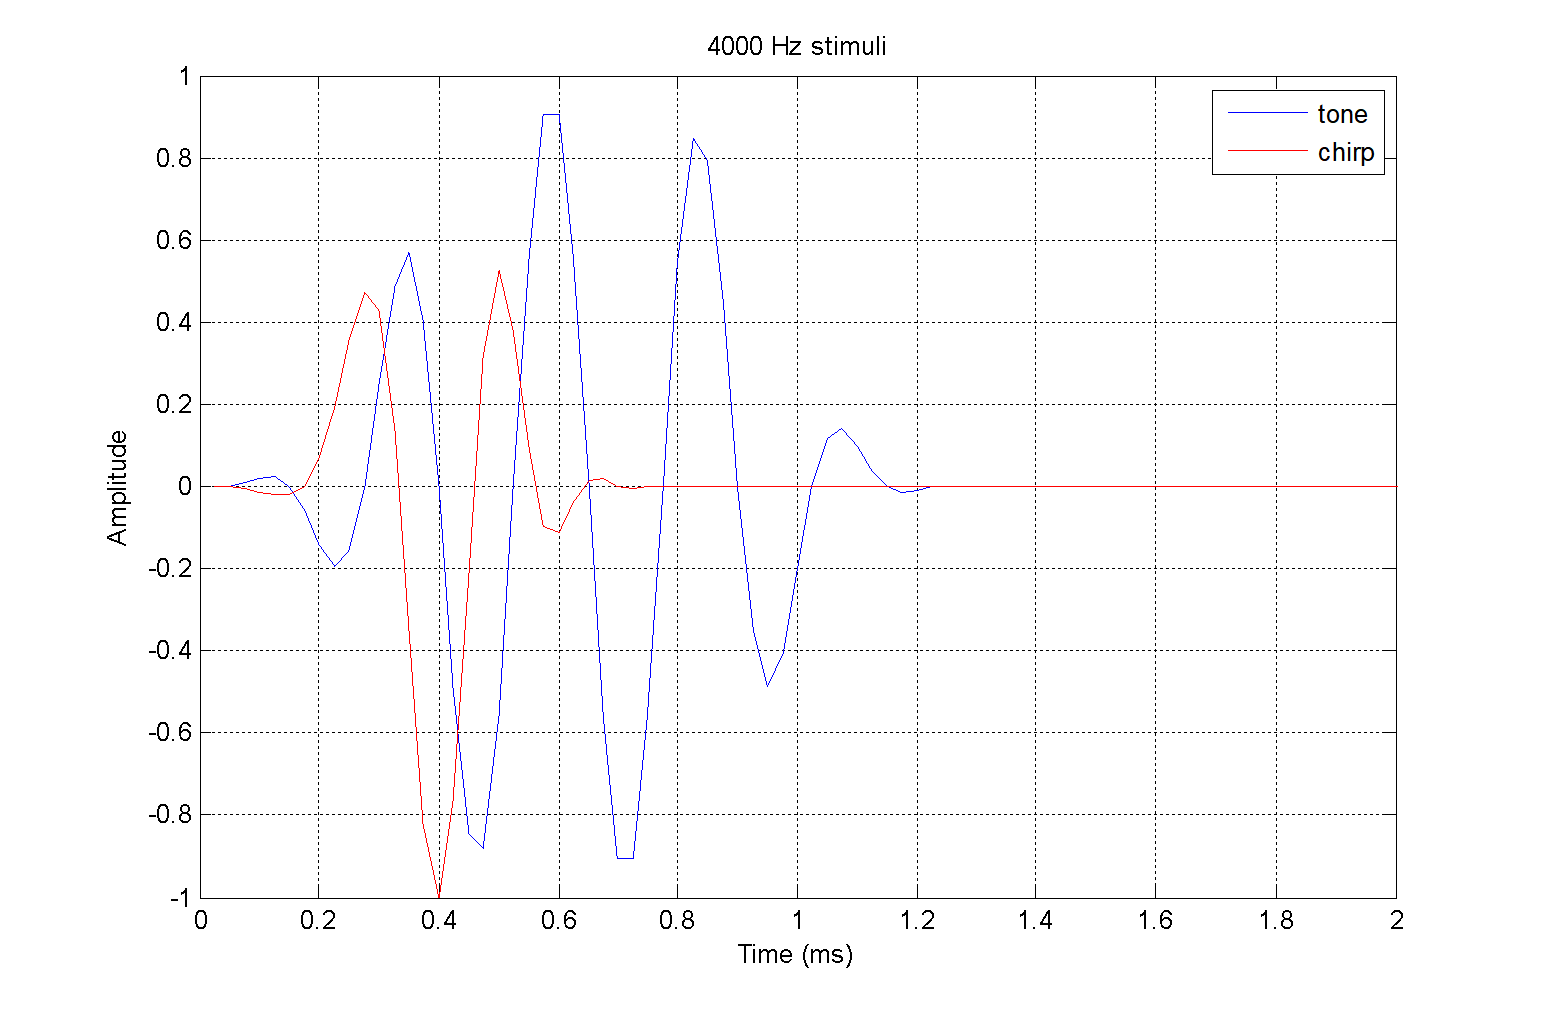
\includegraphics[width=\textwidth]{images/4000hzStimuli.png}
    \end{minipage}
    \hfill
    \begin{minipage}{0.48\textwidth}
        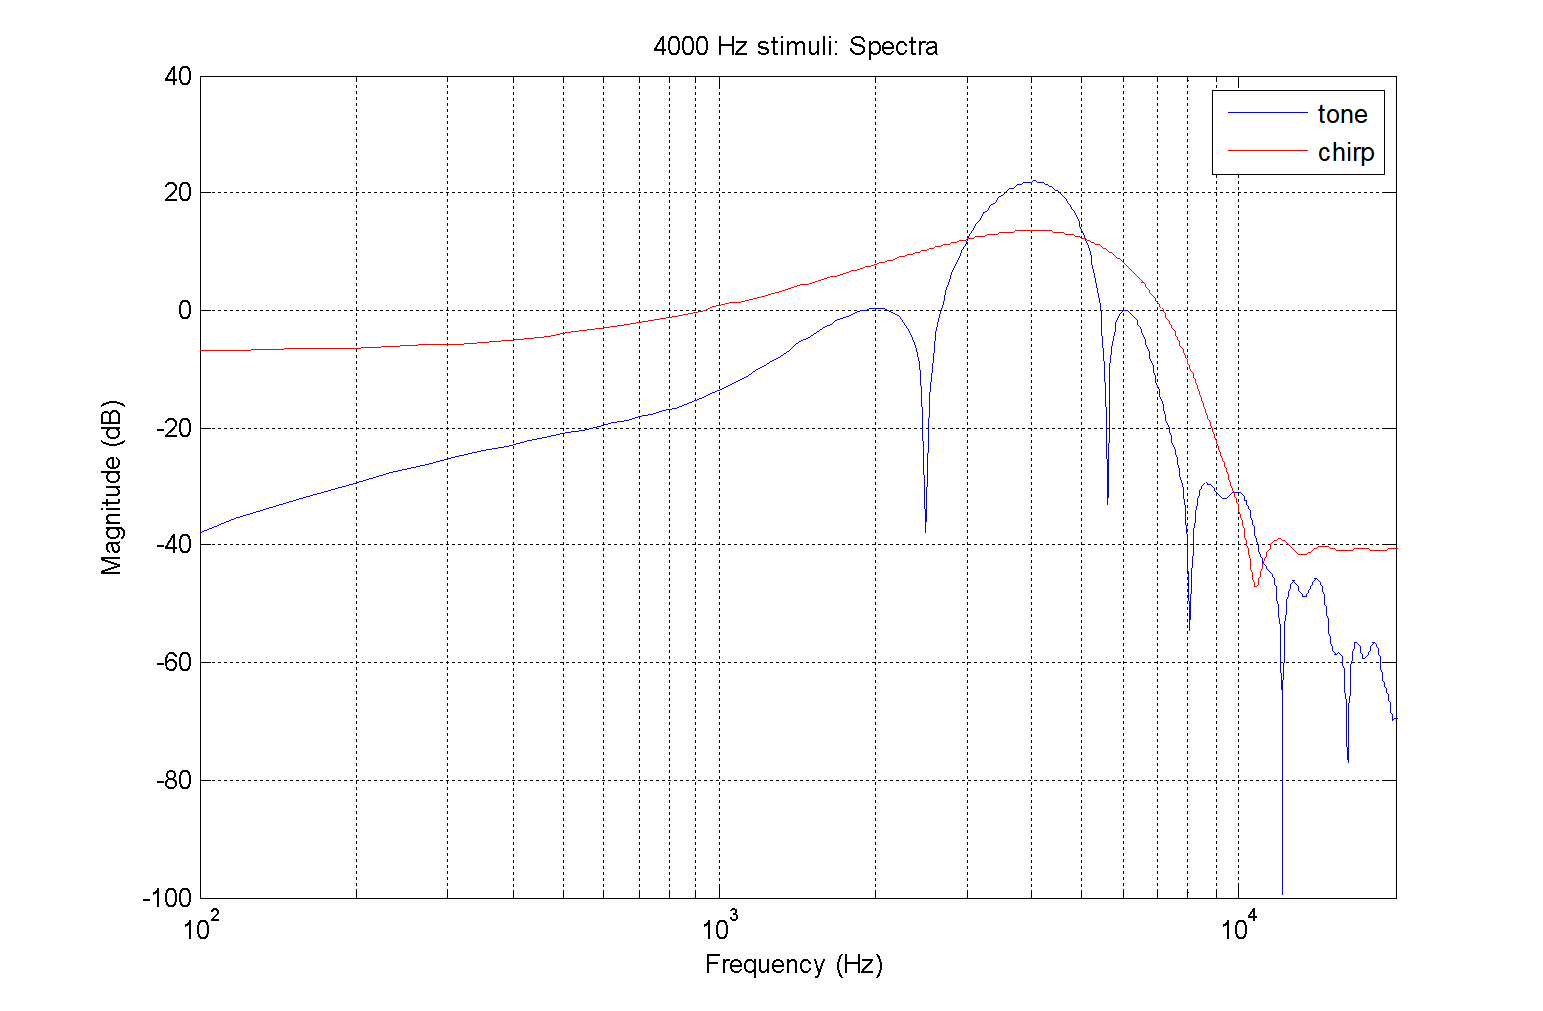
\includegraphics[width=\textwidth]{images/4000hzSpectra.png}
    \end{minipage}
    \caption{4 kHz、500 Hz的Tone和窄带Chirp刺激的时域波形与频谱图}
    \label{fig:4k500hzToneAndNarrowbandChirp}
\end{figure}
\FloatBarrier 
\section{优化刺激速率}

\textbf{交错频率:}
本研究精选了四个具有代表性的测试频率:4000Hz、2000Hz、1000Hz和500Hz。这些频率的选择基于以下考虑:

1)覆盖人类语音感知的关键频率范围;

2)代表耳蜗基底膜不同区域的特征响应; 

3)临床听力评估的标准测试频率点。

本设计的4频率设置既保证了足够的频率覆盖,又避免了过多频率导致的信号干扰问题。刺激间隔为18毫秒,音列之间的暂停时间为50毫秒。在无掩蔽噪声的条件下,交错频率序列中使用的单个Tone与单频刺激(每秒20个音爆)中使用的Tone完全一致。

\begin{figure}[H]
  \centering
  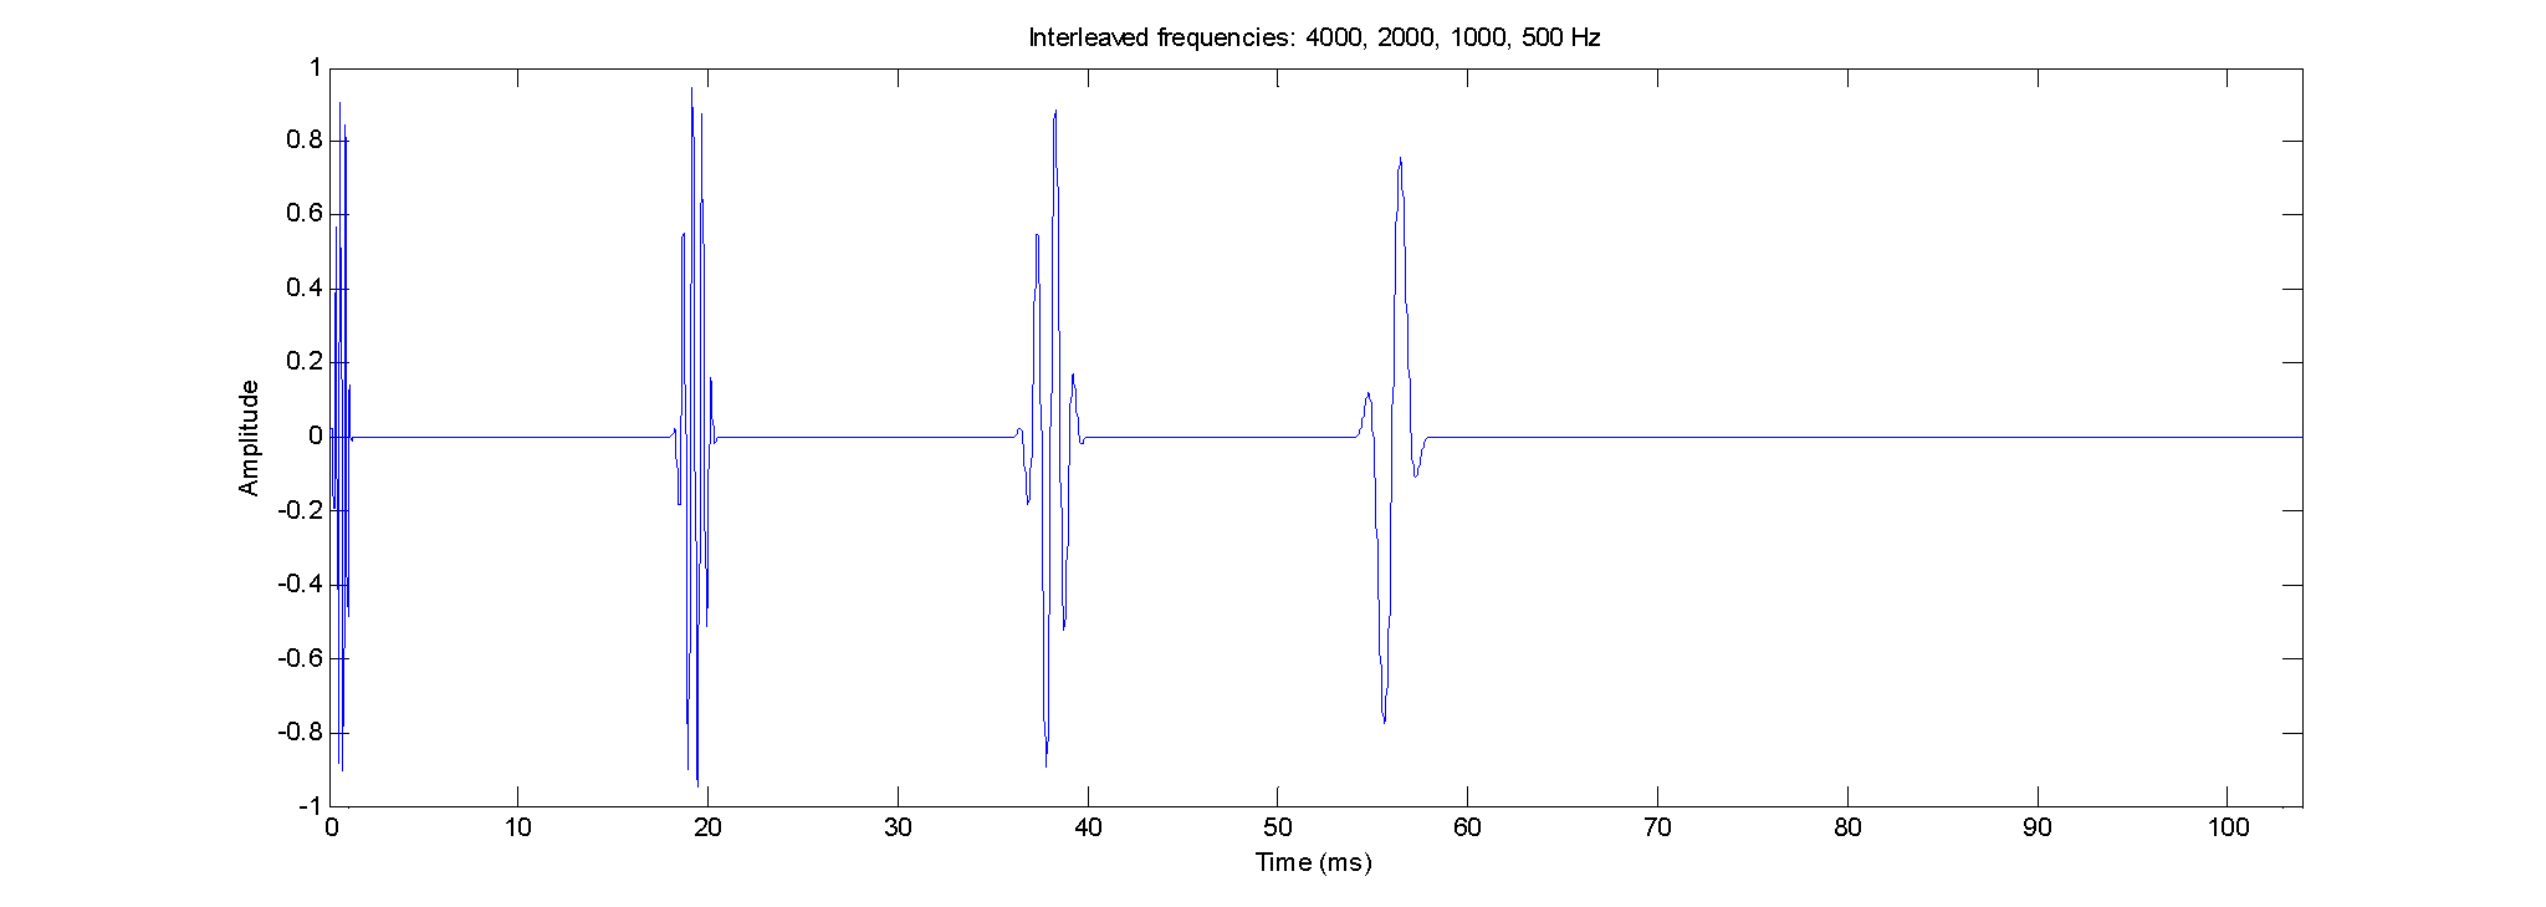
\includegraphics[width=1\textwidth]{images/InterleavedFrequencies.png}
  \caption{交错频率Tone的刺激序列}
  \label{fig:InterleavedFrequencies}
\end{figure}

\textbf{最大长度序列}

在传统刺激方式中,为避免响应之间的重叠,刺激速率通常受到神经反应持续时间的限制。使用最大长度序列(Maximum Length Sequence, MLS)可以显著提高刺激速率。MLS 是一种伪随机二进制序列,具有以下特殊自相关性质:其自相关函数在延迟为 0 时为序列长度 L,在其他任意延迟处均为 -1。这一特性使得即便多个刺激引发的神经反应重叠,仍可以通过反卷积将其有效分离。

在一个长度为 $L = 2^N - 1$ 的刺激序列中(其中 $N$ 为序列的阶数),共有 $2^N - 1$ 个点击声(Clicks)和 $2^N - 2$ 个静音间隔。该序列中有一半的脉冲之间的间隔为最小刺激间隔(Interstimulus Interval, ISI),其余的脉冲则以ISI的整数倍间隔分布。序列越长,ISI的变化也越大。

标准的 MLS 去卷积方法假设序列中所有刺激所诱发的反应是恒定的,然而实际上神经反应在高刺激速率下会发生适应性变化。具体而言:

\begin{enumerate}
    \item 随着刺激速率的增加,波形峰的潜伏期(Latency)会延长;而刺激强度越高,潜伏期越短;
    \item 随着刺激速率的增加,波形峰的幅度(Amplitude)会减小;而刺激强度越高,幅度会增加。
\end{enumerate}

由于不同ISI引起的反应幅度和潜伏期的变化,会导致在MLS反应的去卷积结果中出现未被抵消的波峰,从而增加了额外噪声。因此,在进行去卷积时,需要采用更复杂的非线性处理方法来解决这一问题。

\vspace{0.5em}
\noindent 其他需要考虑的因素包括:

\begin{itemize}
    \item \textbf{序列长度:} 序列过短时更容易被识别,也会在单位时间内重复出现更多次。若受试者能识别MLS序列的节奏,可能引发除单个刺激响应外的其他脑电反应。然而,序列越长,其ISI变化越大,反应波形的变异性也随之增加。本研究 ABR 试验中选择的序列长度为63(即MLS阶数为6)。
    
    \item \textbf{MLS速率:} 最优的MLS刺激速率(即在固定测试时间下获得最佳信噪比)与刺激强度有关。若仅考虑波V的检测,200~Hz 是超阈值条件下的最佳速率,而接近阈值时则以300~Hz表现最佳。本研究采用的刺激速率为250~Hz。
\end{itemize}

虽然MLS最常与Clicks一起使用,但也有研究探索了与Tone-Burst刺激及带限Chirp刺激的结合。

本研究中使用了中心频率为4~kHz和500~Hz的Tone-Burst刺激,以及以4~kHz和500~Hz为中心频率的窄带Chirp刺激。所用刺激序列的时域波形如图~\ref{fig:4k500hzToneAndNarrowbandChirp} 所示。

\begin{figure}[H]
    \centering
    \begin{minipage}{0.48\textwidth}
        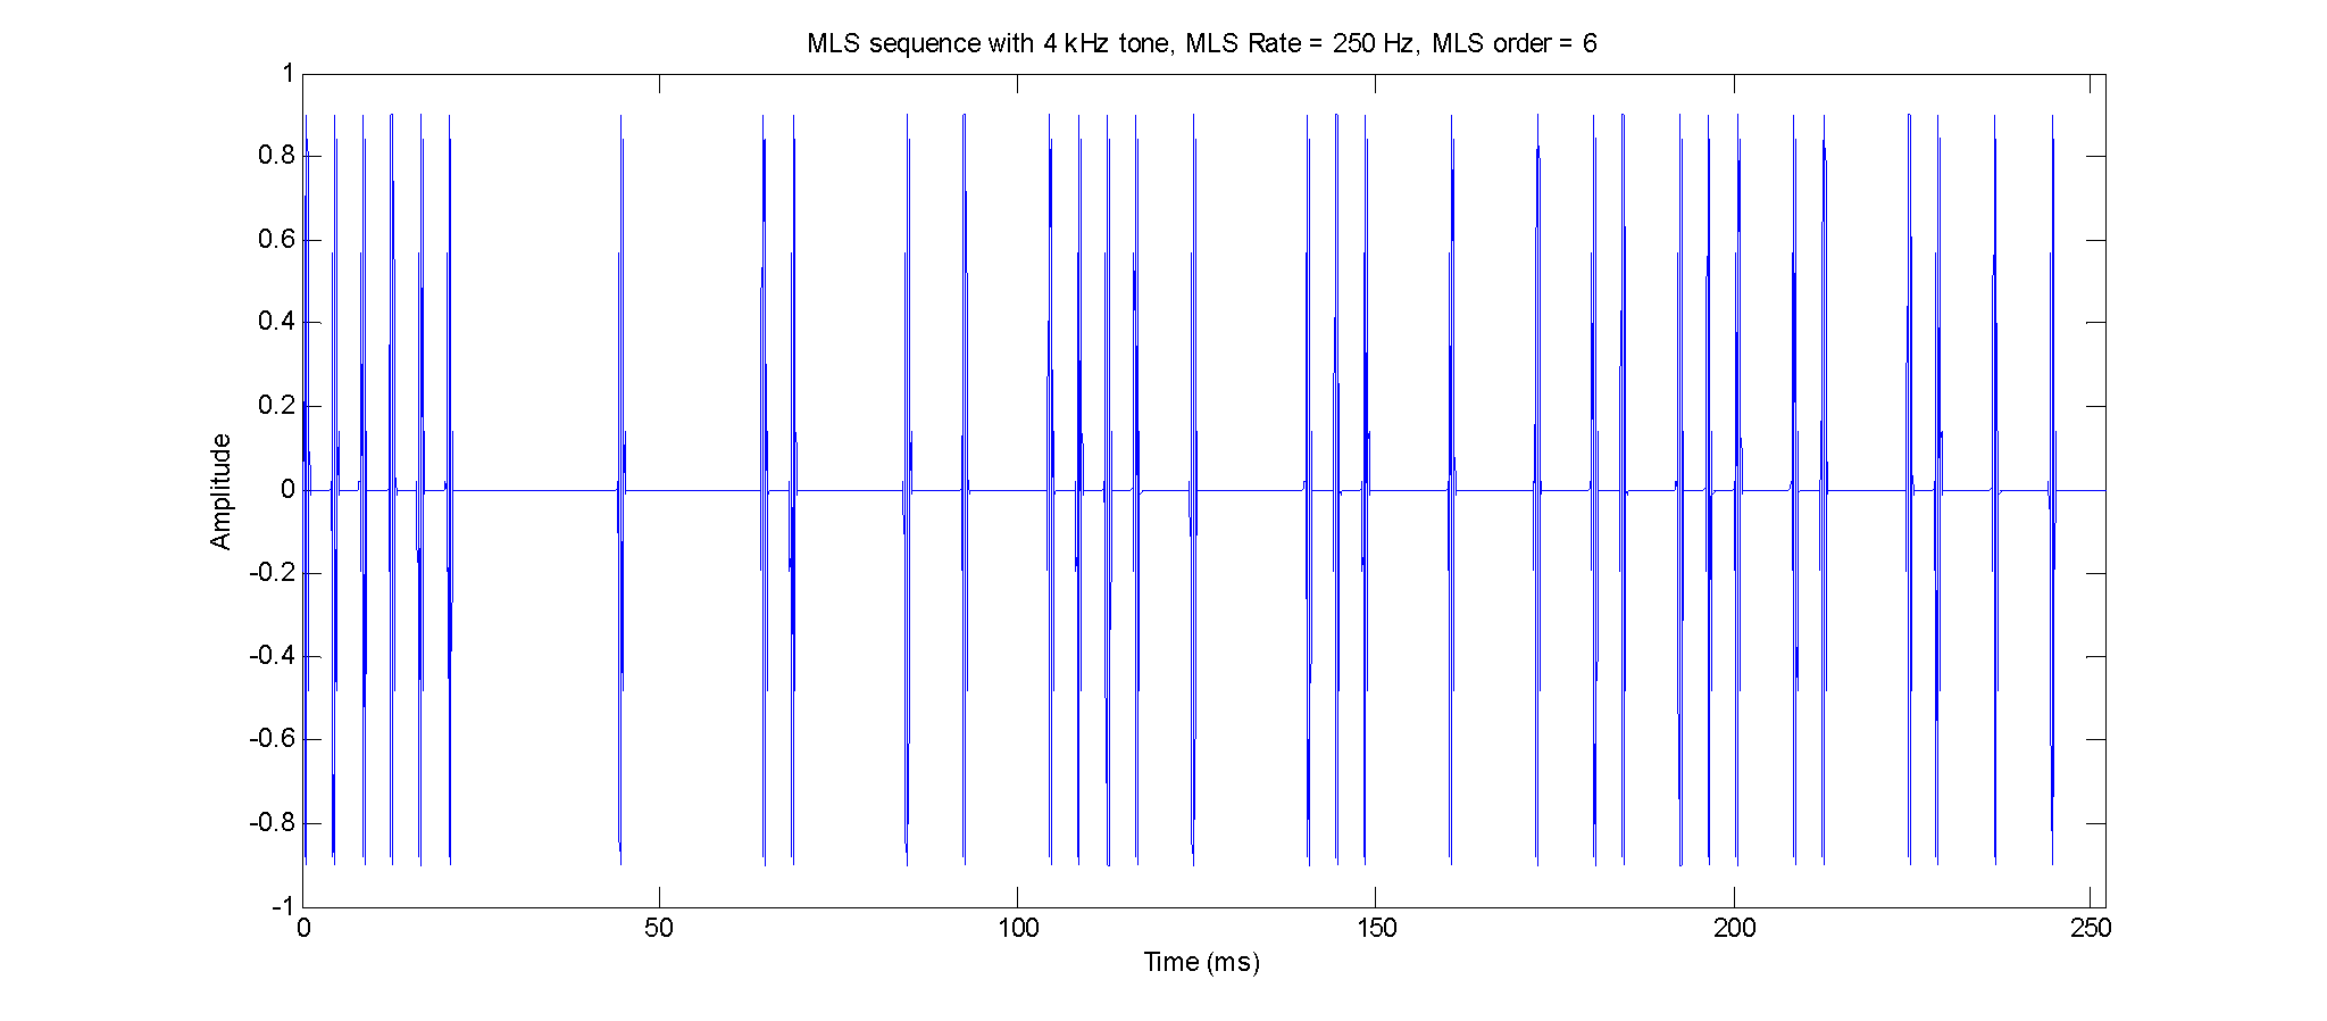
\includegraphics[width=\textwidth]{images/msl_sequence_with4kHztone.png}
    \end{minipage}
    \hfill
    \begin{minipage}{0.48\textwidth}
        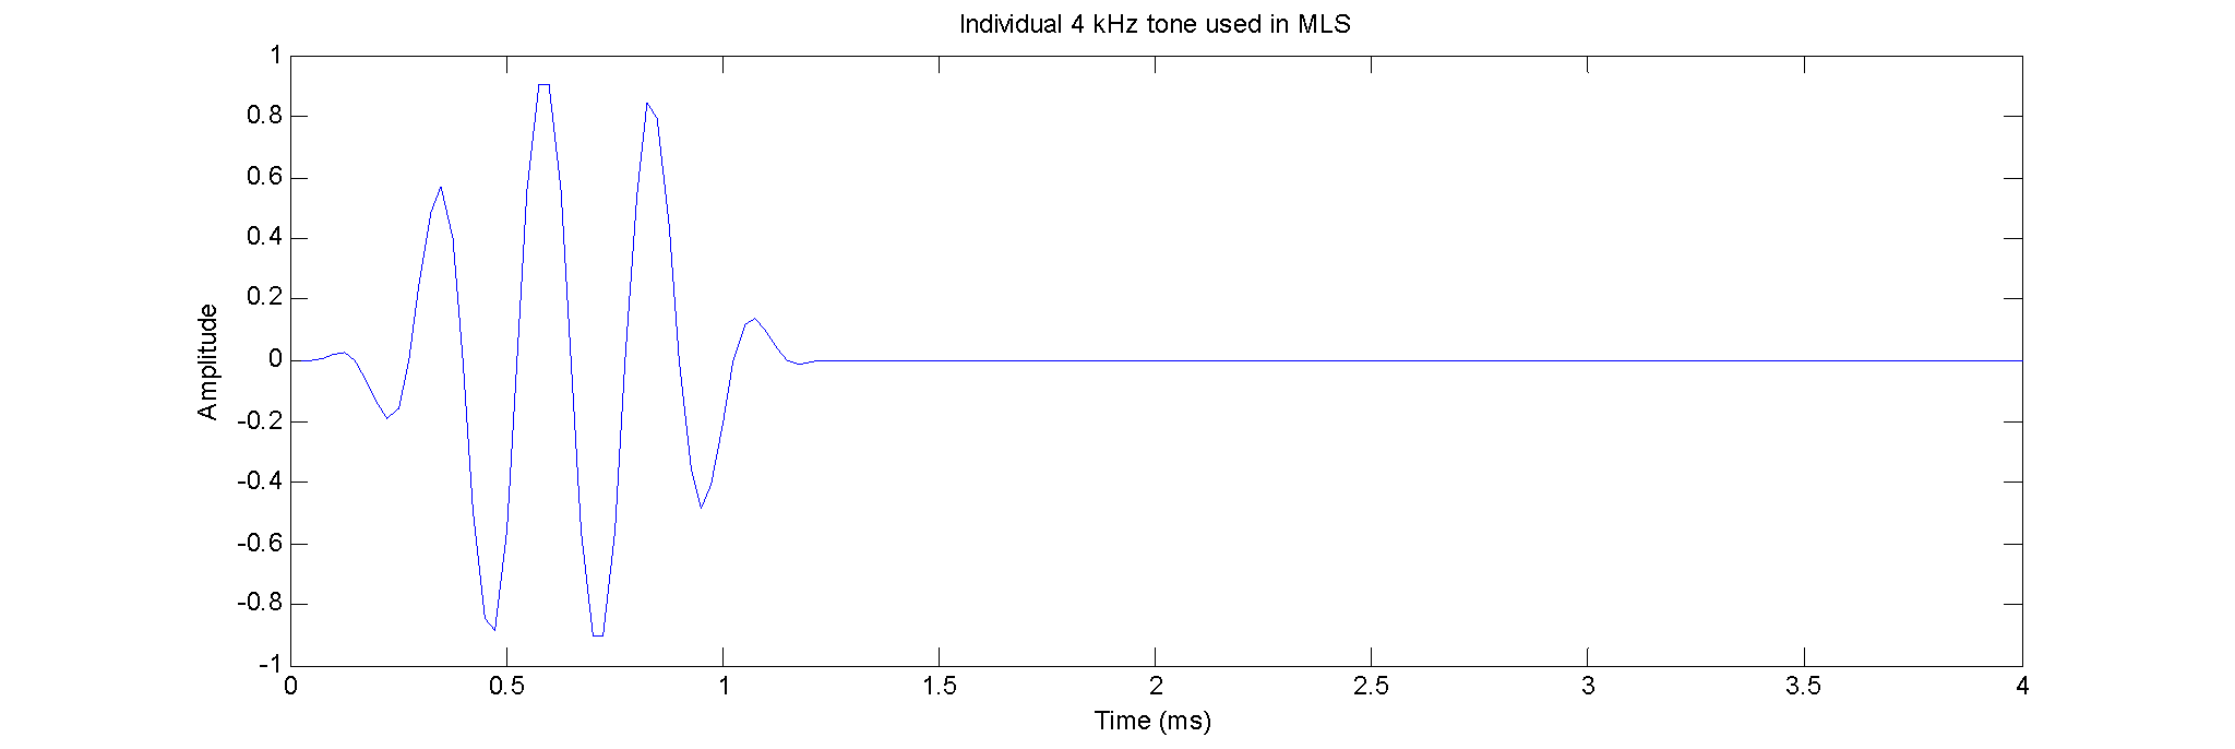
\includegraphics[width=\textwidth]{images/individual4kHzToneInMLS.png}
    \end{minipage}
    
    \vspace{0.2cm}
    
    \begin{minipage}{0.48\textwidth}
        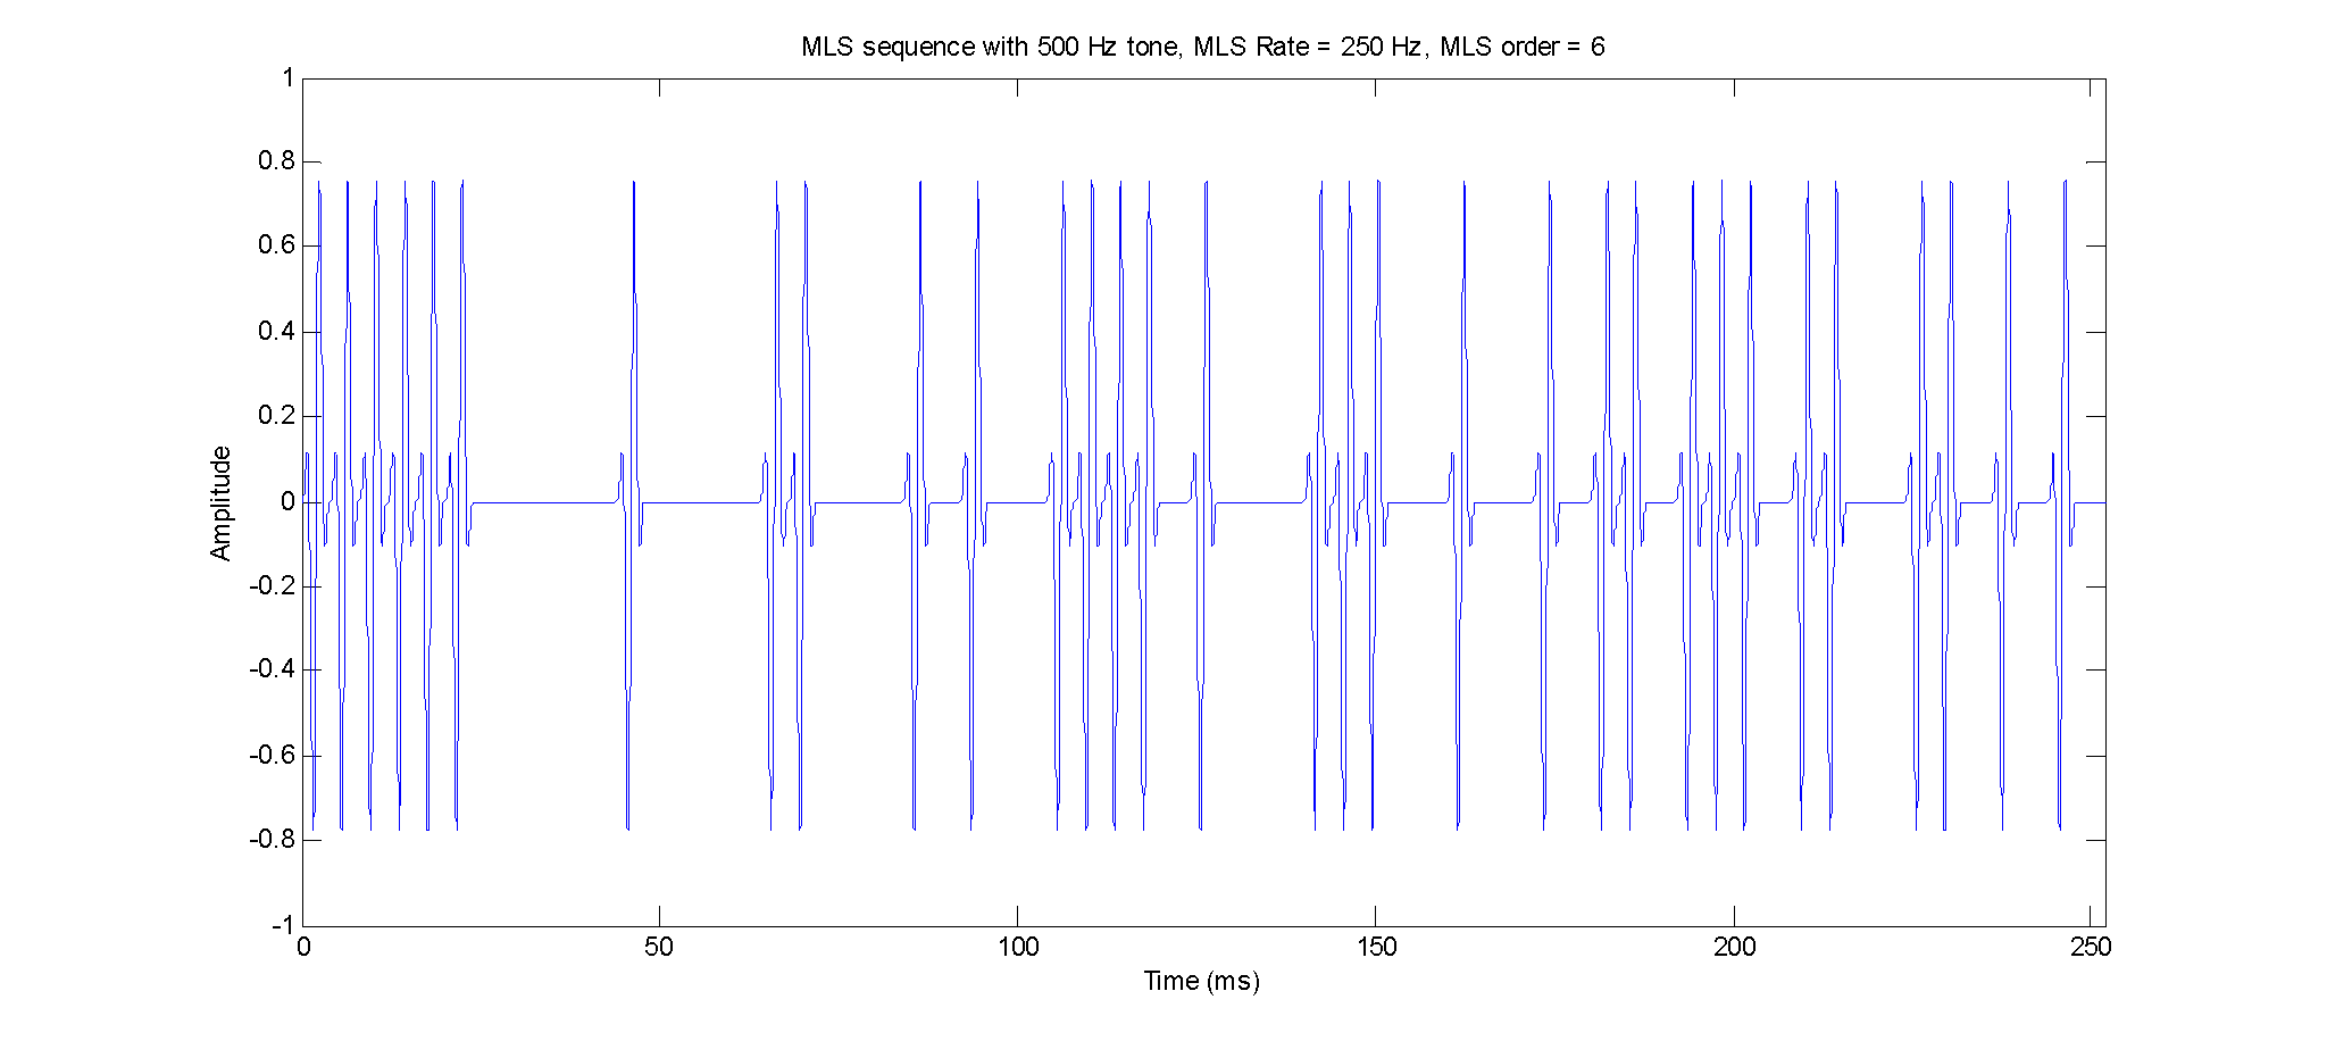
\includegraphics[width=\textwidth]{images/msl_sequence_with500Hztone.png}
    \end{minipage}
    \hfill
    \begin{minipage}{0.48\textwidth}
        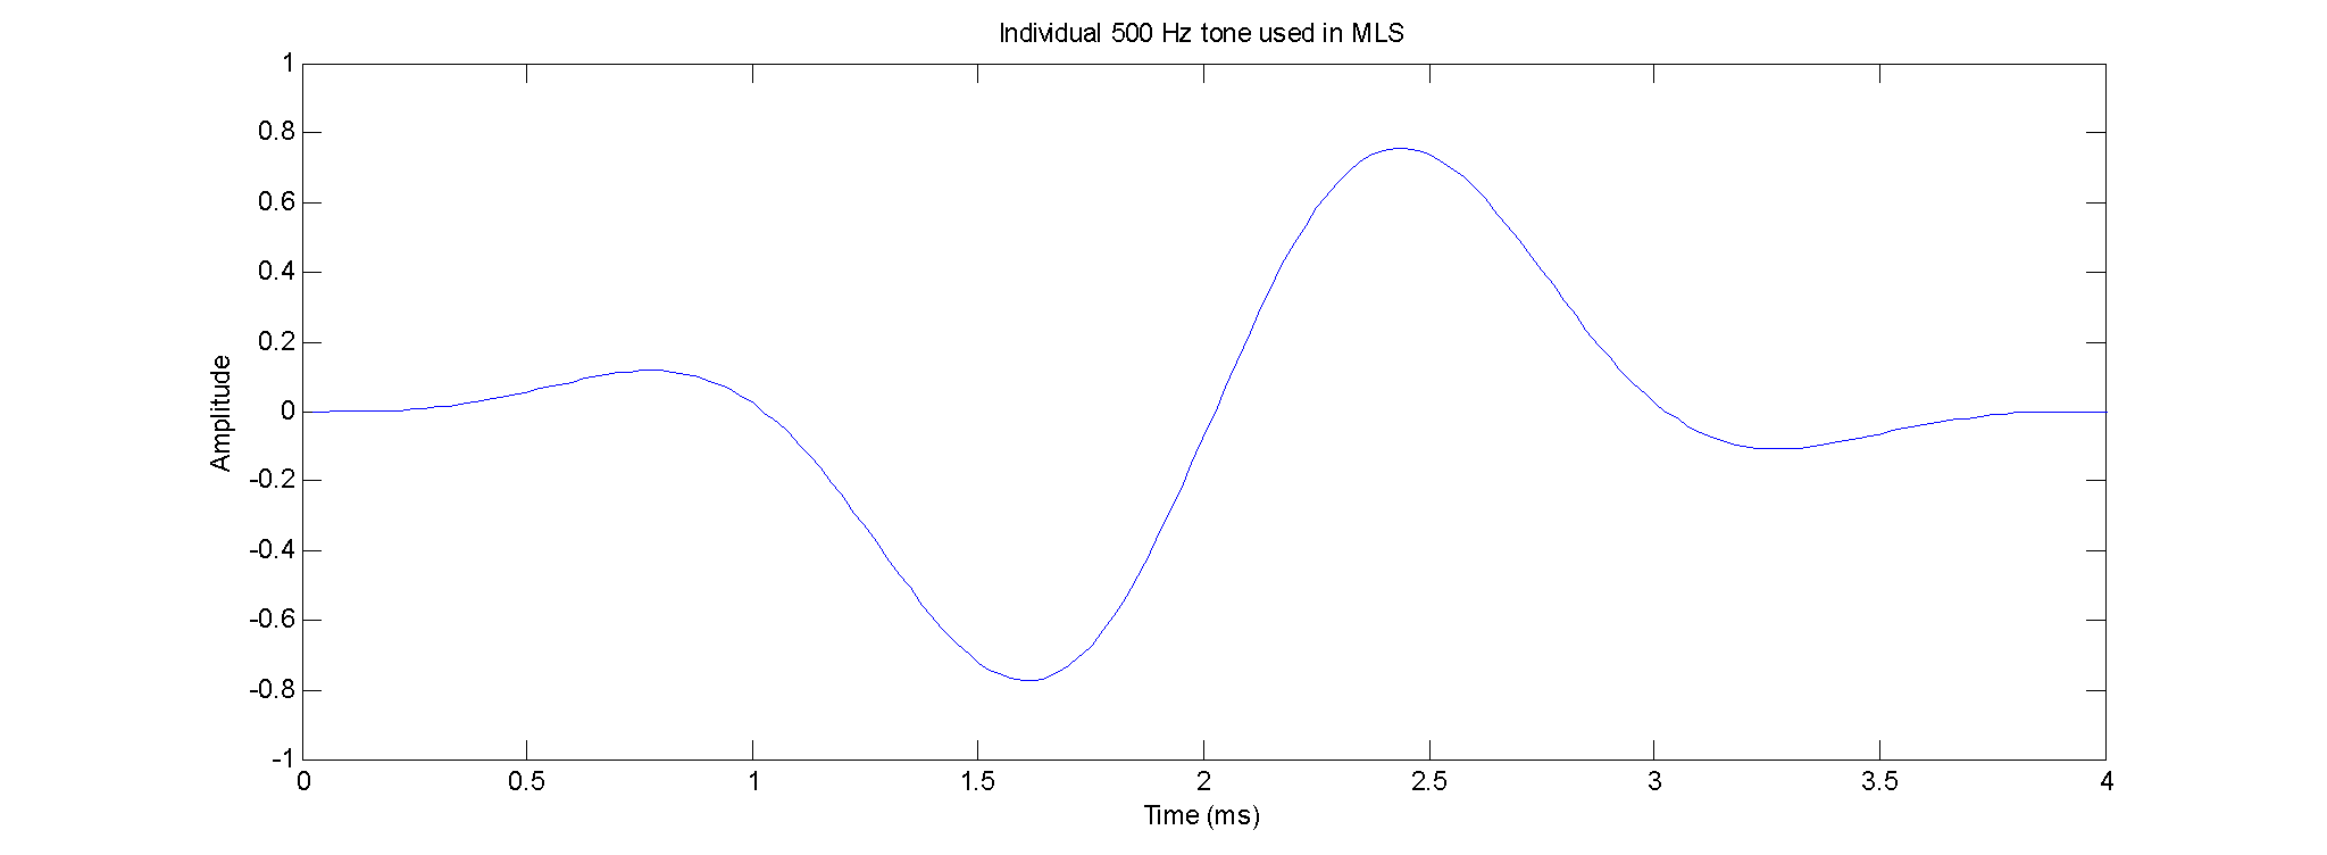
\includegraphics[width=\textwidth]{images/individual500HzToneInMLS.png}
    \end{minipage}
    \caption{4kHz、500HzTone的时域波形与频谱(MLS序列)}
    \label{fig:4k500hzToneAndNarrowbandChirp}
\end{figure}

\noindent \textbf{注意:}在500~Hz刺激中,采用了缩短的波形形式,以避免高频率刺激序列中出现的刺激重叠。这一配置不同于常规刺激中常用的2-0-2或2-1-2周期结构。


\section{改进的刺激与处理方法以降低噪声影响}
\subsection*{平均技术}

本研究中所有测试记录均应用了以下三种平均方法:
\paragraph*{普通平均}
时域集合平均(Time-domain ensemble averaging)是提高 SNR 最常见且基本的方法。假设 ABR 信号保持恒定且噪声为平稳噪声,平均 N 次后噪声贡献将按 $1/\sqrt{N}$ 的比例减小。在平均之前先进行滤波,以去除信号能量较少频段的背景噪声。本研究中使用的带通滤波器通带范围为 100–3000 Hz。
\[
\overline{X} = \frac{1}{N} \sum_{i=1}^{N} X_i
\]
\paragraph*{加权平均}
通常,背景噪声在整个记录过程中不会保持平稳,某些单次噪声爆发可能会显著影响平均结果的 SNR。对传统平均的一种改进是为每个扫掠分配一个基于该扫掠内噪声方差的权重因子,噪声越大的扫掠权重越低。其加权平均公式为:
\begin{align}
\overline{X_w} &= \frac{1}{C_N} \sum_{i=1}^N \frac{X_i}{V_i} \\
C_N &= \sum_{i=1}^N \frac{1}{V_i} \quad \text{(其中 } V_i \approx \frac{1}{N}\sum X_i^2 \text{)}
\end{align}

\paragraph*{区块加权平均}
该方法与加权平均类似,不同之处在于使用扫掠区块估计噪声方差。区块大小可为 10 至 250 次扫掠,较小区块尺寸更容易获取低噪声扫掠。这种方法也被称为贝叶斯加权。

加权平均优于伪迹拒绝(Artifact Rejection),因为它降低了噪声扫掠的影响,而无需事先设定拒绝阈值。

\subsection*{多通道噪声抑制}

多通道噪声抑制技术引入了额外电极,用于检测与主电极记录电压中噪声相关的信号。通过回归分析,计算两个通道之间的关系,从主通道信号中减去一个比例缩放后的辅助通道信号,从而获得降噪后的信号。

为了达到最佳效果,应将电极布置为:主通道信号强,辅助通道信号弱但与主通道噪声高度相关。与皮层反应不同,ABR 的 V 波在头皮多个区域都很强,尤其在对侧(Cz–A2)和水平阵列(A1–A2)上。

以下电极布置用于本研究:Cz – Inion、 Cz – Inion、 Cz – A1、  T1 – T2、 T1 – A1。
少数受试者也使用以下布置:Cz–A2、A1–A2、Shoulder–Inion。

\textbf{注意事项:}
\begin{itemize}
    \item Cz–Inion 相比 Cz–A1 记录到更大波幅的 V 波,但背景噪声也更高。
    \item T1–A1 的反应与 Cz–A1 类似。
    \item 不同电极布置在成人与婴儿间差异显著,新生儿常在同侧布置下获得良好 ABR,但在对侧布置下几乎无反应(Hall, 2007\cite{hall2007new})。
\end{itemize}

降噪处理的具体步骤如下:
\begin{equation}
    X_i' = X_i - a_i Y_i
\end{equation}
其中 $X_i$ 为信号通道每个时段的原始信号,$Y_i$ 为辅助通道信号,$a_i$ 为缩放因子,其通过最小化调整信号的导数功率来计算:
比例因子$a_i$通过最小化信号功率求得:
\[ S = \sum_j (X_{i,j} - a_i Y_{i,j})^2 \]
\[ \frac{\partial S}{\partial a_i} =  \sum_j -2Y_{i,j}(X_{i,j} - a_i Y_{i,j}) = 0 \]

最终解:
\[ a_i = \frac{\sum_j X_{i,j} Y_{i,j}}{\sum_j Y_{i,j}^2} \]
其中 $j$ 表示刺激后 4–14 ms 内所有采样点。最终得到的平均降噪信号 $\bar{X}'$ 应保留原始 ABR 的峰值幅度,同时背景噪声更低,从而提高信噪比。

\subsection*{自适应滤波}
自适应滤波通过动态调整频率响应,在 SNR 最差的频段降低增益,可有效抑制噪声时段或特定频段的干扰。加权平均是自适应滤波的特例,其根据响应区间的噪声水平进行反向加权。

\subsubsection{时变滤波方法(1)}
滤波器响应设计为:
\[
G(f) = \frac{|S(f)|^2}{|S(f)|^2 + |N(f)|^2} \approx \frac{|S(f)|^2}{|N(f)|^2}
\]
\begin{itemize}
\item $S(f)$:由平均ABR波形或原型波形估计
\item $N(f)$:由单次扫描频谱(主要含背景噪声)估计
\end{itemize}
滤波器系数定期更新(如每次扫描),通过实时滤波降低背景噪声。

\subsubsection{时变滤波方法(2)}
基于Wiener滤波的单通道降噪模型:
\begin{figure}[H]
  \centering
  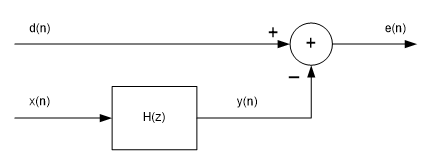
\includegraphics[width=0.5\textwidth]{images/wienerfiltering.png}
  \caption{维纳滤波噪声抑制系统框图}
  \label{fig:InterleavedFrequencies}
\end{figure}
\begin{itemize}
\item[$\bullet$] \textbf{输入信号}:含噪时段信号$x(n)$作为系统主输入
\item[$\bullet$] \textbf{期望信号}:$d_i(t)$通过排除第$i$时段的所有时段平均构建,以满足输入信号与期望信号不相关假设
\end{itemize}
\[ 
d_i(n) = \frac{1}{P} \sum_{\substack{j=0 \\ j \neq i}}^{P} x_j(n) 
\]
滤波器输出
\[ y_i(t) = \sum_{m=0}^{M-1} h_i(m)x_i(t-m) \]
其中 $h_i(m)$ 表示滤波器的冲激响应,其通过最小化误差信号的均方值求得:
这里误差信号 $e_i(n)$ 定义为:
\[
e_i(n) = d_i(n) - y_i(n)
\]
最优冲激响应是维纳-霍夫方程的解,其表达式为:
\[
\sum_{m=0}^{M-1} h_i(m) r_{x_i}(m-k) = p(-k), \quad k = 0,1,...,M-1
\]
其中:
\begin{itemize}
\item $r_{x_i}(m-k)$ 是输入信号的自相关函数
\item $p(-k)$ 是输入信号与期望信号的互相关函数
\end{itemize}

当噪声与目标信号的频谱重叠较小时,该方法效果最佳。
\subsection*{主成分分析与独立成分分析}
主成分分析(PCA)和独立成分分析(ICA)是两种信号处理方法,其目的是将波形分解为多个分量,并消除主要由噪声源产生的分量。
在PCA中,需要计算数据协方差矩阵的特征向量和特征值。对于n维数据集(n为ABR时间窗内的时间采样点数),共有n个特征向量。前几个分量包含信号的大部分方差,具有最大特征值的特征向量即为主成分。可根据特征值大小选择特征向量子集来重建信号。

ICA主要用于多通道分析,常用于处理EEG数据。若存在n个源信号,至少需要n个观测通道(即n个通道)才能获取原始信号。给定一组测量信号(即独立信号的混合),ICA通过变换产生具有最大非高斯性的独立分量信号。数据分解过程涉及从单通道头皮采集数据到空间变换"虚拟通道"基的线性转换。也就是说,数据从多个同步记录的单通道数据集合,转换为应用于整个多通道数据的空间滤波器的同步输出集合。
ICA将$n$维多元时间序列$\mathbf{x}$建模为$M$($M \leq n$)个统计独立源的线性组合。


给定$n$个线性混合信号和$n$个源信号:
\begin{itemize}
    \item 观测信号:$X_1, X_2, \ldots, X_n$
    \item 源信号:$S_1, S_2, \ldots, S_n$
\end{itemize}

\noindent 混合过程表示为:
\[
X_j = \sum_{k=1}^n a_{j,k}S_k \quad \text{其中}\; j = 1,2,\ldots,n
\]

\noindent 矩阵形式:
\begin{align*}
\mathbf{x} &= \mathbf{A}\mathbf{s} \quad \text{(混合方程)} \\
\mathbf{s} &= \mathbf{A}^{-1}\mathbf{x} = \mathbf{W}\mathbf{x} \quad \text{(分离方程)}
\end{align*}
\section{自动检测方法}
\subsection*{Hotelling's T²}
Hotelling's T²统计量用于多元假设检验。在“不存在响应信号”的零假设条件下,该方法通过计算数据样本任意线性组合的均值与零的显著性差异概率来进行统计推断。

在ABR检测中的具体应用步骤如下:首先对信号进行1500Hz低通滤波预处理;随后将感兴趣信号区域划分为10个时间仓(每个仓宽0.45ms)——对于75dB感觉级刺激的响应从5.5ms开始分段,40 dB 感觉级刺激则从8.5ms开始;接着计算各时间仓内的信号平均值;最终每个时段提取10个特征点作为T²分析的输入数据。
\[
T^2 = N(\bar{\mathbf{x}} - \boldsymbol{\mu})^\top \mathbf{S}^{-1}(\bar{\mathbf{x}} - \boldsymbol{\mu})
\]

其中:
\begin{itemize}
    \item $N$:扫描次数
    \item $\bar{\mathbf{x}}$:平均数据向量
    \item $\boldsymbol{\mu}$:零假设下的总体均值向量(本文中$\boldsymbol{\mu} = \mathbf{0}$)
    \item $\mathbf{S}$:$p \times p$维数据协方差矩阵
\end{itemize}

T$^2$统计量可通过以下关系转换为F分布:
\[
\frac{(N - p)T^2}{(N - 1)p} \approx F_{(p, N - p)}
\]
因此,可以确定存在响应信号的概率。
\subsection*{F$_{sp}$方差比}
F$_{sp}$方差比是检测 ABR 信号的标准方法,尤其适用于新生儿听力筛查。该指标通过计算以下方差比实现:

\[
\text{F}_{sp} = \frac{\sigma^2_{\text{信号}}}{\sigma^2_{\text{噪声}}}
= \frac{\mathrm{var}(\overline{X})}{\mathrm{var}(SP)}
\]
\[
\mathrm{var}(\overline{SP}) = \frac{\mathrm{var}(SP)}{N}
\]

\begin{itemize}
    \item \textbf{分子}:多次扫描平均波形的幅值方差
    \item \textbf{分母}:固定时间点处各扫描幅值的方差
\end{itemize}
翻译如下:

用于计算 F$_{sp}$ 的时间窗口的大小和位置可以根据刺激类型、呈现强度以及感兴趣波形特征的潜伏期进行调整。基于获得的 ABR 记录数据,以及主要关注的是检测 V–V' 波的存在与否,因此 F$_{sp}$的计算可以使用一个以 V 波为中心的较短时间窗口。在本研究中,使用的时间窗口为刺激后 7–11 毫秒(对应 75 dB SL)或 8–12 毫秒(对应 40 dB SL)。

 F$_{sp}$  与信噪比之间的关系如下:
\[
F_{SP} = \left[ SNR^2 + 1 + 2 \cdot R(EP, \overline{BN}) \cdot SNR \right] \cdot \frac{\mathrm{var}(\overline{BN})}{\mathrm{var}(\overline{SP})}
\]
方差比遵循 $F$ 分布 \( F(v_1, v_2) \),其中 \( v_1 \) 和 \( v_2 \) 分别是分子和分母的自由度。如果背景噪声是真正的白噪声,那么自由度 \( v_1 \) 应等于时间窗内的采样点数。然而,噪声的带宽越窄,自由度 \( v_1 \) 越低,因此该值需要进行估计。本文使用了一个非常保守的估计,即 \( v_1 = 5 \)。

分母的自由度 \( v_2 \) 是试次数 \( N \)。

根据 $F$ 分布查找表 \( F_{(5, 250)} \),95\% 置信水平的阈值为 2.25,99\% 置信水平的阈值为 3.1。在新生儿听力筛查中,通常使用F$_{sp}$ 值为 3.1 作为通过/未通过的判定标准。

由于在样本量较小的情况下,单点方差并不能准确估计背景噪声的方差,因此在本研究中, F$_{sp}$  比值的分母是基于时间窗内全部 \( J \) 个采样点所计算的方差,并对结果进行了平均处理。
\[
F_{SP} = \frac{\text{var}(S)}{\frac{1}{J}\sum_{j=1}^{J}\text{var}(\overline{SP}_{j})}
\]
\subsection*{方差比点(POVR)}
POVR与  F$_{sp}$ 类似,但其分子部分的方差更大,因为仅使用响应中的部分时间点(如4或10个点),而非全部数据点(Sininger等,2001)。所选时间点通过最大化目标/模板波形的方差来确定,通常包括目标波形的最大峰值和最小峰值(对于ABR,可能是波III、波V或波V')。

由于波形形态会因刺激类型、速率、呈现强度、电极位置和受试者年龄等因素而变化,可以预见,不同刺激条件下可能需要不同的模板或时间点。此外,若个体存在峰值潜伏期偏移,检测功效也会降低。

\section{实验与结果}
\subsection*{刺激集}
呈现的完整刺激集包括:
\begin{table}[H]
\centering
\caption{听觉刺激参数表}
\label{tab:stimulus_params}
\begin{tabular}{llll}
\toprule
\textbf{刺激类型} & \textbf{极性/频率} & \textbf{呈现速率} & \textbf{强度(dB SL)} \\
\midrule
\hline
Click & 稀疏(Rarefaction) & 10, 20 Hz & 75, 40 \\
     & 凝聚(Condensation) &          &   \\
\hline
单调音(Tone) & 4000 Hz  &       & 75, 40 \\
            & 500 Hz              &       & \\
            & 500 Hz(交替极性)    &       & 75, 40 \\
\hline
M-Chirp & 100–10400 Hz & 20 Hz & 75, 40 \\
\hline
Octave Chirp & 4000 Hz &       &           \\
                      & 500 Hz  &       &           \\
\hline
\multirow{5}{*}{MLS} & Click        & 250 Hz, 300 Hz & 75, 40 \\
                                   & 500 Hz Tone   & 250 Hz         & 75, 40 \\
                                   & 4000 Hz Tone  &   &  \\
                                   & 500 Hz Chirp   &    &  \\
                                   & 4000 Hz Chirp  &    &  \\
\hline
交错频率 & Tone4k,2k,1k,500Hz& Tone18ms,序列55ms & 75, 40 \\
        & Chirp4k,2k,1k,500Hz& &    \\
\hline
GHINOMA & Tone4k,2k,1k,500Hz&       & 65 \\
        & Chirp4000,2000,1000,500Hz &       &   \\
\bottomrule
\end{tabular}
\end{table}

\subsection*{实验设置}
Neuroscan EEG系统是专业脑电采集平台,广泛应用于临床神经生理学和认知神经科学研究。系统以高精度信号采集和灵活的配置著称,支持从常规脑电到事件相关电位(ERP)的全方位研究需求。

\begin{figure}[H]
\centering
% 左表格:系统参数
\begin{minipage}[t]{0.48\textwidth}
\centering
\captionof{table}{系统硬件参数} % 添加的标题
\adjustbox{valign=t}{
\begin{tabular}{>{\bfseries}ll}
\toprule
\textbf{参数} & \textbf{设置值} \\
\midrule
A/D采样率 & 20,000 Hz \\
增益 & 2500 \\
高通滤波 & 100 Hz \\
低通滤波 & 3000 Hz \\
采样模式 & Continuous \\
伪迹剔除阈值 & ±50 μV \\ % 补充单位说明
\bottomrule
\end{tabular}
}
\label{tab:hardware_params}
\end{minipage}
\hfill
% 右表格:电极配置
\begin{minipage}[t]{0.48\textwidth}
\centering
\captionof{table}{电极配置方案} % 添加的标题
\adjustbox{valign=t}{
\begin{tabular}{>{\bfseries}l>{\ttfamily}l}
\toprule
\textbf{通道} & \textbf{导联设置(电极位置)} \\ % 修改列名
\midrule
通道1 & Cz → Inion (顶点→枕骨隆突) \\
通道2 & Cz → A1 (顶点→左耳垂) \\
通道3 & T1 → T2 (左颞→右颞) \\ % 统一缩写
通道4 & T1 → A1 (左颞→左耳垂) \\ % 补充说明
\addlinespace
刺激呈现 & 插入式耳机 \\
\bottomrule
\end{tabular}
}
\label{tab:electrode_config}
\end{minipage}
\end{figure}

\subsection*{刺激综合对比与实验}
\subsubsection{ABR信号与噪声频谱}
展示了不同受试者在无刺激状态下的频率频谱特征。通过短时傅里叶变换(STFT)对3分钟连续记录信号进行分析,采用102.4毫秒50\%重叠汉明窗,最终对幅值频谱进行平均处理。50Hz频谐波成分显著存在,尤以Cz-Inion导联通道最为明显。

\begin{figure}[H]
  \centering
  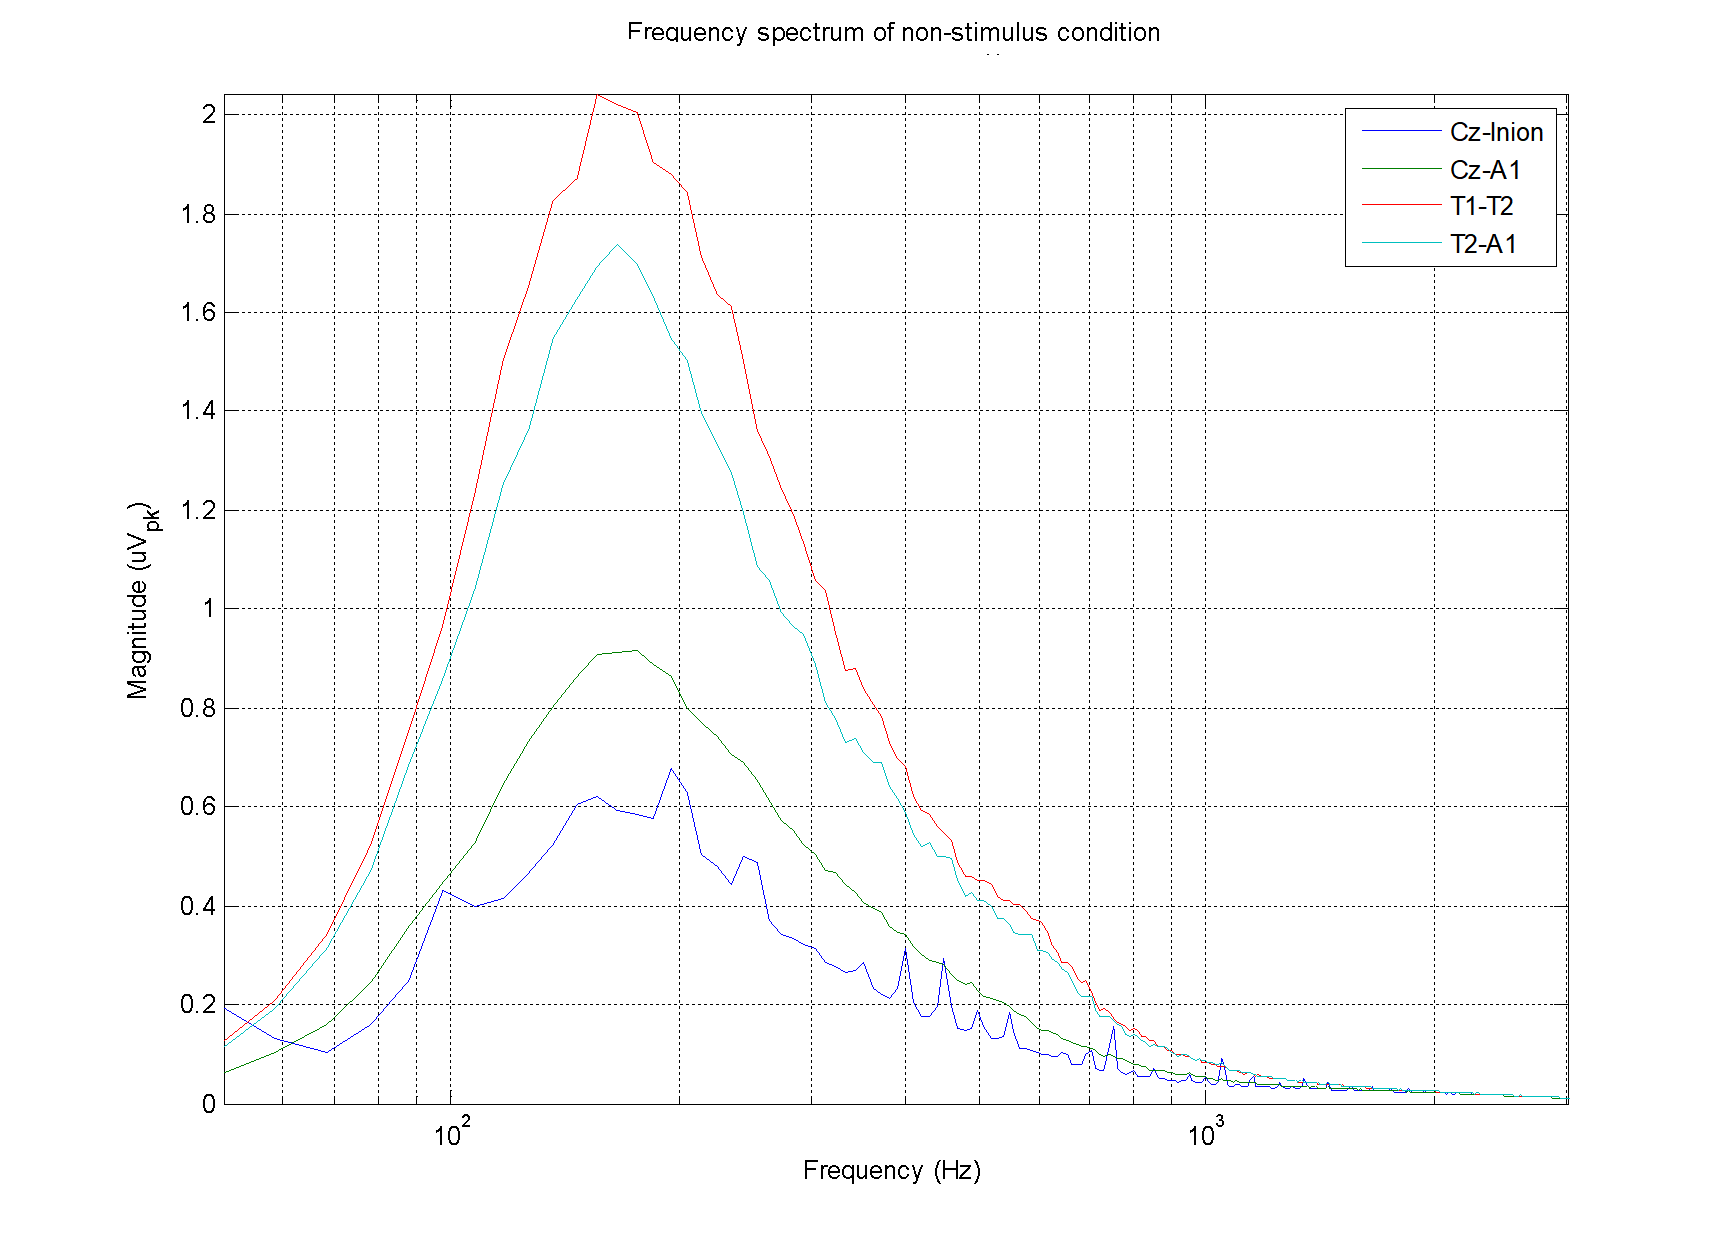
\includegraphics[width=0.5\textwidth]{images/FrequencyspectrumOfNon-StimulusCondition-1.png}
  \caption{噪声频谱}
  \label{fig:FrequencyspectrumOfNon-Stimulus}
\end{figure}
\subsubsection{通过波形平均改善信噪比}
作为基础处理步骤,所有ABR记录均经过以下预处理:
带通滤波(100-3000 Hz), 分段对齐(分析时窗15-25 ms),信号平均处理

下两图展示了定期计算的平均波形结果。随着叠加次数(Sweeps)的增加,ABR特征波的峰潜伏期界定愈加清晰。
\begin{figure}[H]
    \centering
    \begin{minipage}{0.48\textwidth}
        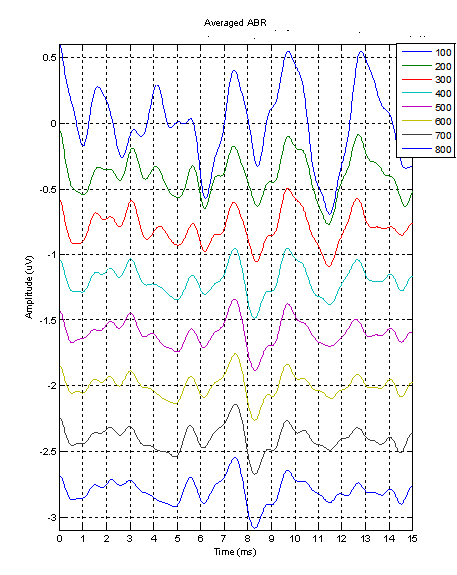
\includegraphics[width=\textwidth]{images/improvingSNRwaveformAveraging75.png}
    \end{minipage}
    \hfill
    \begin{minipage}{0.48\textwidth}
        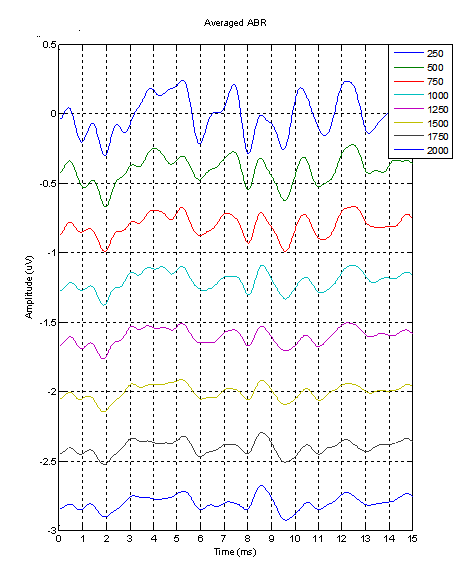
\includegraphics[width=\textwidth]{images/improvingSNRwaveformAveraging40.png}
    \end{minipage}
\end{figure}
在75 dB刺激强度下,受试者的短声刺激诱发波V潜伏期为7.2±0.3 ms,较已发表的标准值6.4±0.2 ms(使用插入式耳机时为5.6 ms+0.8 ms)偏高,可能与Neuroscan系统的触发同步时序问题有关。当改用500 HzTone刺激时,波V潜伏期延长至9.0±0.4 ms(相同强度)。

当刺激强度降至40 dB SL时,短声刺激的波V潜伏期为8.41±0.3 ms,而500 HzTone刺激则进一步延长至约10.8 ms。值得注意的是,低频Tone刺激在仅叠加2000次时,波V成分常难以通过视觉检测确认。

信号处理方法比较
通过 F$_{sp}$值评估了常规平均、加权平均和分块加权平均三种方法的性能如下图。由于受试者保持高度安静状态且记录期间背景噪声稳定,加权处理未显现优势。有趣的是,虽然Cz-Inion导联记录的波V-V'振幅较大,但其背景噪声水平显著高于Cz-A1导联,导致 F$_{sp}$比值明显降低。


\begin{figure}[H]
    \centering
    \begin{minipage}{0.48\textwidth}
        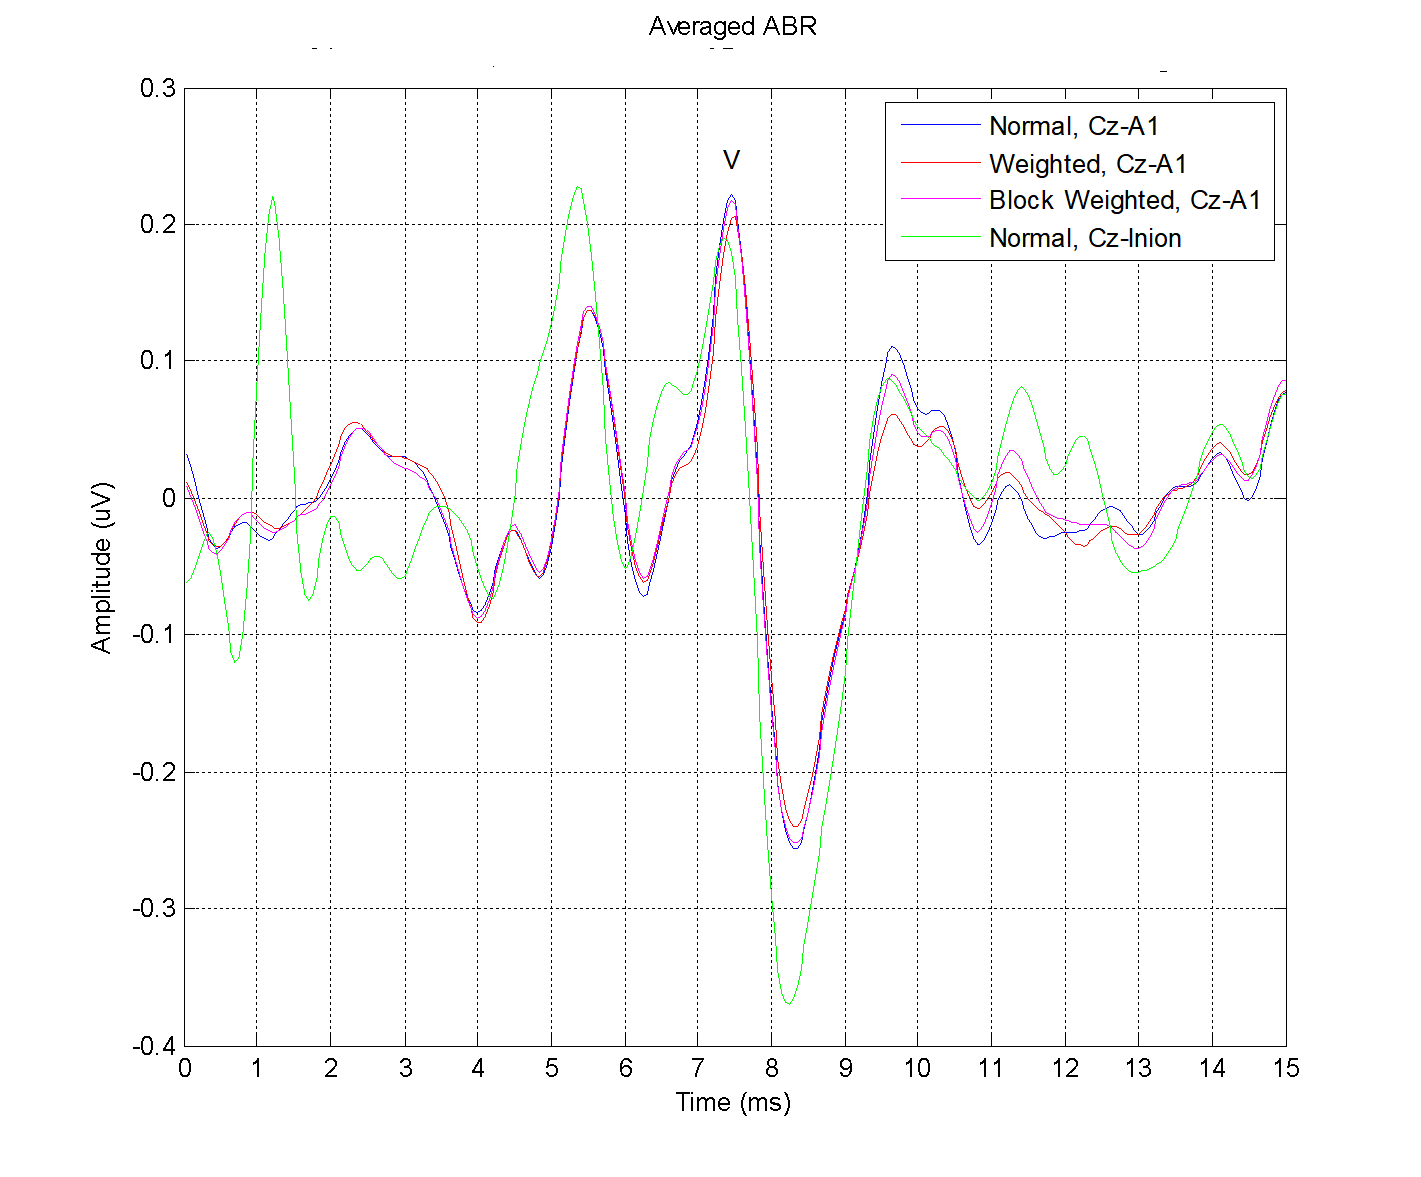
\includegraphics[width=\textwidth]{images/click75dbABR.png}
    \end{minipage}
    \hfill
    \begin{minipage}{0.48\textwidth}
        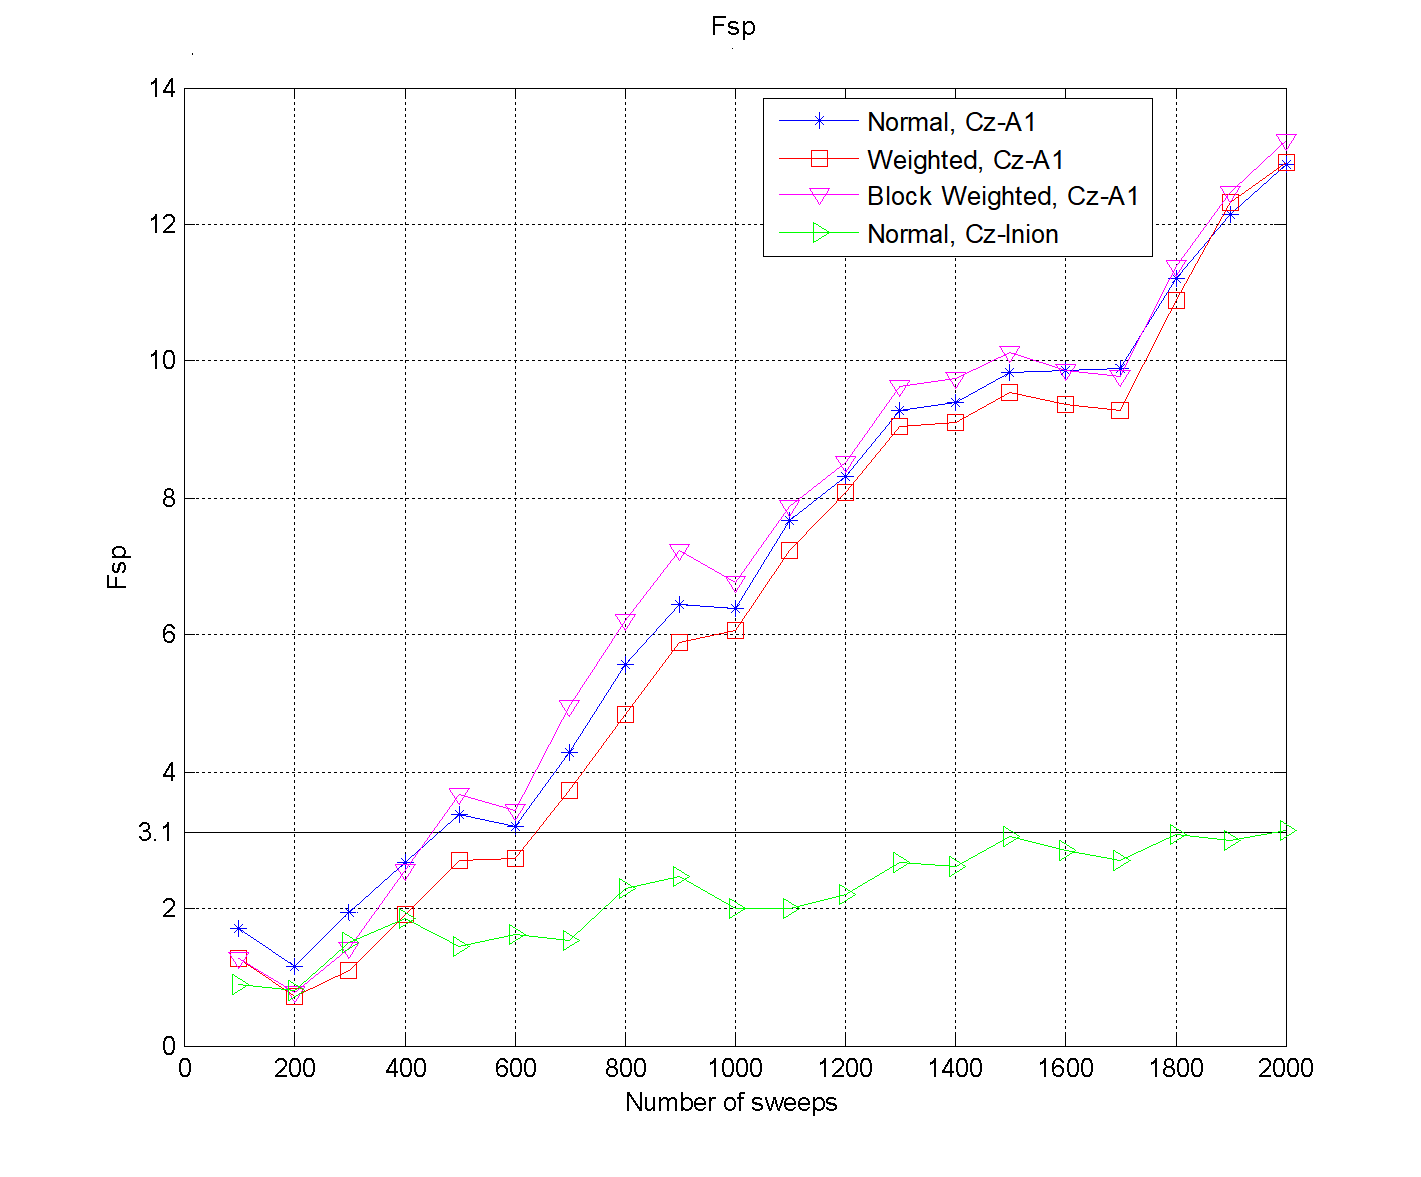
\includegraphics[width=\textwidth]{images/click75dbABRfsp.png}
    \end{minipage}
    
    \vspace{0.2cm}
    
    \begin{minipage}{0.48\textwidth}
        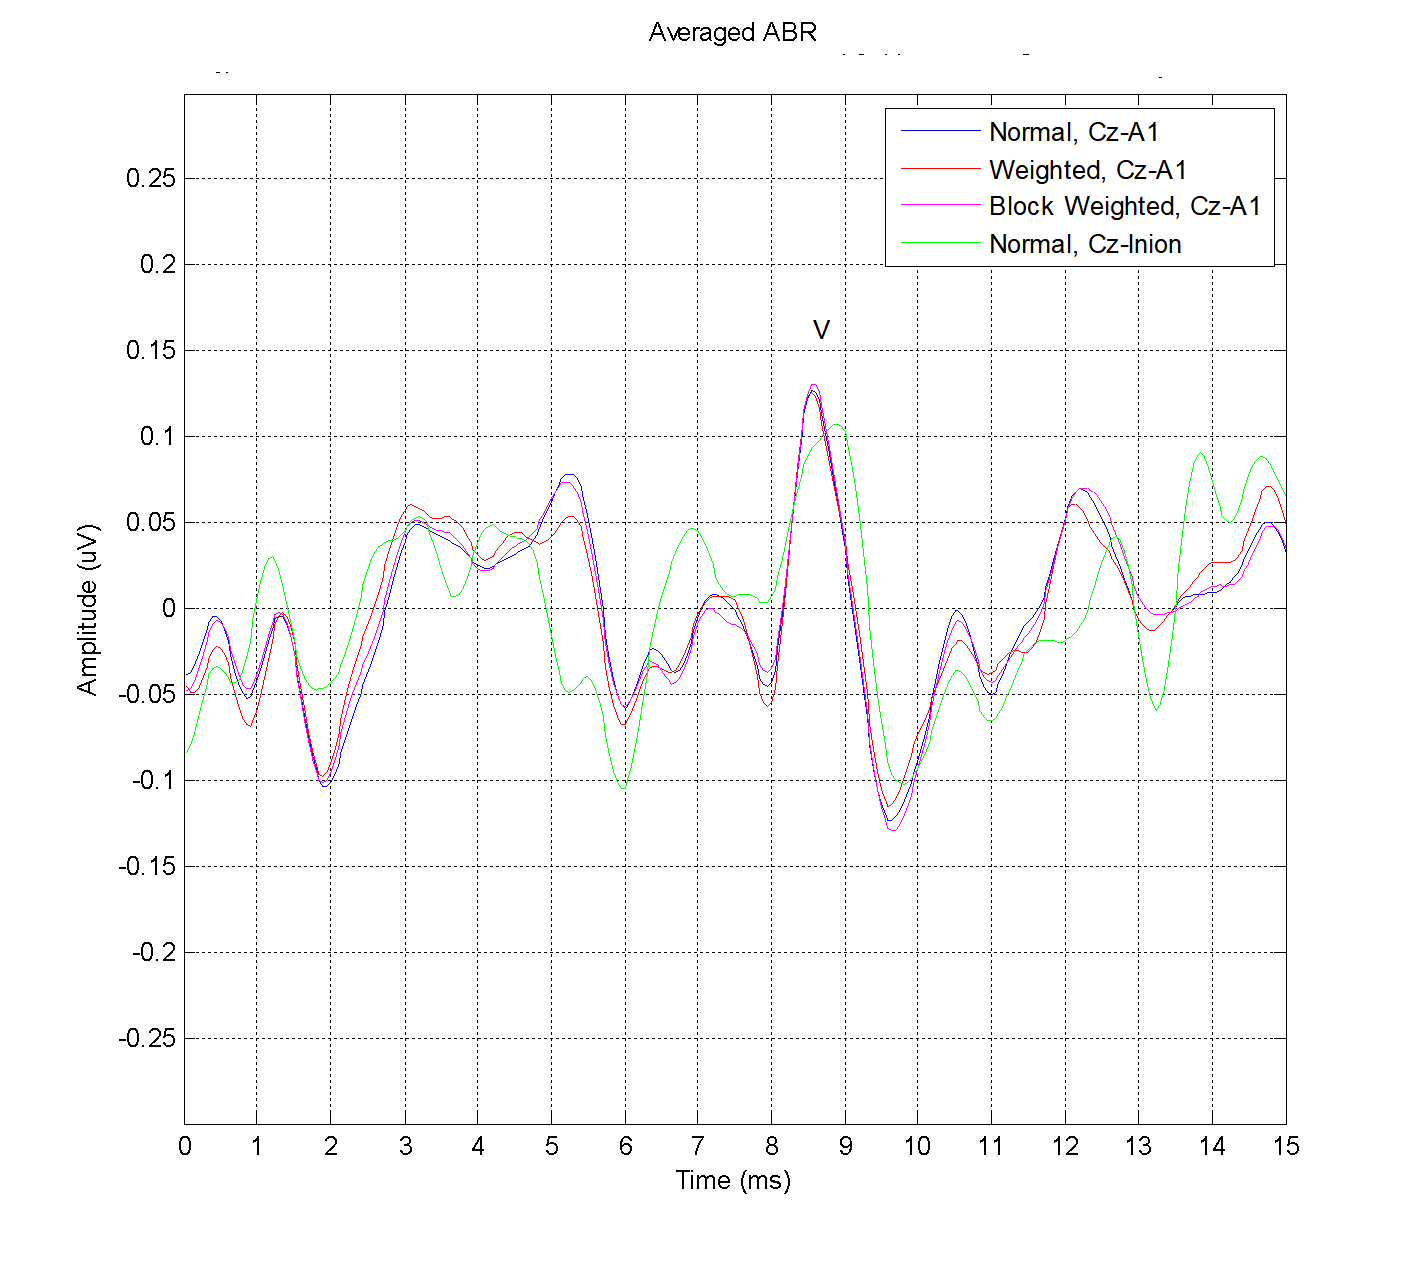
\includegraphics[width=\textwidth]{images/click40dbABR.png}
    \end{minipage}
    \hfill
    \begin{minipage}{0.48\textwidth}
        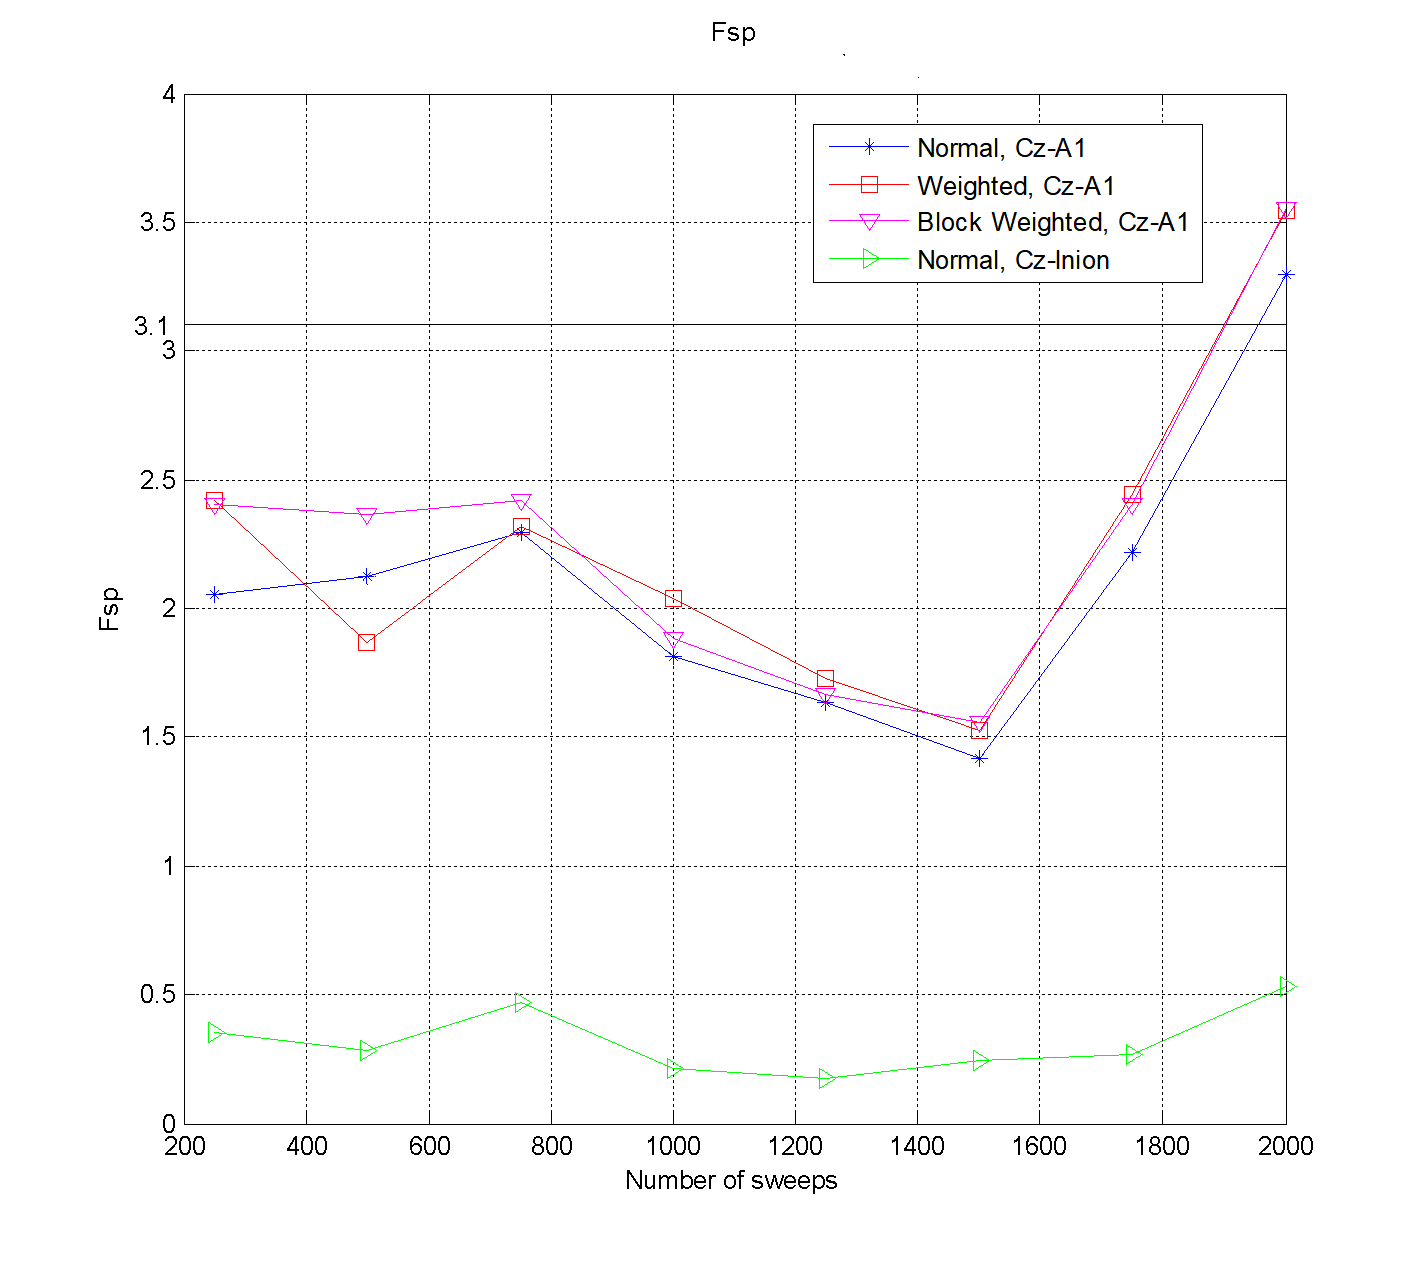
\includegraphics[width=\textwidth]{images/click40dbABRfsp.png}
    \end{minipage}
    \caption{常规平均、加权平均和分块加权平均在75,40 dB的潜伏期和性能}
    \label{fig:7540ABRAndFsp}
\end{figure}

\subsubsection{Chirp刺激诱发的响应}
\paragraph{宽带Chirp}
在40 dB SL刺激强度下,受试者的波V-V'峰峰值振幅显著增强,而在75 dB SL下振幅反而降低。

Chirp刺激在低刺激强度(20–40 dB SL)下的增强效应与Dau等(2000)\cite{dau2000optimized}的研究一致,该研究发现波V振幅在低强度下显著增大,但在50–60 dB SL时无此优势。这可能是因为高强度刺激下,低频能量同时刺激耳蜗基底区,导致神经反应同步性降低,部分抵消了重叠响应峰的增强效果。
\begin{table}[H]
\centering
\caption{不同刺激条件下波V-V'振幅及Chirp刺激改善率}
\label{tab:wave_amplitude}
\begin{tabular}{llcc}
\toprule
\multicolumn{1}{c}{\textbf{刺激强度}} & \multicolumn{1}{c}{\textbf{刺激类型}} & \textbf{波V-V'振幅 (uV)} & \textbf{改善率} \\
\midrule
\multirow{6}{*}{75 dB SL} & \multicolumn{3}{l}{\textbf{受试者 LC}} \\
 & Click (负极性) & 0.36 & \\
 & Click (正极性) & 0.45 & \\
 & Chirp & 0.27 & -(27-41)\% \\
\cmidrule{2-4}
 & \multicolumn{3}{l}{\textbf{受试者 DR}} \\
 & Click (负极性) & 0.46 & \\
 & Click (正极性) & 0.47 & \\
 & Chirp & 0.25 & -46 \\
\midrule
\multirow{6}{*}{40 dB SL} & \multicolumn{3}{l}{\textbf{受试者 LC}} \\
 & Click (负极性) & 0.22 & \\
 & Click (正极性) & 0.17 & \\
 & Chirp & 0.46 & +(100-156)\% \\
\cmidrule{2-4}
 & \multicolumn{3}{l}{\textbf{受试者 DR}} \\
 & Click (负极性) & 0.23 & \\
 & Click (正极性) & 0.13 & \\
 & Chirp & 0.32 & +(33-146)\% \\
\bottomrule
\end{tabular}
\smallskip
\footnotesize
\textsuperscript{*} 改善率计算基于与同条件下最优Click刺激值的比较,范围值表示不同极性刺激的对比结果
\end{table}
\newpage
\paragraph{特定频率Chirp}
针对4000 Hz和500 Hz频率的刺激,比较了窄带Chirp刺激引起的反应与Tone刺激引起的反应。
\begin{figure}[H]
    \centering
    \begin{minipage}{0.48\textwidth}
        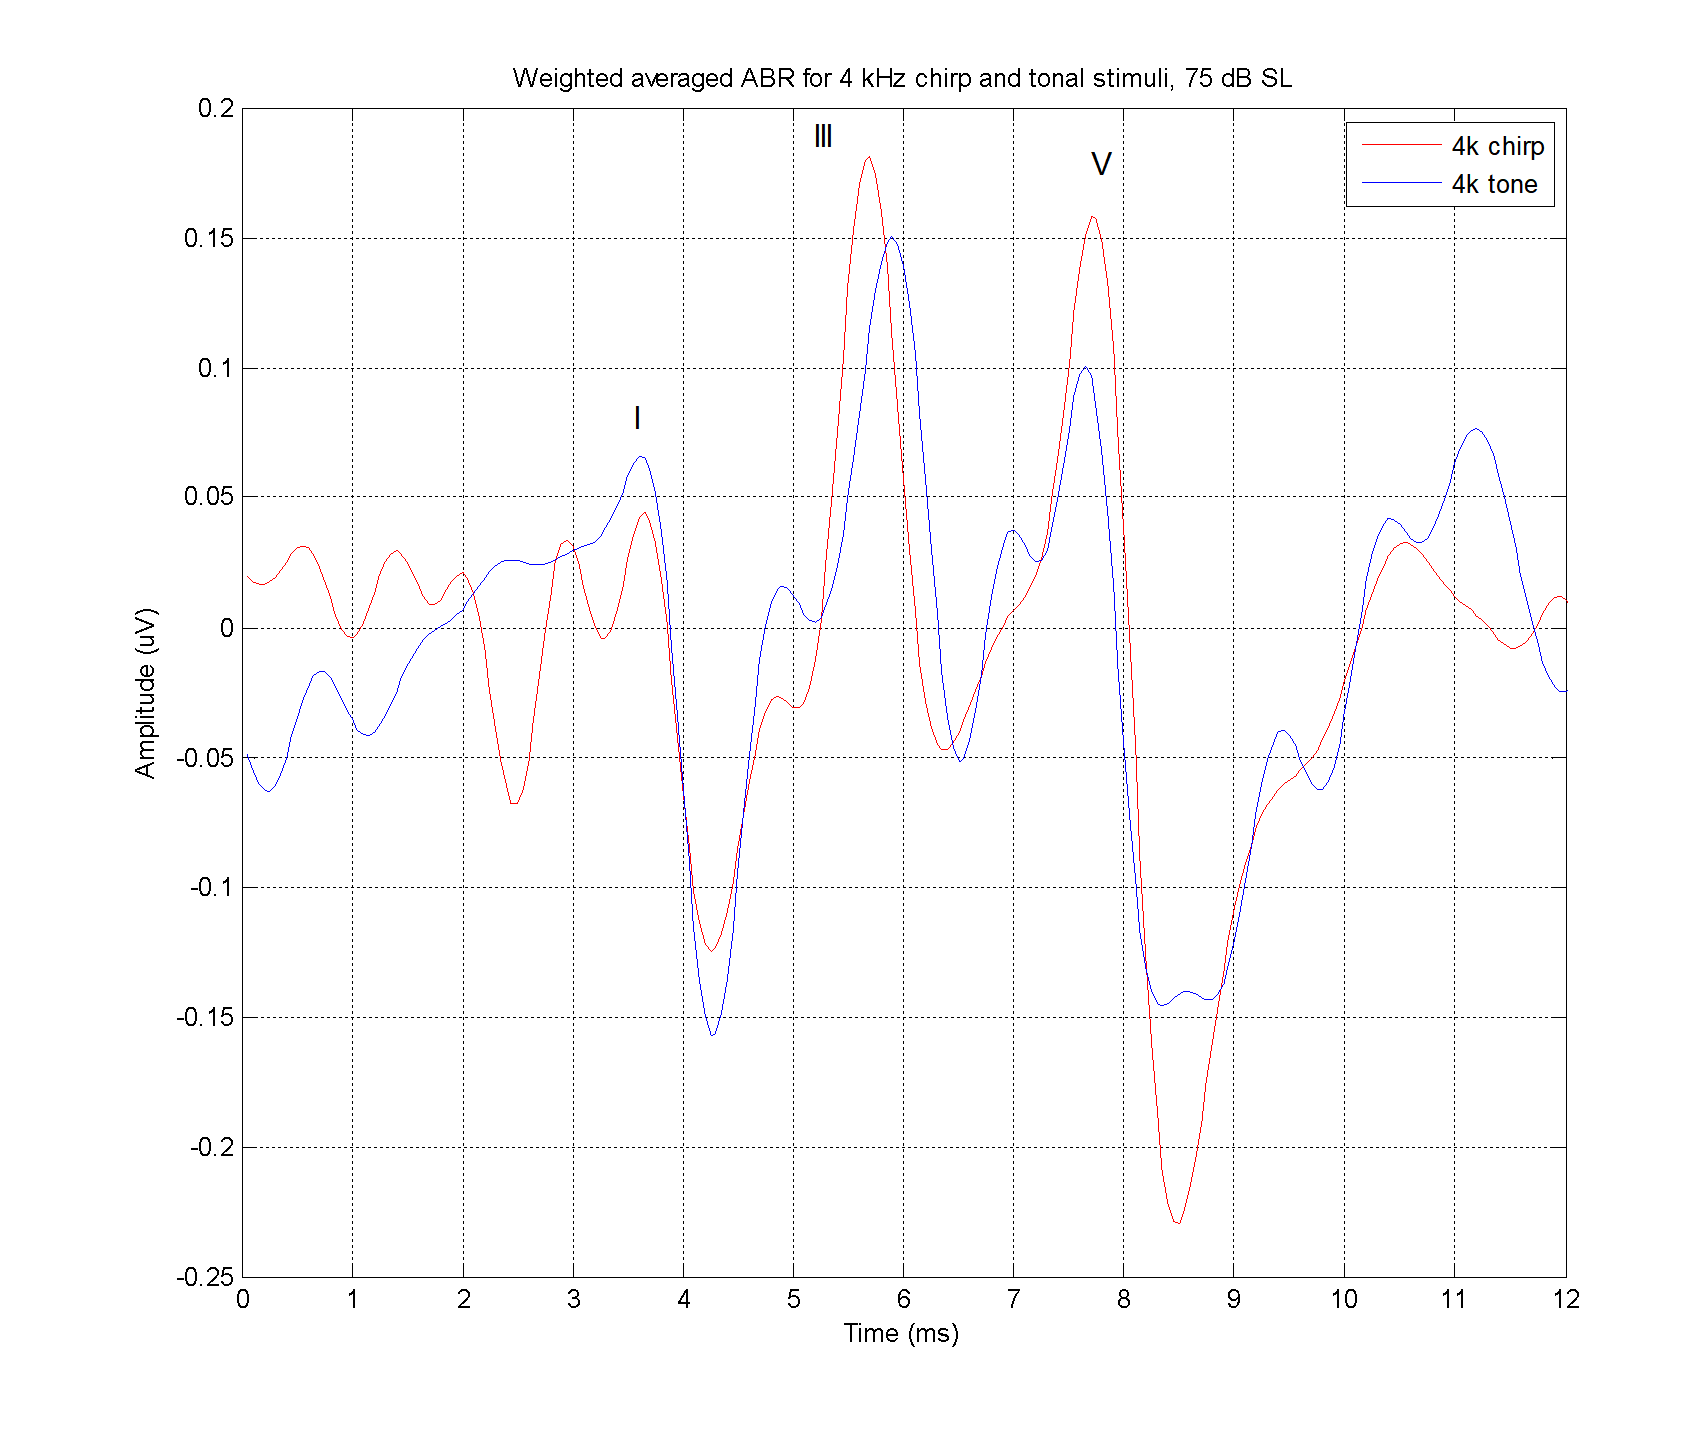
\includegraphics[width=\textwidth]{images/4kchirpAndTonalStimuli75db.png}
    \end{minipage}
    \hfill
    \begin{minipage}{0.48\textwidth}
        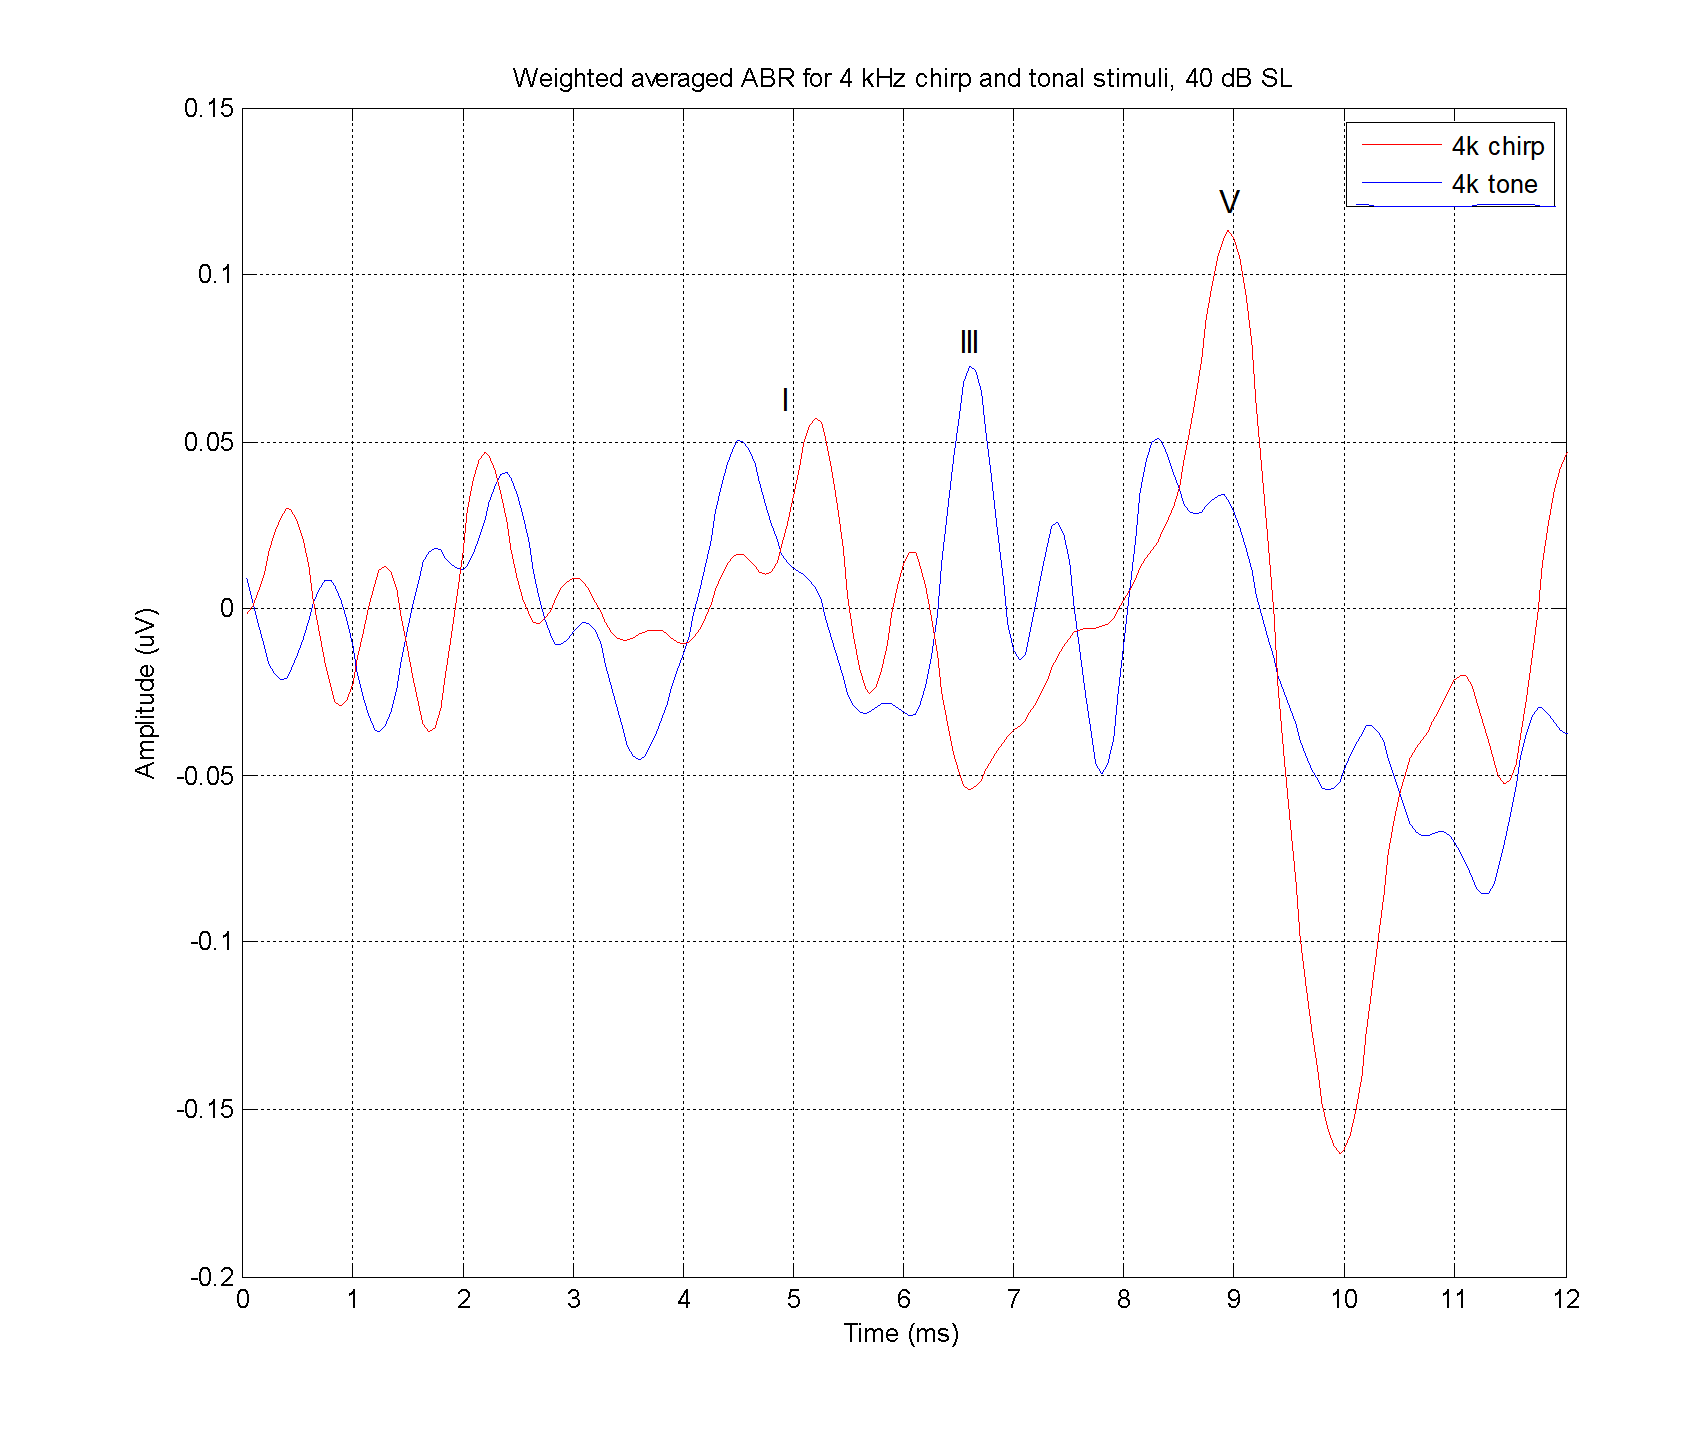
\includegraphics[width=\textwidth]{images/4kchirpAndTonalStimuli40db.png}
    \end{minipage}
    
    \vspace{0.2cm}
    
    \begin{minipage}{0.48\textwidth}
        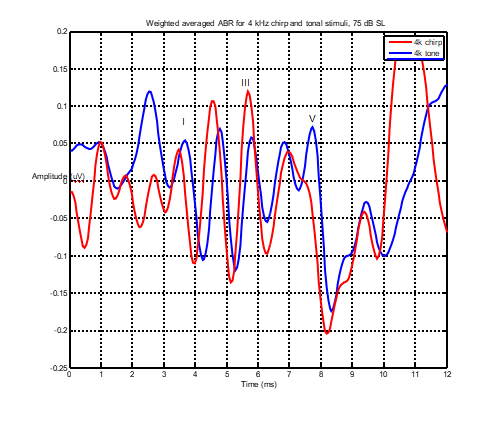
\includegraphics[width=\textwidth]{images/4kchirpAndTonalStimuli75db2.png}
    \end{minipage}
    \hfill
    \begin{minipage}{0.48\textwidth}
        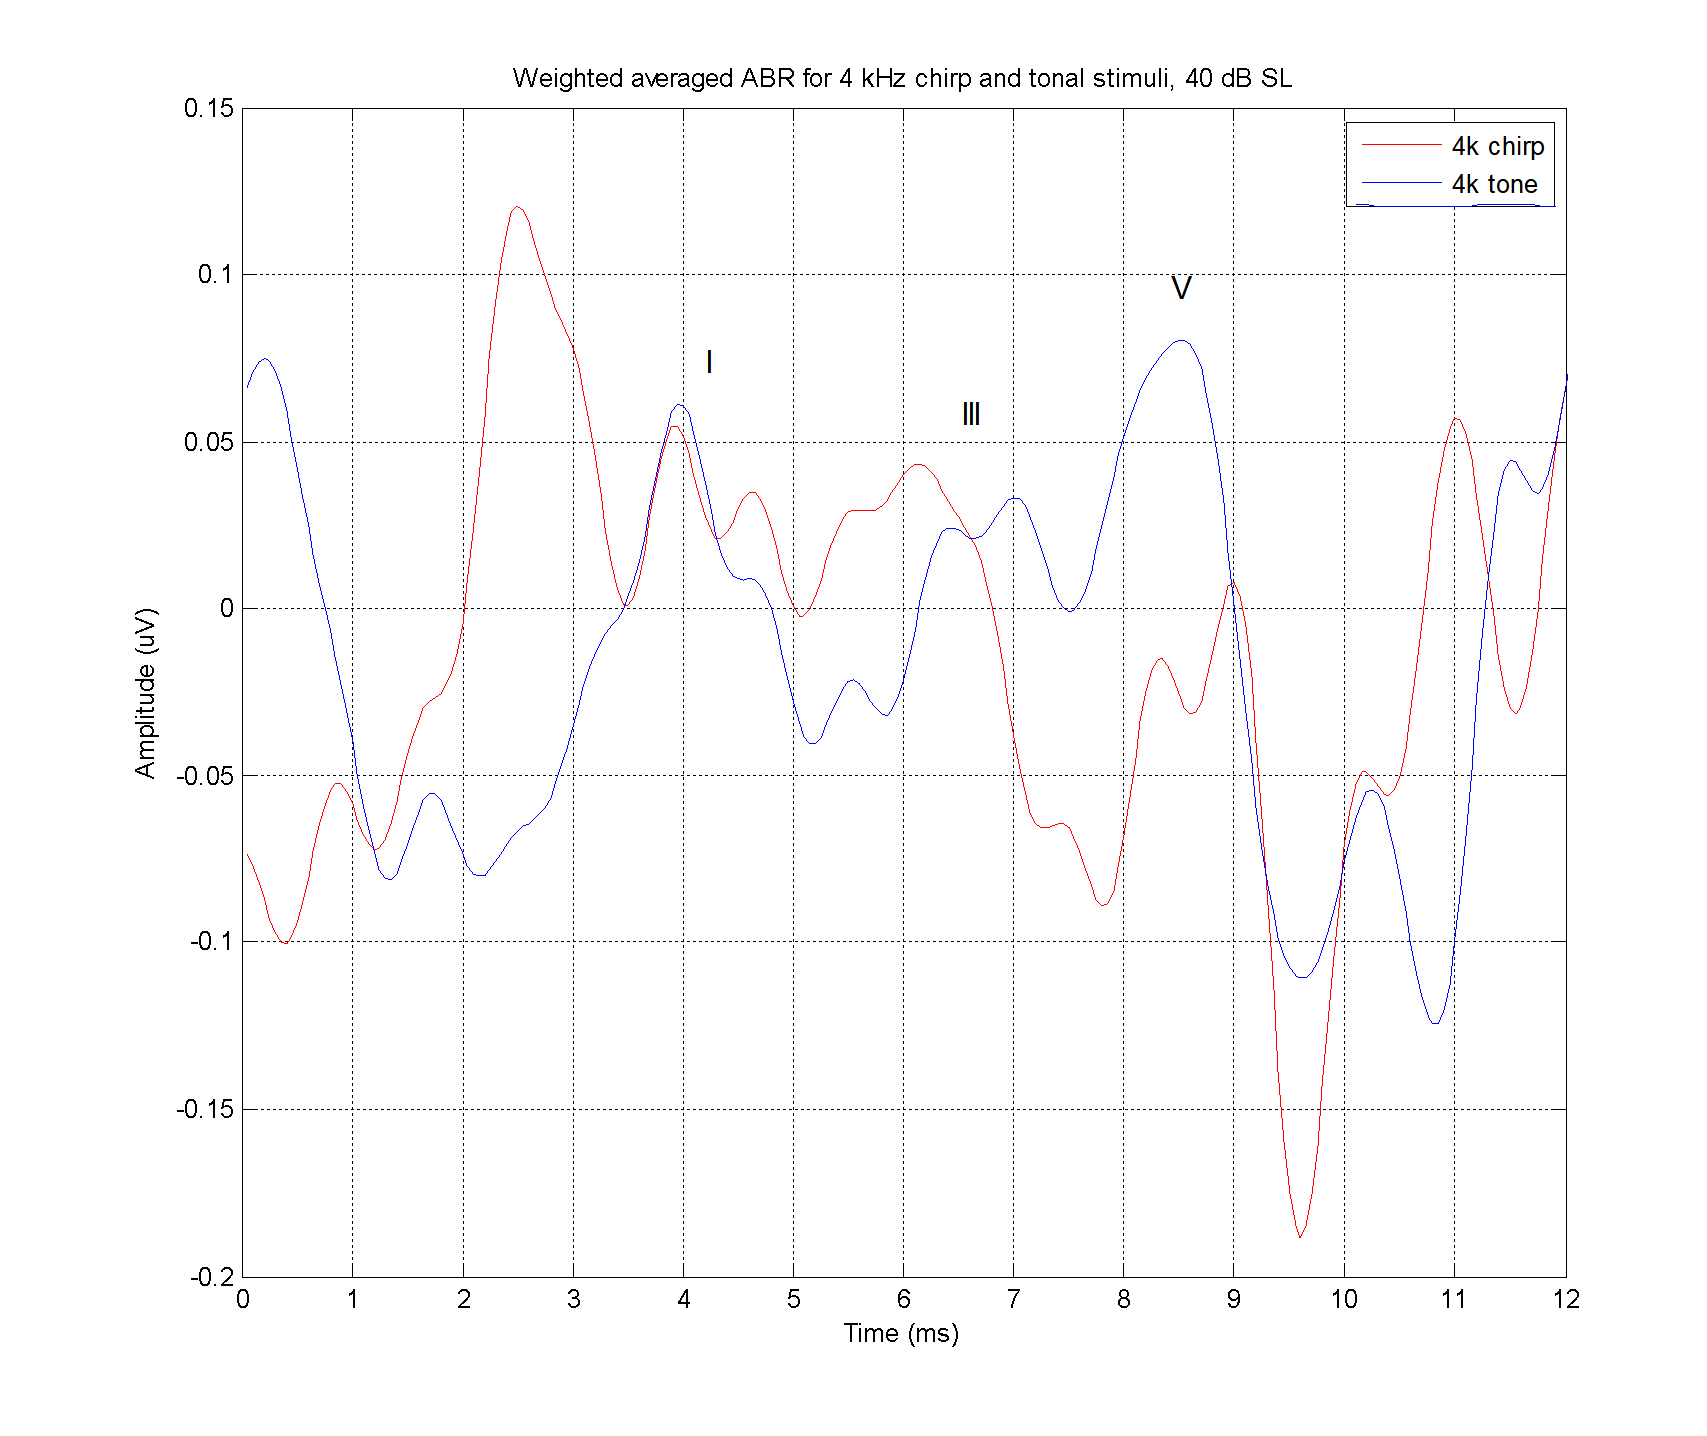
\includegraphics[width=\textwidth]{images/4kchirpAndTonalStimuli40db2.png}
    \end{minipage}
    \caption{两个测试者的4 kHz 窄带Chirp声和Tone刺激}
    \label{fig:twotester4kchirpandtone}
\end{figure}
对于受试者1,在75 dB SL强度下,Chirp声刺激诱发的V波振幅为156 nV,Tone刺激为100 nV,增幅达56\%。在40 dB SL强度下,效果更为显著:Chirp声刺激的V波振幅为110 nV,Tone刺激仅50 nV(增幅120\%)。
对于受试者2,无论是75 dB SL还是40 dB SL强度,Chirp声与Tone刺激的V波峰峰值(V-V’)振幅均基本一致。

与4 kHz刺激响应相比500 HzTone刺激经过2000次叠加后的平均响应表现出显著更高的噪声水平。无论是75 dB SL还是40 dB SL强度,Chirp刺激诱发的波V振幅与Tone刺激相比均呈现相似或降低的趋势。值得注意的是,受试者1在40 dB SL强度下的响应未出现预期的峰值/潜伏期特征(可能源于记录误差或过量噪声),该数据已在后续分析中剔除。

\textbf{主要发现:}
Chirp刺激对波V振幅的提升效果在不同受试者及刺激频率间缺乏一致性。然而总体而言,研究证实Chirp刺激在以下方面具有优势:

宽带频率响应检测

4 kHz高频信号采集

低刺激强度(≤40 dB SL)条件下的信号增强

\subsubsection{交错频率刺激的响应特征}
本研究采用含噪声掩蔽(GHINOMA)和无掩蔽条件的交错频率Tone/Chirp刺激序列(4000、2000、1000、500 Hz)采集数据。
\paragraph*{无噪声掩蔽刺激序列参数}

实验采用精确定时的多频刺激序列设计:\textbf{时序参数}设置包含高频至低频的切换间隔(18 ms)和序列循环间隔(50 ms,位于500 Hz刺激后),据此计算得总周期时长$T_{\text{total}} = 3 \times 18,\text{ms} + 50,\text{ms} = 104,\text{ms}$。\textbf{刺激效率}通过有效速率公式$R_{\text{eff}} = \frac{1000}{104,\text{ms}/4} \approx 38.5,\text{Hz}$确定,在5秒记录时长内可完成$5,\text{s} \times 38.5,\text{Hz} = 192$次扫描。该设计通过$\frac{104,\text{ms}}{\text{周期}}$的紧凑时序实现了频段间的快速切换与信号的高效采集。
\begin{figure}[H]
    \centering
    \begin{minipage}{0.48\textwidth}
        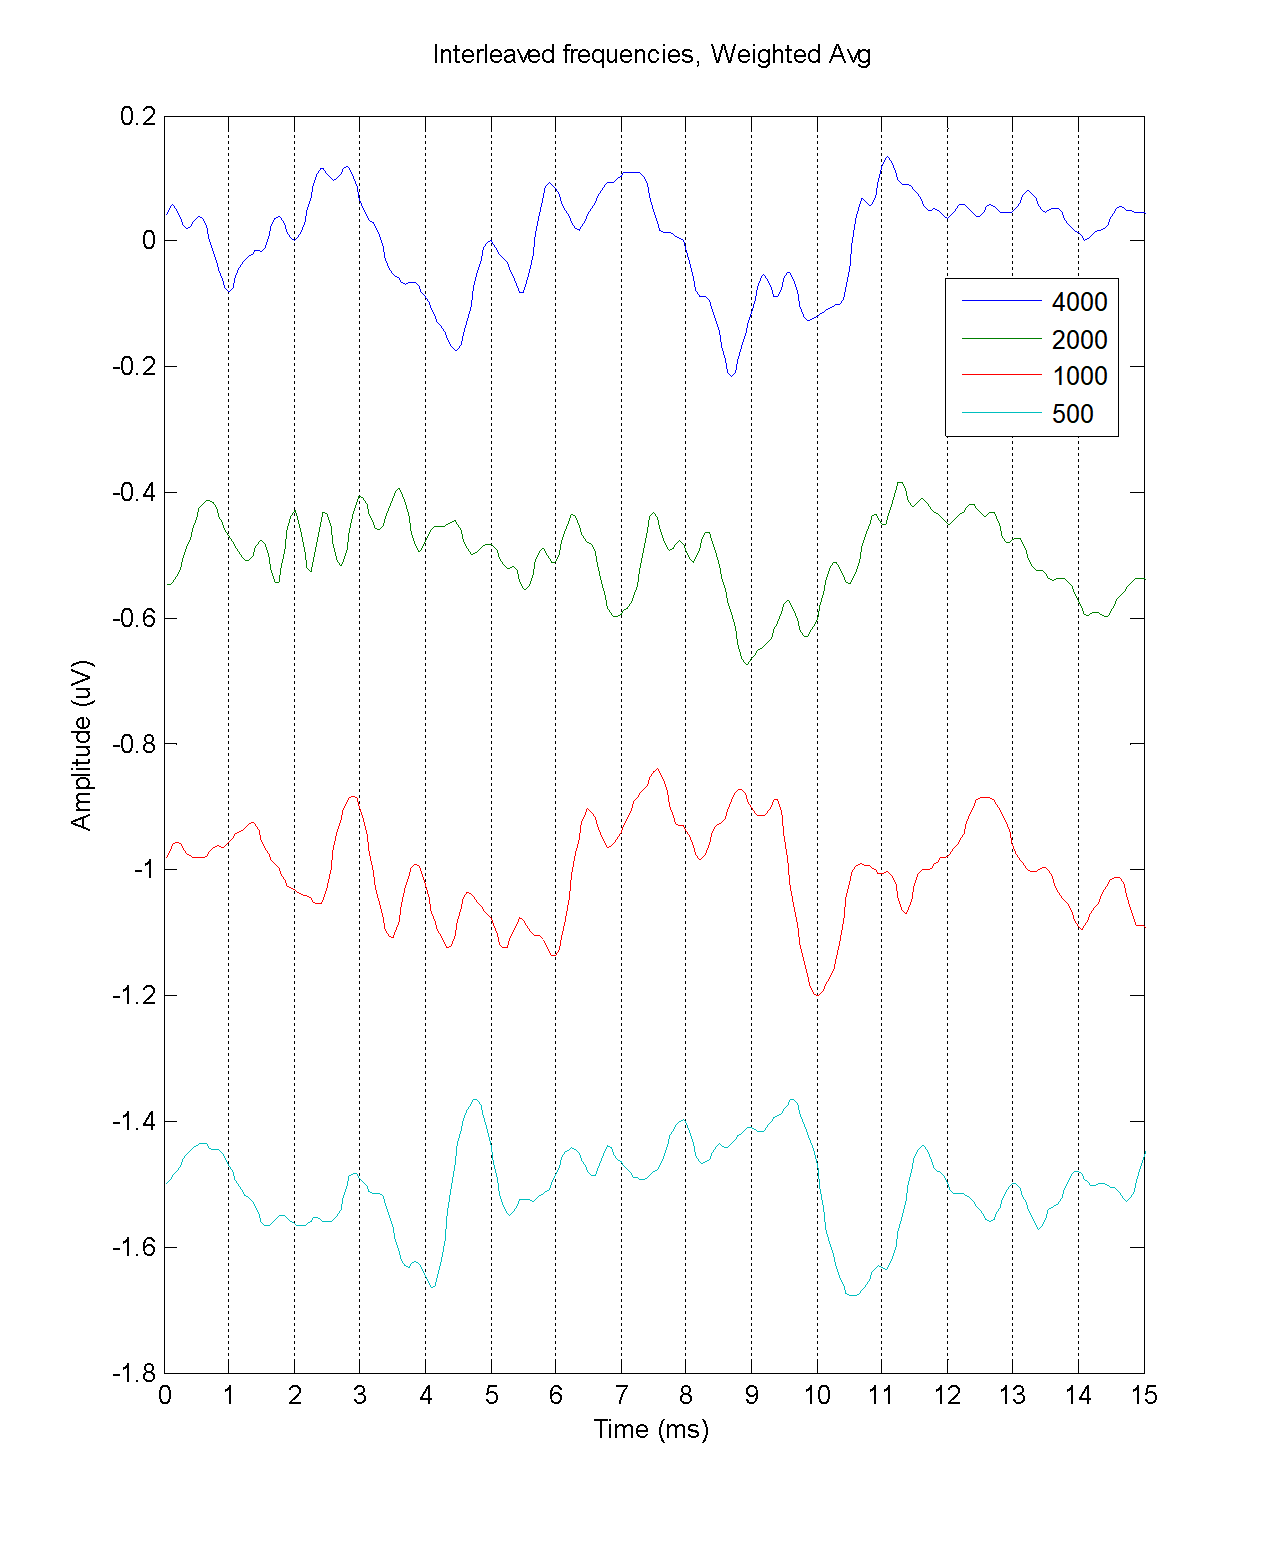
\includegraphics[width=\textwidth]{images/Interleaved75dbGHINOMA-1.png}
    \end{minipage}
    \hfill
    \begin{minipage}{0.48\textwidth}
        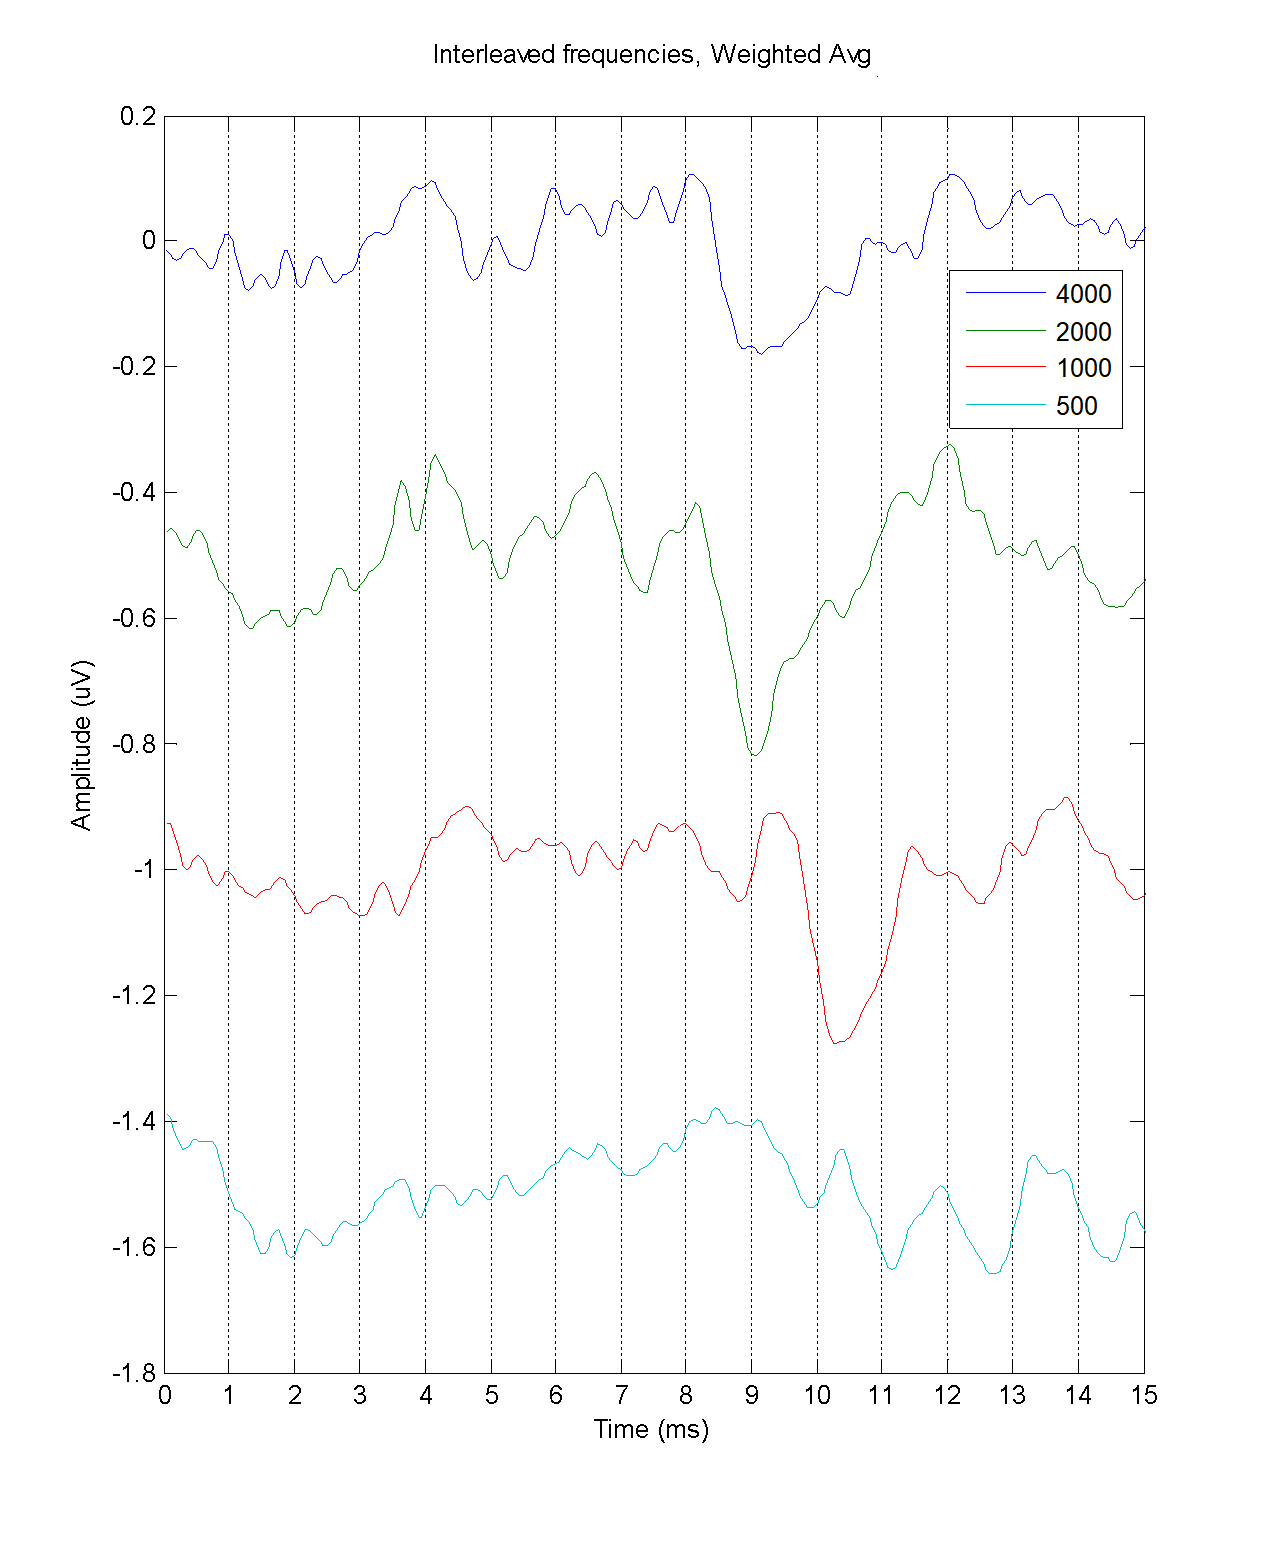
\includegraphics[width=\textwidth]{images/Interleaved75dbGHINOMA-2.png}
    \end{minipage}
    
    \vspace{0.2cm}
    
    \begin{minipage}{0.48\textwidth}
        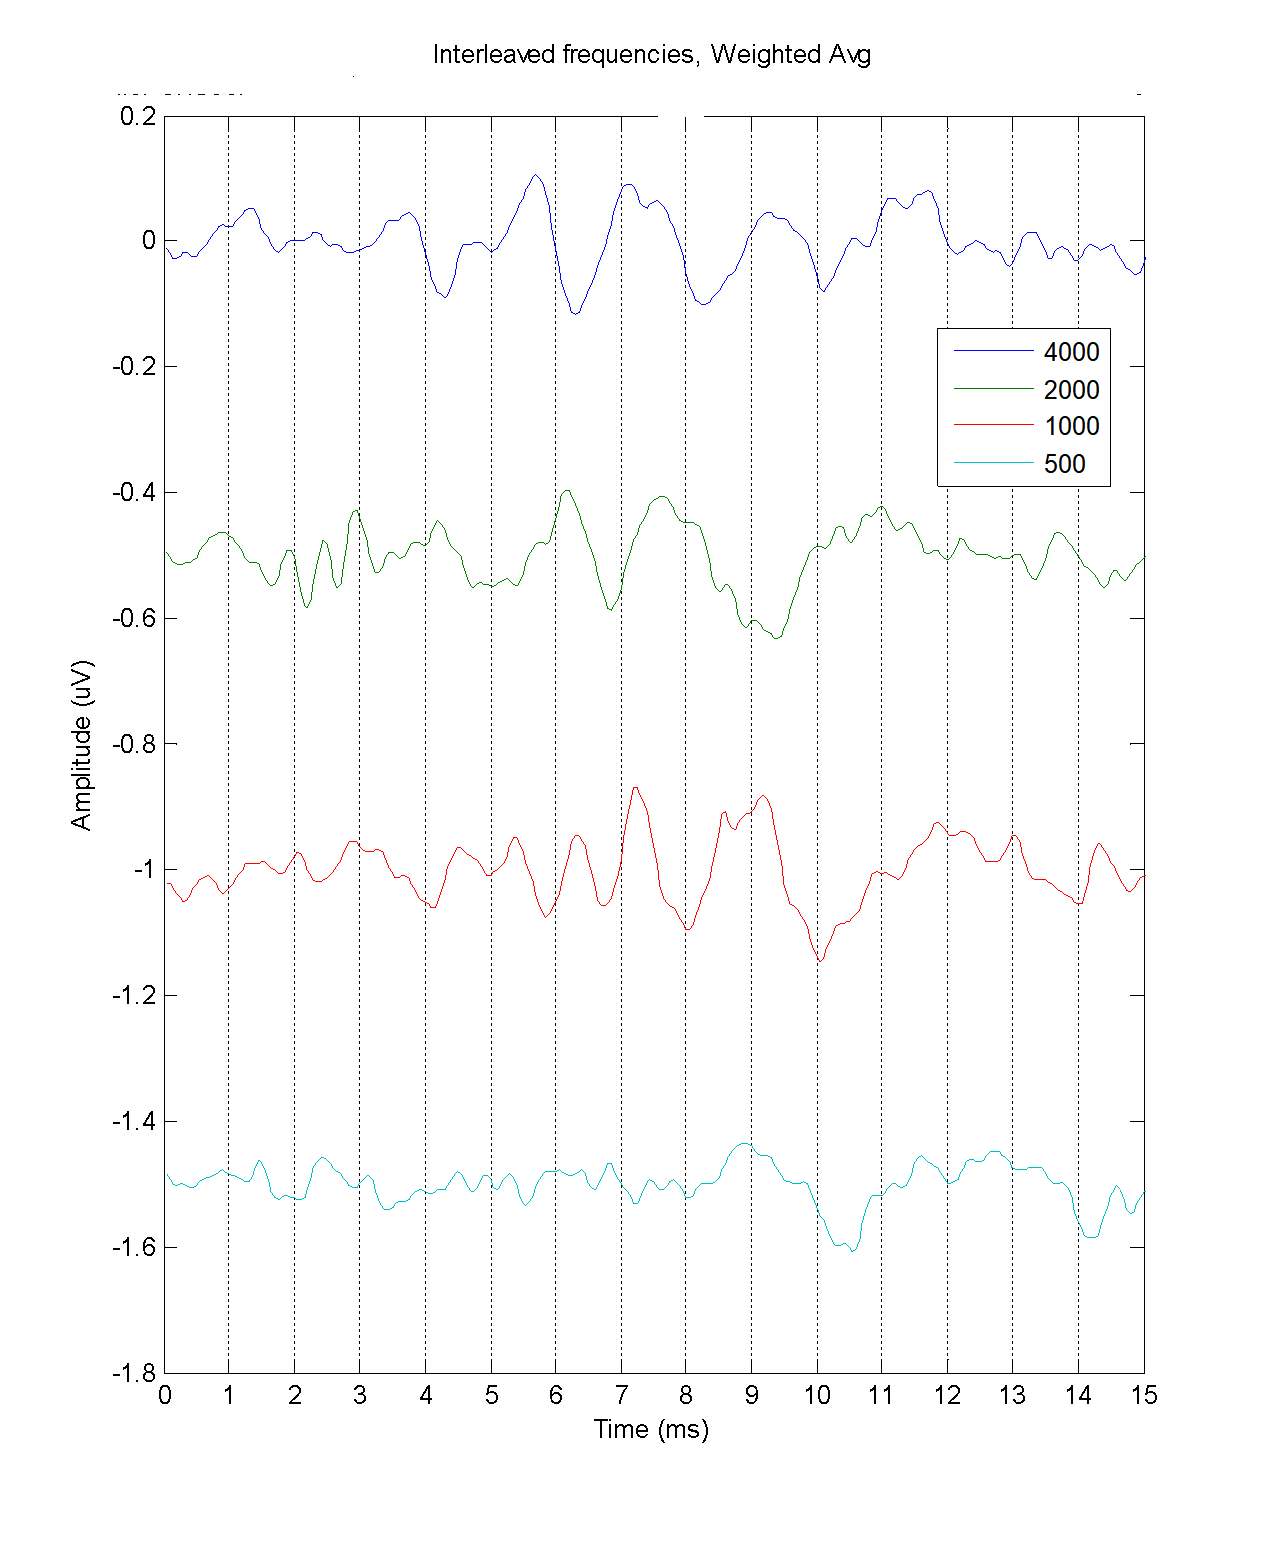
\includegraphics[width=\textwidth]{images/Interleaved75dbGHINOMA-3.png}
    \end{minipage}
    \hfill
    \begin{minipage}{0.48\textwidth}
        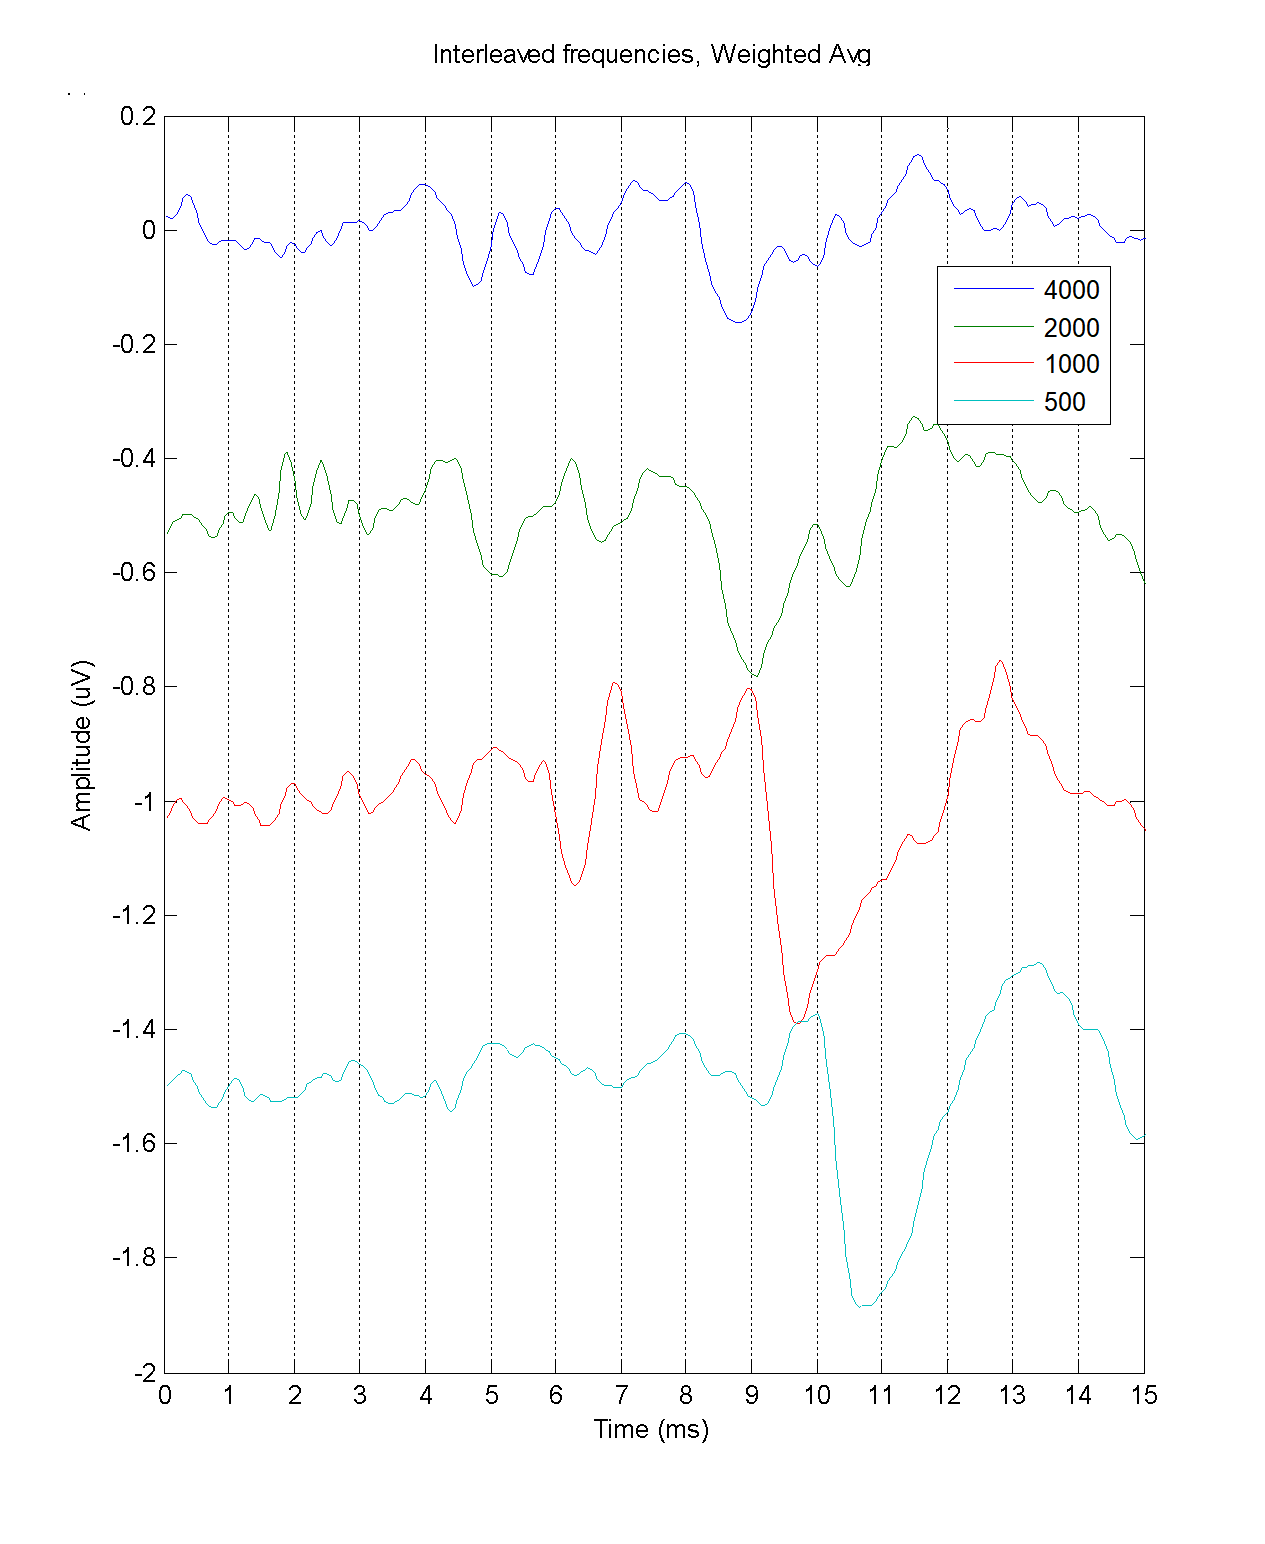
\includegraphics[width=\textwidth]{images/Interleaved75dbGHINOMA-4.png}
    \end{minipage}
    \caption{交替Tone(4kHz、2kHz、1kHz、500Hz)ABR 波形}
    \label{fig:Interleaved75dbGHINOMA}
\end{figure}


\begin{figure}[H]
    \centering
    \begin{minipage}{0.48\textwidth}
        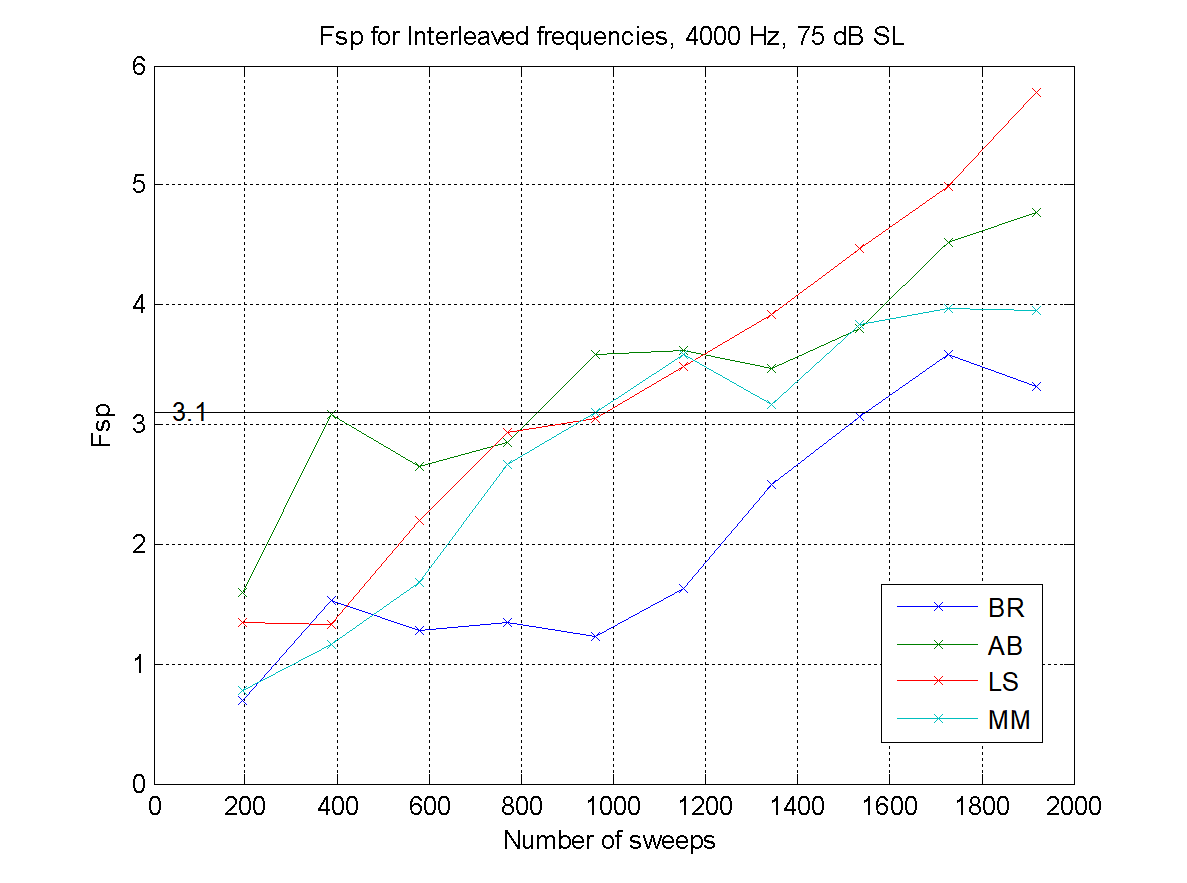
\includegraphics[width=\textwidth]{images/fspForInterleaved4000.png}
    \end{minipage}
    \hfill
    \begin{minipage}{0.48\textwidth}
        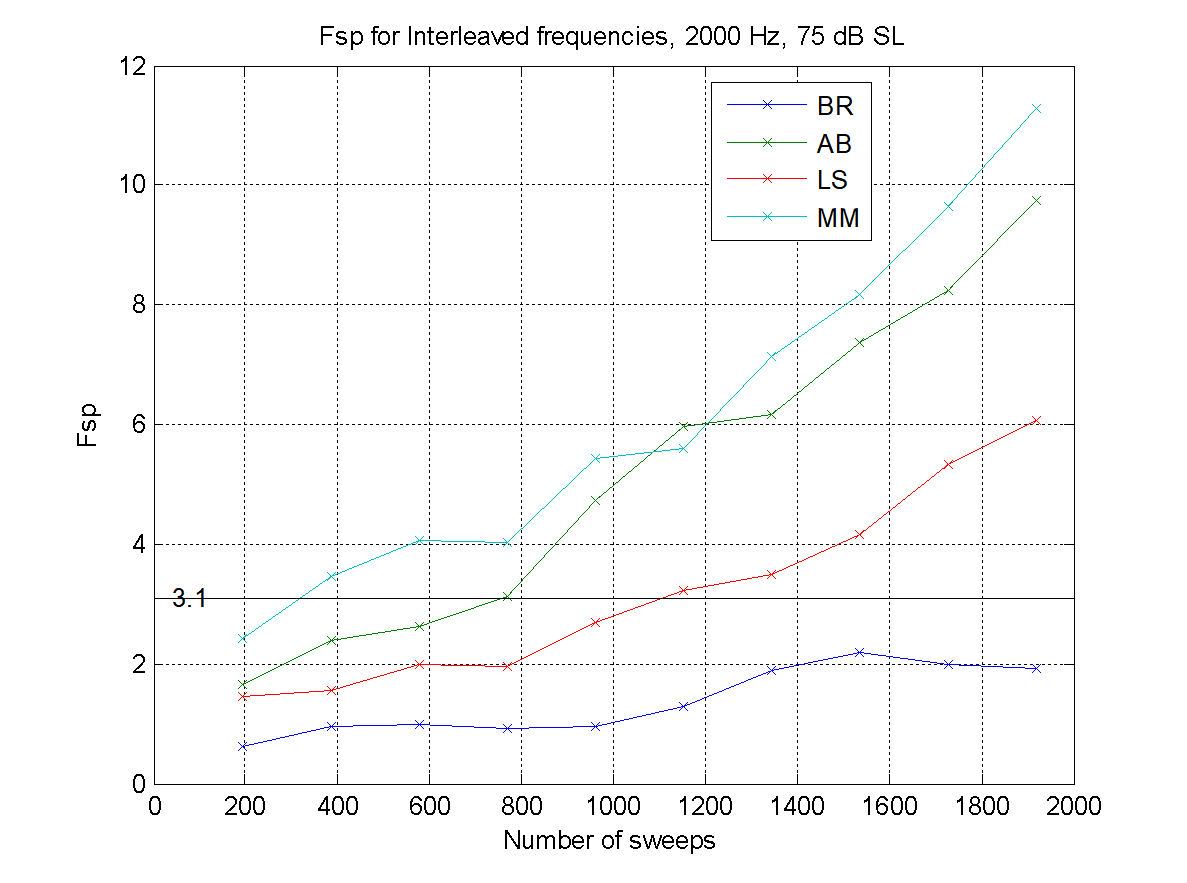
\includegraphics[width=\textwidth]{images/fspForInterleaved2000.png}
    \end{minipage}
    
    \vspace{0.2cm}
    
    \begin{minipage}{0.48\textwidth}
        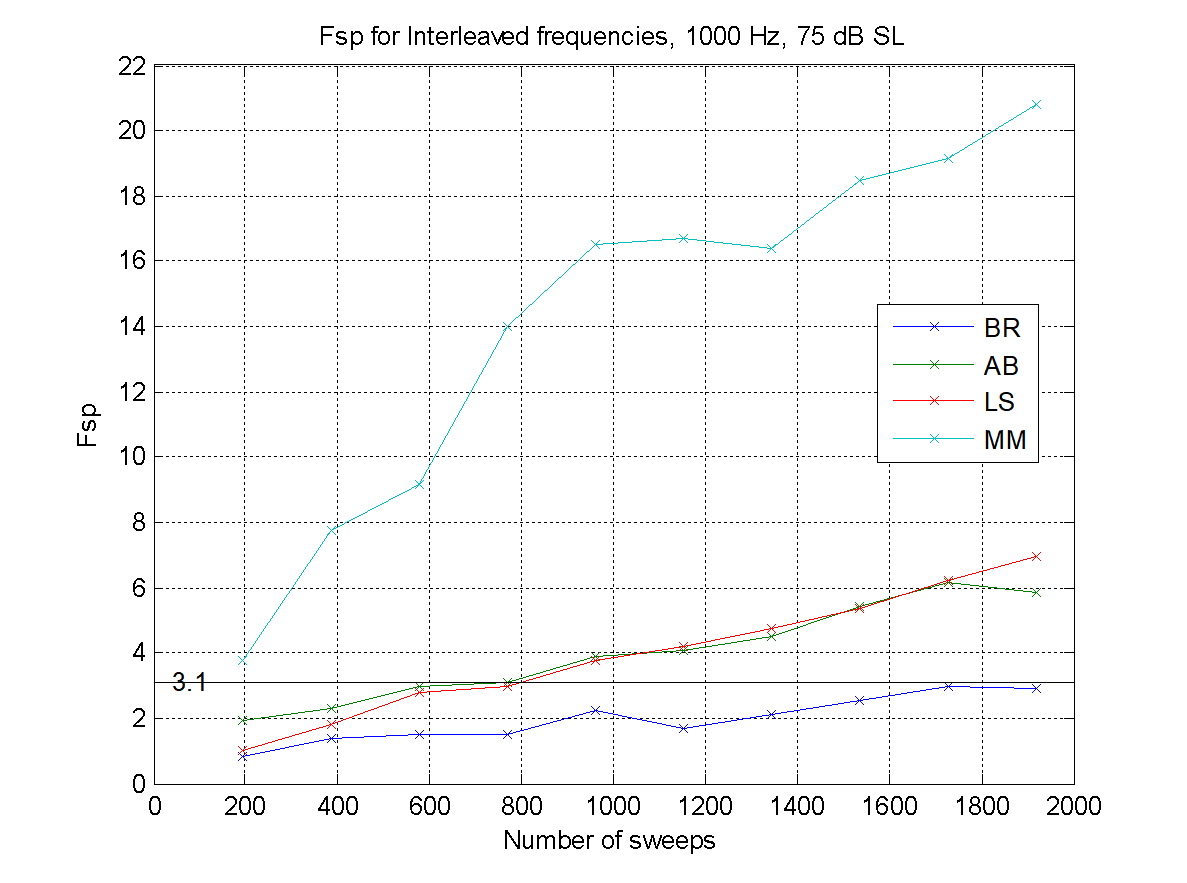
\includegraphics[width=\textwidth]{images/fspForInterleaved1000.png}
    \end{minipage}
    \hfill
    \begin{minipage}{0.48\textwidth}
        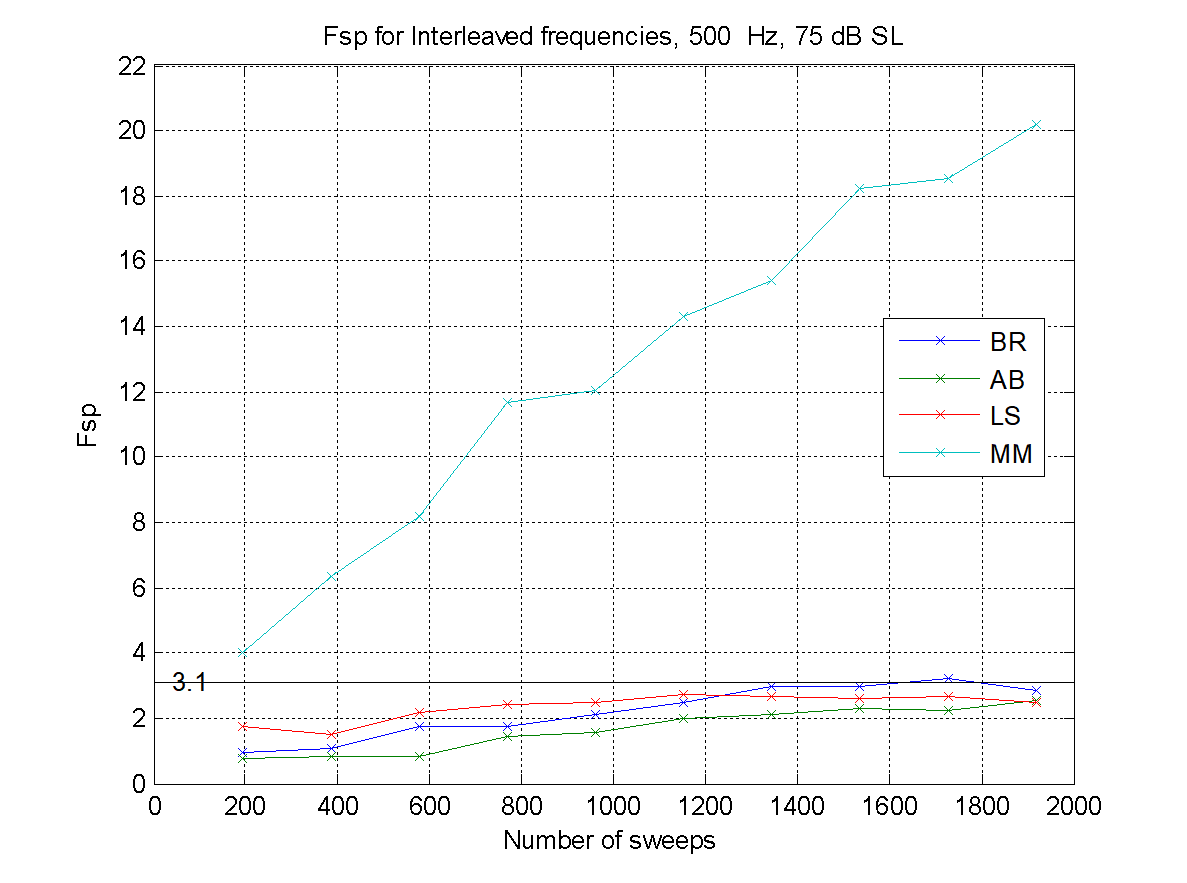
\includegraphics[width=\textwidth]{images/fspForInterleaved500.png}
    \end{minipage}
    \caption{交替Tone(4kHz、2kHz、1kHz、500Hz) F$_{sp}$ }
    \label{fig:Interleaved75dbGHINOMA}
\end{figure}

\paragraph*{带高通噪声掩蔽的交错频率刺激}
采用GHINOMA高通噪声掩蔽的交错频率刺激序列中的Tone刺激,与20 Hz呈现速率的单频刺激存在以下关键差异:
所有频率的Tone短声持续时间统一约为3 ms;采用高斯窗(Gaussian window)进行时域加窗处理
;
无噪声掩蔽条件下的刺激序列统一采用65 dB。

在交错频率刺激序列中,Chirp刺激与Tone刺激的F{$_sp$}比值存在显著频率依赖性差异:

\begin{itemize}
\item \textbf{4000 Hz与1000 Hz}:Chirp刺激的F$_{sp}$比值显著更高($p<0.05$)
\item \textbf{其他测试频率}:未观察到统计学显著差异
\end{itemize}

\textbf{主要结论:}
在本研究有限样本量条件下:

\begin{itemize}
\item 可识别响应所需的平均测试时长未显著缩短
\item 波形形态学特征的可解释性降低
\end{itemize}

\subsubsection{基于MLS的ABR响应}
MLS采用高刺激率的伪随机序列,通过快速连续呈现刺激信号,并利用解卷积技术分离重叠的神经响应,旨在缩短测试时间。本部分主要比较了标准解卷积和ISI依赖性解卷积两种方法对ABR信号质量的影响,并评估了MLS与传统刺激方法的优劣。

\textbf{MLS技术的基本原理}
\begin{itemize}
\item \textbf{高刺激率设计}:本部分采用的MLS刺激率是250Hz,远高于传统的10-20Hz,通过伪随机间隔的刺激序列实现时间压缩。
\item \textbf{解卷积处理}:由于响应重叠,需要采用数学方法分离各刺激对应的ABR成分。
\end{itemize}
\paragraph{标准解卷积方法}
MLS响应首先采用标准解卷积技术进行处理。研究以250Hz的刺激率呈现6阶序列(每扫描32个脉冲),并在每个扫描区块后计算F$_{sp}$值。
不同受试者之间,以及 4000 Hz 和 500 Hz Tone之间,F$_{sp}$ 值超过阈值 3.1 所需的时间存在显著差异。此外,虽然原本预期 4000 Hz Tone会更容易被检测到,但实际上并非总是如此。
在数据采集 100 秒后,研究将 MLS 刺激(250 Hz 速率)所引起的反应与传统刺激速率(20 Hz)所引起的反应进行了比较。


\paragraph{刺激间隔依赖性解卷积技术}
采用改进型\textbf{刺激间隔依赖性(ISI-dependent)解卷积算法}对MLS诱发的ABR响应进行处理,
标准的 MLS 解卷积假设序列中每个刺激所引起的反应是相同的。然而,由于序列中的刺激并非等间隔排列,而在间隔较近的刺激中,ABR峰的潜伏期更长。为了解决这个问题,研究引入了一种经过改进的、基于 ISI(刺激间隔)的解卷积方法,以考虑由此产生的额外延迟。

以一个MLS为例,其参数为:

序列长度:63

脉冲数量:32

最小刺激间隔(ISI):4 毫秒

其中,不同组别的脉冲数量及对应延迟为:

1 组脉冲:间隔为最小 ISI(4 ms)的脉冲:16 个 附加延迟为 α$_{1}$ 个采样点

2 组脉冲: 间隔为 2 倍最小 ISI(8 ms)的脉冲:8 个 附加延迟为 α$_{2}$  个采样点

3 组脉冲: 间隔为 3 倍最小 ISI(12 ms)的脉冲:4 个 附加延迟为 α$_{3}$  个采样点

由于一半的脉冲间隔为最短(4 ms),因此首先确定 α$_{1}$ 的最优值。在解卷积过程中,将所有 ISI 为 4 ms 的脉冲延迟不同的采样数量(从 0 到 28 个采样点),并观察平均解卷积结果中的 Wave V-V’ 峰的形状与幅值,从而确定最合适的延迟参数。
使用基于ISI去卷积方法处理ABR波形时,其F$_{sp}$值相比标准去卷积方法更高,表明信噪比有所提升,尽管Wave V的幅度并未显著改善。然而,从某些受试者虚线波形来看,存在未能完全抵消的波峰,同时F$_{sp}$值在叠加次数增加时并未持续提高,说明该方法尚不理想,有待进一步优化。由于这些非抵消波峰来自与 α$_{1}$ 和 α$_{2}$ 参数设置时不同的受试者,说明在紧密刺激下产生的额外潜伏时间可能具有个体差异性。此外,已有研究指出刺激频率增加所引起的波形潜伏期变化还受到背景噪声水平的影响,因此 α$_{1}$ 和 α$_{2}$ 若采用固定值,可能无法适用于所有实验条件。

\subsubsection{自适应滤波的影响}
\paragraph*{维纳滤波方法}
\textbf{信号估计策略}

采用了三种不同的信号估计策略以提高ABR信号的识别准确性。
\begin{itemize}
\item 系统在累计完成2000次扫描后一次性对数据进行统一处理
\item 则在达到250次扫描后即启动实时处理
\item 基于受试者的ABR响应谱构建先验模板
\end{itemize}
\textbf*{频谱分析方法}
每个刺激后的15\,ms时段信号进行512点快速傅里叶变换(FFT)分析,以提取ABR响应的频谱特征。在频谱分析前,信号经过100–3000\,Hz的带通滤波预处理,以去除低频漂移和高频噪声。此前验证了100–1000\,Hz的窄带设置,但结果显示其在信噪比提升方面无显著改进。滤波器设计方面,采用128阶有限冲激响应(FIR)滤波器。

\subsection*{对比方法与评估指标}
为了全面评估 ABR 响应的有效性与质量,本文选取了四项关键指标进行分析。首先,Wave V 振幅是指 Wave V 峰值与后续谷值之间的电压差,以微伏(μV)为单位,数值越大代表神经同步反应越强,信号识别性越好。其次,F$_{sp}$ 比值用于衡量信号整体方差与单点噪声方差之间的关系,当比值大于 3.1 时,通常视为存在显著的神经反应,是信噪比可靠性的判断依据之一。第三项指标是潜伏期,即从刺激开始到 Wave V 峰值出现之间的时间间隔,单位为毫秒(ms),正常范围在 6.5 至 7.5 毫秒之间,用于反映神经传导速度及完整性。最后,Hotelling's T² 统计量是一种多变量统计方法,通过分析多个时间点的波形变化,来评估 ABR 波形是否显著区别于背景噪声,当 p 值小于 0.05 时表示检测结果具有统计学显著性。综合这些指标可多角度判断神经反应的存在与特征,有助于提高 ABR 分析的敏感性与可靠性。

\subsection*{性能比较}
\paragraph*{定量结果}
\textbf{75dB数据}

\begin{table}[H]
\centering
\caption{不同刺激类型在75dB SL强度下的ABR参数比较}
\label{tab:75dbstimulus_comparisonParameter}
\begin{tabular}{lcccc}
\toprule
\textbf{刺激类型} & \textbf{Wave V振幅(\si{\micro V})} & \textbf{F$_{sp}$比值} & \textbf{潜伏期(ms)} & \textbf{Hotelling's T²值} \\
\midrule
Click(疏波) & $0.37 \pm 0.03$ & 4.1 & $6.4 \pm 0.3$ & $<0.001$ \\
Click(密波) & $0.35 \pm 0.04$ & 3.8 & $6.6 \pm 0.4$ & 0.002 \\
宽带 Chirp & $0.27 \pm 0.05$ & 3.0 & $6.2 \pm 0.4$ & 0.003 \\
\SI{4}{kHz} 窄带 Chirp & $0.16 \pm 0.02$ & 4.2 & $7.3 \pm 0.4$ & $<0.001$ \\
\SI{500}{Hz} Tone Burst & $0.12 \pm 0.03$ & 2.8 & $9.5 \pm 0.5$ & 0.008 \\
MLS Click & $0.30 \pm 0.04$ & 3.8 & $6.7 \pm 0.5$ & $<0.001$ \\
\bottomrule
\end{tabular}
\end{table}

\begin{table}[H]
\centering
\caption{不同刺激类型在40dB SL强度下的ABR参数比较}
\label{tab:40dbstimulus_comparisonParameter}
\begin{tabular}{lcccc}
\toprule
\textbf{刺激类型} & \textbf{Wave V振幅(\si{\micro V})} & \textbf{F$_{sp}$比值} & \textbf{潜伏期(ms)} & \textbf{Hotelling's T²} \\
\midrule
Click(疏波) & $0.23 \pm 0.05$ & 2.1 & $8.41\pm 0.3$ & 0.003 \\
Click(密波) & $0.18 \pm 0.04$ & 1.8 & $8.6 \pm 0.4$ & 0.010 \\
宽带 Chirp & $0.46 \pm 0.08$ & \textbf{3.8} & $8.2 \pm 0.4$ & $<0.001$ \\
\SI{4}{kHz} 窄带 Chirp & $0.11 \pm 0.03$ & 2.3 & $9.1 \pm 0.5$ & 0.012 \\
\SI{500}{Hz} Tone Burst & $0.15 \pm 0.03$ & 2.6 & $10.8 \pm 0.6^{\dagger\dagger}$ & 0.020 \\
MLS Click & $0.25 \pm 0.06$ & \textbf{3.5} & $8.8 \pm 0.7$ & 0.002 \\
\bottomrule
\end{tabular}
\end{table}

\noindent \footnotesize 注:\\
1.数据表示为$\text{均值} \pm \text{标准差}$\\
2.F$_{sp}$比值阈值设为3.1(99\%置信水平)\\
3.采样率=\SI{20}{kHz},带通滤波={100 - 3000}{Hz}
\normalsize 

\textbf{关键差异对比}
\begin{table}[H]
\centering
\caption{不同声压级下ABR特征对比}
\begin{tabular}{|l|c|c|}
\hline
\textbf{特征} & \textbf{75 dB SL} & \textbf{40 dB SL} \\
\hline
最佳刺激 & Click(Wave 0.37μV) & Broadband Chirp(Wave 0.46μV) \\
\hline
潜伏期变化 & 基准值(Click 6.4ms) & 普遍延长2.0-2.5ms \\
\hline
F$_{sp}$阈值 & 普遍>3.5 & 普遍降低0.5-1.0个单位 \\
\hline
MLS效率 & 检测时间60秒(↓40\%) & 保持高效(60秒) \\
\hline
低频响应 & 500Hz Tone Burst 0.12μV & 需交替极性提升至0.15μV \\
\hline
\end{tabular}
\end{table}

在不同声压级条件下,ABR 的特征表现出显著差异。高声压(75 dB SL)下,Click 刺激具有更高的波幅(0.37μV)和较短的潜伏期(6.4ms),F$_{sp}$ 指标普遍高于 3.5,MLS 检测效率提升了约 40\%。低声压(40 dB SL)下,Broadband Chirp 更具优势,产生更强的响应(0.46μV),但潜伏期普遍延长 2.0 至 2.5ms,F$_{sp}$ 阈值有所降低。为了提升低频响应,在 500Hz 处需采用交替极性以获得更佳波幅(由 0.12μV 提升至 0.15μV)。
\subsection*{主观实验}
本实验旨在通过主观评估,验证不同刺激类型在ABR测试中对Wave V响应的影响是否与报告中的客观数据一致,重点考察的指标包括Wave V振幅、F$_{sp}$比值、潜伏期和Hotelling's T² 值。实验共招募5名听力正常的成年志愿者,其Tone听力阈值均在250至8000 Hz范围内不超过20 dB HL,且无耳科病史。使用Neuroscan系统配合插入式耳机进行刺激播放,ABR信号通过四通道电极(Cz-Inion、Cz-A1、T1-T2、T1-A1)记录,采样率为20 kHz。刺激设计根据报告推荐,涵盖宽带Click、宽带及窄带 Chirp、交替极性Tone以及 MLS ,并在75 dB和40 dB SL两个强度水平下进行。每位参与者随机接受所有刺激类型的ABR测试,每种条件记录2000至3000次扫描以确保信噪比。主观评分由听力师根据匿名呈现的ABR波形图对Wave V的清晰度、潜伏时间感知(快/慢)以及背景噪声干扰程度进行打分,满分5分。同时记录实际的Wave V振幅、F$_{sp}$比值、潜伏期和Hotelling's T²值。初步预期宽带Chirp或MLS在40 dB下的清晰度评分将显著优于 Click,匹配报告中更高的F$_{sp}$值;而在4 kHz和500 Hz条件下,窄带Chirp与交替极性Tone也可能获得更高主观评分,与其在报告中的客观优势一致。尽管样本量有限,主观评分可能受解读偏差影响,但本实验提供了一个将客观ABR性能与实际临床感知相结合的验证框架,对刺激类型的优化具有参考意义

\subsection*{分析与讨论}
\subsubsection{不同刺激类型对Wave V振幅的影响}
实验结果显示,宽带 Chirp 在40 dB SL的低刺激强度下显著提高了Wave V振幅,这与报告中提到的“Chirp刺激在低强度下能增强神经同步性”的结论一致。然而,在75 dB SL的高强度下,Click的表现优于Chirp,可能由于高强度下低频率能量导致基底膜不同区域的响应重叠,从而降低同步性。
对于4 kHz窄带刺激,75 dB SL下常规Tone结合自适应滤波的Wave V振幅最高,而40 dB SL下窄带Chirp表现更优。这表明,Chirp刺激在低强度、高频(如4 kHz)条件下能有效补偿耳蜗基底膜的频率依赖性延迟。
500 Hz交替极性Tone在75 dB SL和40 dB SL下均表现出较高的Wave V振幅,尤其是与单极性Tone相比。这可能是由于交替极性减少了刺激伪迹(如肌电干扰),从而提高了 SNR 。然而,500 Hz的响应整体较4 kHz更不稳定,可能与低频刺激的耳蜗传播时间较长有关。

\subsubsection{F$_{sp}$比值与信号检测效率}
F$_{sp}$比值反映了信号(ABR波形)与噪声(背景EEG)的方差比,较高的F$_{sp}$值通常意味着更可靠的检测。实验发现:
宽带刺激:40 dB SL下,Chirp和MLS的F$_{sp}$值显著高于短声,支持报告中“MLS和Chirp在低强度下更具优势”的结论。
4 kHzTone:75 dB SL下,自适应滤波显著提高了F$_{sp}$值,说明该方法能有效抑制噪声(如50 Hz工频干扰)。
500 Hz交替极性Tone:F$_{sp}$值明显优于单极性Tone,进一步验证了交替极性在低频ABR检测中的重要性。
然而,部分受试者在40 dB SL下的F$_{sp}$值仍低于3.1(新生儿筛查的常用阈值),表明在极低刺激强度下,可能需要更长的平均时间或更优化的刺激参数(如调整Chirp的频谱特性)。

\subsubsection{潜伏期变化与刺激类型的关系}
宽带刺激:Chirp刺激的Wave V潜伏期比短声长约10 ms,这与Chirp的时频调制特性一致(Dau et al., 2000)。
4 kHzTone:常规Tone的潜伏期(~7.2 ms)与文献一致,而MLS序列的潜伏期略有增加,可能与高刺激率导致的神经适应有关。
500 HzTone:潜伏期最长(~10.8 ms),符合低频刺激在耳蜗中的传播延迟特性。
值得注意的是,部分受试者的潜伏期比文献报道的略长(如短声刺激下7.2 ms vs. 标准6.4 ms),可能与Neuroscan系统的触发延迟有关(报告中提到可能存在0.8 ms的延迟)
\subsubsection{Hotelling's T²与 F$_{sp}$ 的比较}
Hotelling's T² 和 F$_{sp}$ 在大多数情况下表现一致,但Hotelling's T²在4 kHz刺激下略优于F$_{sp}$,可能因为Hotelling's T²对波形的时间结构更敏感(如Wave V的斜率变化)。然而,F$_{sp}$的计算更简单,适合临床快速筛查。
实验还发现,对ABR的导数(derivative)应用Hotelling's T²时,检测效率略有提升,尤其是早期时间窗口(如Wave III-V区间),这与“Wave V的陡峭负斜率是重要检测特征”的假设一致。


\subsubsection{最佳刺激方案与信号处理总结}
\begin{table}[H]
\centering
\caption{最佳刺激方案与信号处理总结}
\label{tab:beststimulusSignalProcessing}
\begin{tabular}{|l|p{5.5cm}|p{5.5cm}|}
\hline
\textbf{刺激类型} & \textbf{75 dB SL 设置} & \textbf{40 dB SL 设置} \\
\hline
宽带刺激 & 
Click结合(Wiener滤波) &
宽带Chirp结合自适应滤波,或采用MLS\\
\hline
4 kHz窄带刺激 & 
Tone结合自适应滤波 &
窄带Chirp\\
\hline
500 Hz窄带刺激& 
交替极性Tone结合自适应滤波 &
交替极性Tone,或采用MLS \\
\hline
\multicolumn{3}{|l|}{\textbf{信号处理方法:} 自适应滤波 / Wiener滤波} \\
\hline
\end{tabular}
\end{table}

\chapter{基于深度学习的ABR识别方法}

\section{ABR 识别方法的背景及意义}
从第三章所涉及的成果中,通过优化刺激类型(如Chirp信号、交替极性音调)和信号处理方法(如自适应滤波、MLS序列)显著提升了ABR检测的准确性和效率。然而,这些方法仍存在一定局限性:首先,在低信噪比条件下(如40 dB SL),即使采用最优刺激方案,波形识别仍面临挑战;其次,传统统计方法(如F$_{sp}$、Hotelling's T²)对操作者经验依赖较强,且难以适应个体间的生理差异。基于此,本研究第二部分将探索深度学习在ABR自动识别中的应用。相较于传统方法,深度神经网络具有以下优势如能够直接从原始信号中学习多层次特征,避免人工特征提取的局限性;同时通过端到端训练自动优化检测阈值,降低主观判断偏差还有对噪声和个体差异具有更强的鲁棒性。重点研究卷积神经网络与长短期记忆网络的混合架构,以同时捕捉ABR波形的空间特征和时间依赖性,为临床提供更可靠的自动化检测方案。如果结合刺激增强方法的波形数据,构建适配的AI模型,进一步提高自动识别的精度和泛化能力,是本研究的另一个重点方向。
本章节结合 ABR 在临床中的关键应用场景,利用真实测得的最优的刺激和强度生成的 XML 格式 ABR 数据(由 HearLab 系统输出),设计一套端到端的 CNN + BiLSTM 组合神经网络,完成对多刺激多潜伏期的ABR 波形进行自动分类,区分正常波形与异常波形。

通过这一模型框架,能够缓解人工判读工作负担、提升识别一致性,并为后续的听力评估系统集成、智能筛查平台提供技术支撑。

\section{相关研究综述}
本章节研究的核心在于提出一种基于深度学习的ABR波形自动识别方法,旨在实现对 ABR 信号的自动分类(正常/异常)以及对关键波形特征。该研究不仅关注识别的准确率,还综合考虑模型的泛化能力与临床适应性,具体研究目标如下

\paragraph*{提高识别精度}
本章节将卷积神经网络与双向长短时记忆网络相结合,构建端到端的波形识别模型。

\begin{itemize}
    \item CNN 结构擅长提取 ABR 波形中的局部时序特征,如微小波峰、波谷的幅度变化与节律模式;
    \item BiLSTM 结构则有效捕捉整个信号的前后文信息与长时依赖关系,对波形整体趋势与上下文信息具有较强建模能力;
    \item 该组合结构有望在处理 ABR 此类非平稳、时变的生物电信号中表现出更高的准确率和判别能力。
\end{itemize}

\paragraph*{增强模型鲁棒性}
为提高模型在不同临床采集条件下的稳定性,本研究设计了一系列数据预处理与归一化策略:

\begin{itemize}
    \item 针对个体间基线差异及设备增益波动,引入幅值归一化与时间窗对齐操作,确保模型输入的一致性;
    \item 对原始数据在不同强度如75 dB高强度、60 dB低强度及刺激类型(Click、Chirp)下的 ABR 信号进行均衡采样,构建具有代表性的训练集,提高模型泛化能力。
\end{itemize}

\paragraph*{适应 ABR 潜伏期的临床变化}
潜伏期(Latency)是 ABR 中关键的时域指标,尤其是 V 波潜伏期在临床评估中极具参考价值。然而,V 波的潜伏期会因刺激类型或刺激强度不同而出现时间偏移。因此:

\begin{itemize}
    \item 本研究引入基于时间窗滑动机制的 V 波候选检测方法,并结合回归模块预测精确潜伏点;
    \item 在训练过程中,构建标签为"时间戳+类别"双重形式的混合任务(分类+回归),提升对波形特征的时间感知能力;
    \item 最终目标是实现对正常与异常波形的自动判别,并在 V 波检测中输出更接近人工标注的潜伏时间。
\end{itemize}

通过以上设计,本研究旨在提供一种具备高精度、强鲁棒性与良好临床适应性的 ABR 波形识别模型,助力 ABR 数据的自动分析、减少人为判读的工作量,提升听力相关疾病的筛查效率与智能化水平。

\paragraph*{公共数据集与标签策略}
ABR数据获取与标注面临显著挑战:由于患者隐私保护及商业设备差异性,如SmartEP、HearLab等系统输出的EDF/XML格式差异,公开数据集极为稀缺。当前主流数据来源包括从临床设备导出原始记录、听力科医师合作标注自建数据集中的关键波峰、通过模拟波形生成算法扩充训练样本,模拟波形尤其适用于预训练和数据增强。标签体系通常采用双模态标注:二分类标签(Normal/Abnormal)用于整体波形评估,而V波位置标签则服务于潜伏期精确量化。标注过程中医师主观判读引入的变异性会直接影响模型性能,系统性控制标签主观性,这一环节对模型临床适用性具有决定性影响。

\paragraph*{本研究的创新点}
基于对已有工作的梳理,本研究尝试在以下几个方面进行创新:结合 CNN 与 BiLSTM 网络,设计适应 ABR 波形时序特征的端到端模型结构。构建包含多刺激多强度的高质量波形数据集,并开发自定义 XML 数据解析与增强方法;提出分类 + 波峰检测的联合训练机制,提升模型在低信噪比样本中的表现;尝试引入注意力机制,增强对 V 波等关键波形结构的感知能力。

\section{数据获取与预处理}
\subsection*{数据采集背景与设备说明}
ABR信号的采集是进行自动识别的基础。为保证数据的准确性和代表性,本研究所用数据均来自临床实际采集,主要依托HearLab系统完成。HearLab是一款广泛应用于临床听觉诊断的专业设备,具有高精度的采样能力和多种刺激模式选择。该系统能够实时捕捉受试者对不同刺激类型的神经电生理反应,输出的波形数据涵盖关键的听觉脑干波段,尤其是I-V波段的详细信息。

在采集过程中,受试者通常处于安静状态,避免肌肉运动或眼动等干扰,同时确保电极贴附位置准确,信号质量达标。设备通过连接耳机或耳塞发送不同类型的听觉刺激,刺激包括常用的Click信号Chirp信号,其中Chirp信号因其良好的时间频率特性,能够提高神经同步性,从而增强ABR波形的清晰度和可识别性。


\subsection*{刺激类型及参数设置}
不同刺激信号对ABR波形产生显著影响,本研究重点考虑了Click和Chirp两种刺激类型。Click刺激以其瞬时、宽频带的特性被广泛使用,但高频成分在耳蜗基底产生的同步性较好,而低频部分则同步性较差,导致部分潜伏期波形模糊。相比之下,Chirp刺激通过时间轴上的频率调制,补偿了高低频声音到达耳蜗的时间差异,提高了整体神经同步反应,使得波形更为明显且波峰更易辨识。

刺激强度参数同样关键。根据听力学标准,本研究采用不同声强等级进行采样,覆盖高强度、中强度及低强度条件,以全面考察模型在多种临床环境下的适应性。采集时,设备自动调整刺激参数,确保电流输出稳定,避免因设备波动引起的信号误差。

最优刺激与声强可参考前一章的结论,如表\ref{tab:beststimulusSignalProcessing},相对应的ABR潜伏期,如表\ref{tab:75dbstimulus_comparisonParameter}和\ref{tab:40dbstimulus_comparisonParameter},这是对V波峰做为标识的重要数据,刺激参数由Hearlab测试的时候配置好。
\subsection*{数据格式及存储结构}
HearLab系统导出的ABR数据以XML格式存储,包含丰富的元数据和波形信息,核心字段为<PointsValue>,记录采样时间点与对应电压值的序列。具体格式为一组时间—电压二元组,如 (-0.9, -125.6), (-0.8375,-11.4),  ...,采样间隔固定为0.0625毫秒,覆盖约25毫秒的时窗,足以完整捕获I-V波的全部特征。每条记录代表一次独立的ABR采样,数据条数达到近千条,确保训练数据规模充足。

此外,XML文件中还包括刺激类型、刺激强度、采样频率、试验编号、采集时间等字段,方便后续对数据进行分组、筛选和管理。为确保数据隐私和合规,本研究严格遵守医疗数据管理规范,去标识化处理患者信息,确保数据使用安全。

其它数据做为XML字段的属性字段里面找到如下图
\begin{figure}[H]
  \centering
  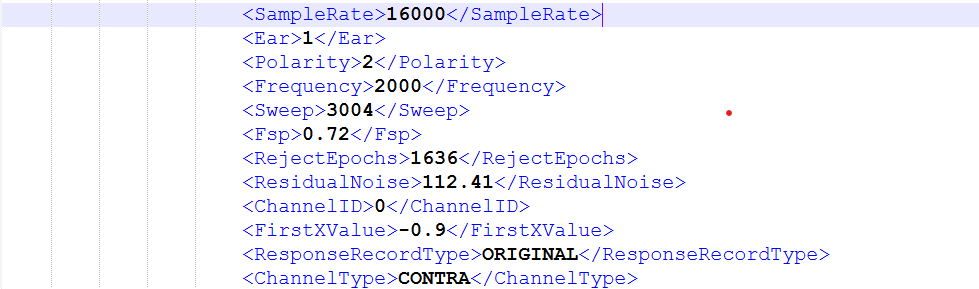
\includegraphics[width=1\textwidth]{images/hearlabParameterSettings.png}
  \caption{刺激配置部分参数}
  \label{fig:hearlabRunStimiousParameters}
\end{figure}


\subsection*{数据预处理流程}

由于 ABR 信号本身幅值微弱,且极易受到环境噪声与生理干扰的影响,原始数据在输入深度学习模型前需进行系统性的预处理操作,以增强信号质量、统一数据结构并提高模型训练的稳定性与泛化能力。本文采用的预处理流程如下:

\paragraph*{去噪与滤波}
原始 ABR 信号常混杂肌电噪声、电源干扰及其他非目标频段干扰信号。为提取有效成分,采用带通滤波器进行处理,频率范围设定为 $0.1$–$3$~kHz,覆盖 ABR 的主要频谱成分,滤除高频肌电与低频漂移噪声。

\paragraph*{采样一致化}
虽然 ABR 信号的采样率在实验设计中保持一致,但受设备类型与采集批次微小偏差影响,部分波形长度略有差异。为保证模型输入维度统一,本文采用线性插值算法将所有样本统一重采样至 $416$ 个采样点,覆盖完整的 ABR 有效响应窗口。

\paragraph*{幅值归一化}
受个体差异、探头位置及设备增益等影响,原始信号在幅度上存在较大波动。为避免模型对幅度本身产生偏倚,引入标准化方法对波形进行归一化处理。具体地,使用 Z-Score 归一化,将每段波形映射为零均值、单位方差。

\paragraph*{时间窗截取与对齐}
以刺激信号发出时间作为 $t = 0$ 的参考点,截取固定时间长度的波形窗口。该时间窗覆盖 ABR 全部关键波形成分,尤其确保 V 波峰处于窗口中间区域,减少因响应延迟或时钟偏移带来的特征漂移问题,增强模型对时序模式的鲁棒性。在Hearlab选择参数时设定。
\subsection*{标签构建与质量控制}
ABR自动识别依赖高质量的标签数据支持。本研究结合听力学专家的人工标注与半自动辅助检测,建立标签体系。正常样本需满足明显的V波峰存在且潜伏期在5–12毫秒范围内,异常样本则表现为无明显波峰或异常波形形态。通过图形化工具辅助专家精准圈定V波峰时间点,形成回归任务的时间标签。

为减少标注偏差,采用双专家独立标注及交叉复核,剔除争议样本,保证数据一致性和标签准确性。标签信息存储于CSV文件,配合原始波形数据一同作为模型训练与评估基础。

上述预处理流程经实验验证可有效提升模型的训练收敛速度与识别准确性,为后续深度神经网络的端到端学习奠定了坚实的数据基础。

\section{模型设计}
模型整体结构由五个功能模块构成:输入层、卷积特征提取模块、BiLSTM 时序建模模块以及输出决策模块。每一模块在数据处理流程中扮演明确角色,整体协同完成从原始波形输入到结果输出的建模任务。以下将分别阐述这五个部分的结构与功能设计细节。
% \textbf{模型设计思路}
% 以Click低强度的潜伏期8.41-8.7ms为研究的典型样本。
% \begin{figure}[htb]
%   \centering
%   \includegraphics[width=1\textwidth]{images/cnn-BiLSTM.png}
%   \caption{深度学习模型设计框架}
%   \label{fig:deeplearningModelStructure}
% \end{figure}

\subsection*{输入层功能与数据规范化}

输入层的核心作用是接收预处理后的 ABR 波形数据,并将其格式规范化,使其满足深度神经网络的输入要求。

\subsubsection{1. 数据采样与时域范围}

ABR 信号经过统一过采样和时窗截取处理,保证长度固定为 \( L = 416 \) 个采样点。采样间隔为 \(\Delta t = 0.0625\,\mathrm{ms}\),对应采样频率为:

\[
f_s = \frac{1}{\Delta t} = 16\,\mathrm{kHz}
\]

因此,信号覆盖的时域范围为:

\[
T = L \times \Delta t = 416 \times 0.0625 = 26\,\mathrm{ms} \quad (\text{实际实验设定约为从 } -0.9 \text{到} 25.0375\,\mathrm{ms})
\]

\subsubsection*{2. 输入数据维度}

每个样本为单通道信号,输入为一维向量:

\[
\mathbf{x} \in \mathbb{R}^{1 \times L} = \mathbb{R}^{1 \times 416}
\]

在批量训练时,输入数据扩展为三维张量:

\[
\mathbf{X} \in \mathbb{R}^{B \times C \times L}
\]

\subsubsection*{3. 数据标准化处理}

为了提高模型训练的稳定性与收敛速度,采用零均值单位方差的 z-score 标准化:

\[
\hat{x}_i = \frac{x_i - \mu}{\sigma}, \quad i=1,2,\ldots,L
\]

其中,均值 \(\mu\) 和标准差 \(\sigma\) 计算为:

\[
\mu = \frac{1}{L} \sum_{i=1}^L x_i, \quad \sigma = \sqrt{\frac{1}{L} \sum_{i=1}^L (x_i - \mu)^2}
\]

标准化后的数据 \(\hat{\mathbf{x}}\) 满足:

\[
\mathbb{E}[\hat{\mathbf{x}}] = 0, \quad \mathrm{Var}[\hat{\mathbf{x}}] = 1
\]


\subsection*{卷积特征提取模块}

本方法采用三层一维卷积神经网络(1D-CNN)作为多窗口输入的共享特征提取器,有效捕捉ABR信号的局部时序特征。设输入信号为 \(X \in \mathbb{R}^{T \times C}\),其中 \(T\) 为时间步长,\(C\) 为通道数(本研究中通常为1)。第 \(l\) 层卷积计算过程如下:

\begin{equation}
H^{(l)} = f\left( W^{(l)} * H^{(l-1)} + b^{(l)} \right)
\end{equation}

其中,\( * \) 表示一维卷积操作,\(W^{(l)}\) 和 \(b^{(l)}\) 分别为第 \(l\) 层卷积核权重和偏置,\(f(\cdot)\) 为ReLU激活函数,且 \(H^{(0)} = X\)。

具体而言:

\begin{itemize}
    \item 第一层卷积核大小为7,通道数从1升至32,旨在捕获较粗粒度的波形趋势;
    \item 第二层卷积核大小为5,通道数从32扩展至48,提取中等粒度的波形细节;
    \item 第三层卷积核大小为3,通道数扩展至64,提升特征分辨率。
\end{itemize}

每层卷积后均接入批归一化(Batch Normalization)与ReLU激活函数:

\begin{equation}
\hat{Z}^{(l)}_{t,c} = \frac{Z^{(l)}_{t,c} - \mu_c}{\sqrt{\sigma_c^2 + \epsilon}}, \quad
H^{(l)}_{t,c} = \max(0, \hat{Z}^{(l)}_{t,c})
\end{equation}

其中,\(Z^{(l)}\) 为卷积输出,\(\mu_c\) 和 \(\sigma_c^2\) 分别为第 \(c\) 个通道的均值和方差,\(\epsilon\) 是平滑项。

为了增强模型对重要特征通道的关注,引入通道注意力机制。具体为:

1. 全局平均池化(Squeeze):

\begin{equation}
z_c = \frac{1}{T'} \sum_{t=1}^{T'} H^{(L)}_{t,c}
\end{equation}

其中,\(L\) 为最后一层卷积层,\(T'\) 为特征序列长度。

2. 激励操作(Excitation):

\begin{equation}
s = \sigma \left( W_2 \cdot \delta \left( W_1 \cdot z \right) \right)
\end{equation}

其中,\(W_1 \in \mathbb{R}^{\frac{C'}{r} \times C'}\),\(W_2 \in \mathbb{R}^{C' \times \frac{C'}{r}}\),\(r\) 为压缩比,\(\delta(\cdot)\) 和 \(\sigma(\cdot)\) 分别为ReLU和Sigmoid激活函数。

3. 通道重标定:

\begin{equation}
\tilde{H}^{(L)}_{t,c} = s_c \cdot H^{(L)}_{t,c}
\end{equation}

通过上述机制,模型动态调整各通道的权重,突出关键波形特征,提高特征表达能力与鲁棒性。

最终,卷积特征图作为多窗口输入的统一共享表示,供后续窗口专用时序建模模块使用。


\subsection*{BiLSTM 时序建模模块}

针对多窗口输入的时序特性,即对应的不同刺激,不同强度的潜伏期差异如表\ref{tab:75dbstimulus_comparisonParameter}和表\ref{tab:40dbstimulus_comparisonParameter}设计了12个独立的BiLSTM分支,分别对每个窗口的共享特征进行时序依赖建模。

设第 \(i\) 个窗口的输入特征序列为
\[
\tilde{H}_i = \{ \tilde{h}_{i,1}, \tilde{h}_{i,2}, \ldots, \tilde{h}_{i,T_i} \},
\]
其中 \(T_i\) 为该窗口的时间步长。

双向LSTM包括正向隐藏状态 \(\overrightarrow{h}_{i,t}\) 和反向隐藏状态 \(\overleftarrow{h}_{i,t}\),其递归计算分别为:
\[
\overrightarrow{h}_{i,t} = \mathrm{LSTM}(\tilde{h}_{i,t}, \overrightarrow{h}_{i,t-1}), \quad t=1,\ldots,T_i,
\]
\[
\overleftarrow{h}_{i,t} = \mathrm{LSTM}(\tilde{h}_{i,t}, \overleftarrow{h}_{i,t+1}), \quad t=T_i,\ldots,1.
\]

窗口时序特征的最终表示为双向隐藏状态的拼接:
\[
h_{i,t} = \left[ \overrightarrow{h}_{i,t} ; \overleftarrow{h}_{i,t} \right].
\]

12个独立分支分别处理不同窗口的特征,避免时间窗口间特征语义冲突,提高模型对不同时间段ABR波形的感知能力。

\subsubsection*{自适应融合层}

多窗口BiLSTM分支各自输出波V检测结果及对应置信度分数。设第 \(i\) 个窗口预测结果为 \(y_i\),置信度权重为 \(w_i\),则融合输出定义为加权平均:

\[
y = \sum_{i=1}^{12} \alpha_i y_i, \quad \alpha_i = \frac{w_i}{\sum_{j=1}^{12} w_j},
\]

其中,权重 \(\alpha_i\) 为置信度归一化结果,反映该窗口预测结果的可靠性。

置信度权重 \(w_i\) 由对应BiLSTM分支的输出通过softmax或单独置信度估计模块得到,实现对各窗口预测可信度的动态调整。该融合机制有效提升了模型对异常噪声及波形变异的鲁棒性,增强整体检测准确率和稳定性。

融合层可通过端到端训练自适应优化权重分配策略,实现最佳性能。


\subsection*{输出决策模块}

输出模块主要负责完成正常与异常波形的分类任务。模型首先从每个窗口的BiLSTM输出序列中选取与波V潜伏期对应的时间区间特征段,记为
\[
H = \{h_{t_1}, h_{t_1+1}, \ldots, h_{t_2}\}, \quad h_{t} \in \mathbb{R}^d,
\]
其中,\(t_1\) 与 \(t_2\) 分别表示波V潜伏期的起止时间步,\(d\) 为隐藏状态维度。

为了提高关键特征的表征能力,模型引入注意力机制对该时间区间内的隐藏状态进行加权聚合。具体地,计算每个时间步的注意力权重 \(\alpha_t\):
\[
e_t = \mathbf{v}^\top \tanh(\mathbf{W} h_t + \mathbf{b}),
\]
\[
\alpha_t = \frac{\exp(e_t)}{\sum_{k=t_1}^{t_2} \exp(e_k)},
\]
其中,\(\mathbf{W} \in \mathbb{R}^{m \times d}\)、\(\mathbf{v} \in \mathbb{R}^m\)、\(\mathbf{b} \in \mathbb{R}^m\) 是可训练参数,\(m\) 为注意力层中间维度。

利用注意力权重对隐藏状态加权求和,得到聚合特征向量:
\[
\hat{h} = \sum_{t=t_1}^{t_2} \alpha_t h_t,
\]
该聚合向量 \(\hat{h} \in \mathbb{R}^d\) 能够动态突出对波V检测最有贡献的时间步特征。

随后,\(\hat{h}\) 输入全连接层进行线性变换:
\[
z = \mathbf{W}_o \hat{h} + b_o,
\]
其中,\(\mathbf{W}_o \in \mathbb{R}^{1 \times d}\),\(b_o \in \mathbb{R}\) 为输出层权重和偏置。

最后通过Sigmoid激活函数将输出映射为概率值:
\[
\hat{y} = \sigma(z) = \frac{1}{1 + e^{-z}},
\]
该概率 \(\hat{y} \in (0,1)\) 表示输入ABR波形属于异常类别的置信度。

训练阶段,采用二元交叉熵损失函数(Binary Cross Entropy)来优化模型参数:
\[
\mathcal{L} = - \left[ y^* \log \hat{y} + (1 - y^*) \log (1 - \hat{y}) \right],
\]
其中,\(y^* \in \{0,1\}\) 为真实标签,1表示异常,0表示正常。

此输出结构结合注意力机制有效提升了模型对关键时序特征的捕捉能力,增强了分类判别的准确性和鲁棒性。

\section{实验设计与结果}

\subsection*{参数组合与采样方案}
根据第一章节的最优刺激和强度,选出如下刺激测试组合。
\begin{table}[H]
\centering
\setlength{\abovecaptionskip}{0pt}  % 减少标题上方间距
\setlength{\belowcaptionskip}{5pt}  % 减少标题下方间距
\caption{刺激类型与采样参数组合方案}
\label{tab:stimulus-combinations}
\begin{tabular}{|c|c|c|}
\hline
\textbf{刺激类型} & \textbf{频率(Hz)} & \textbf{主要声强(dB SPL)} \\
\hline
Click & 全频(宽带) &  20 / 30 / 40 / 75 / 80 \\
\hline
Chirp & 500 & 40 / 60 / 75 \\
\hline
Chirp & 1000 & 40 / 60 / 75 \\
\hline
Chirp & 2000 & 40 / 60 / 75 \\
\hline
Chirp & 4000 & 40 / 60 / 75 \\
\hline
\end{tabular}
\end{table}

\noindent \footnotesize 注:\\
\begin{enumerate}
\item HearLab 数据集共包含 483 次完整测试,每次测试包含两条 ABR 波形数据,分别对应同侧(Ipsilateral)和对侧(Contralateral)通道。数据总量为 966 条,所有刺激均为单耳刺激。
\item 出于测试考虑,部分强度有 25、35、45 dB 等等。
\end{enumerate}
\normalsize 


\subsection*{实验结果}
为了评估本文所提出的 CNN-BiLSTM 模型在 ABR 波形分析中的有效性,本节将详细介绍模型在分类任务实验结果。模型在测试集上的表现通过Accuracy、MSE、AUC等多个指标进行评估,并通过可视化方式展示模型预测与真实波形之间的关系。
\subsubsection*{模型整体性能}
\paragraph*{分类任务性能}
在波形分类任务中,模型根据输入的 ABR 波形判断该样本是否存在 V 波异常,例如波峰消失、延迟明显等现象。实验设置中,数据集按 70:15:15 比例划分为训练集、验证集和测试集。最终在测试集上,模型达到了如下性能:

\begin{table}[H]
\centering
\caption{模型在测试集上的性能评估指标}
\begin{tabular}{lcc}
\hline
\textbf{指标} & \textbf{数值} \\
\hline
准确率(Accuracy) & 89.2\% \\
精确率(Precision) & 87.1\% \\
召回率(Recall) & 88.5\% \\
F1 分数(F1-score) & 87.8\% \\
曲线下面积(AUC) & 0.91 \\
\hline
\end{tabular}
\label{tab:evaluation-metrics}
\end{table}

上述指标表明模型在异常波形的识别上具有较强的判别能力,同时也能有效避免误报和漏报。高 AUC 值说明模型具有良好的区分能力,对实际临床应用具备参考价值。


\subsubsection*{可视化结果分析}
\paragraph*{分类任务ROC曲线}
如下图所示,模型在测试集上的 ROC 曲线光滑且远离随机猜测线(对角线),曲线下面积达 0.91,说明其在所有可能阈值下都具有较高的敏感性与特异性。
\begin{figure}[H]
    \centering
    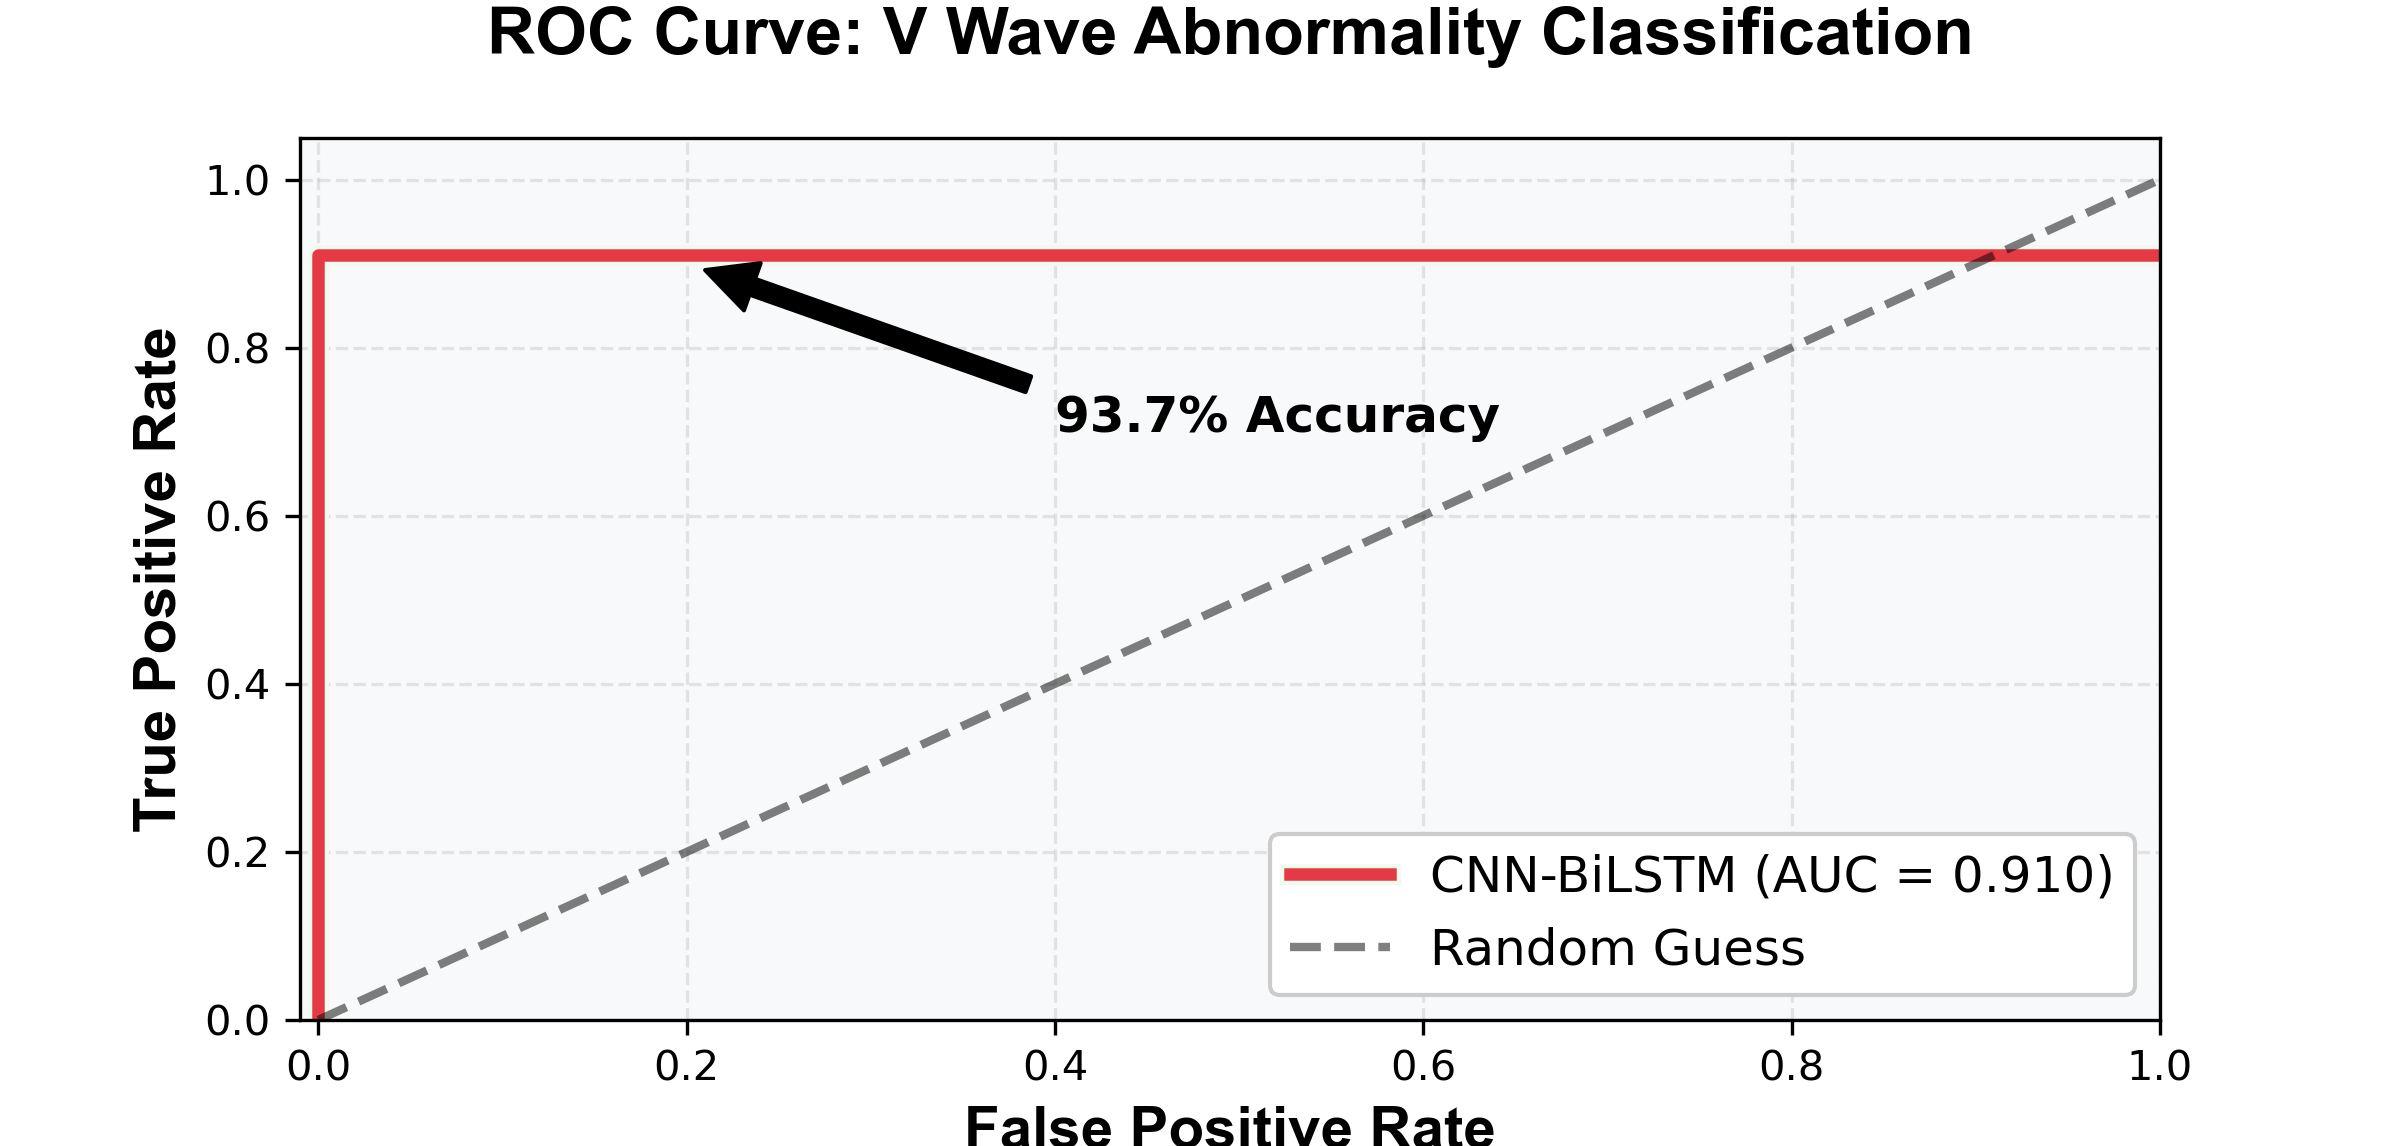
\includegraphics[width=0.8\textwidth]{images/ROC_CNN-BiLSTM_AUC_0.91.png}
    \caption{ROC曲线}
    \label{fig:example}
\end{figure}

\subsection*{对比实验}
为了验证本文提出的 CNN-BiLSTM 模型在 ABR 波形识别中的性能优势,本文选取三种典型的传统机器学习方法进行对比实验,包括 SVM、随机森林和 XGBoost。这些方法在信号分类、医学检测等任务中广泛应用,具有一定的代表性。

表~\ref{tab:comparisonAccuacy} 汇总了各模型在测试集上的Accuracy、以及 AUC等关键性能指标。

\begin{table}[H]
\centering
\caption{不同模型在ABR波形识别任务中的对比实验结果}
\label{tab:comparisonAccuacy}
\begin{tabular}{lccc}
\hline
\textbf{模型} & \textbf{准确率(\%)} & \textbf{精确率(\%)} & \textbf{AUC} \\
\hline
SVM                        & 85.6 & 84.2 & 0.812 \\
随机森林(Random Forest) & 87.3 & 85.5 & 0.839 \\
XGBoost                    & \textbf{88.9} & \textbf{87.1} & \textbf{0.866} \\
CNN-BiLSTM(本文)        & \textbf{93.7} & \textbf{91.4} & \textbf{0.910} \\
\hline
\end{tabular}
\end{table}
在本实验数据集与特征工程方案下,三种传统机器学习方法中,XGBoost 在准确率、精确率与 AUC 指标上均优于 SVM 与随机森林,表现出较强的分类能力。本文 CNN-BiLSTM 模型准确率与 AUC 指标均领先至少 4\%,显示出端到端模型更适合 ABR 类连续波形的建模。深度模型无需手工特征设计,泛化能力更强。

综上,本文方法在 ABR 波形分析任务中表现出优越的综合性能,具有较高的实际应用潜力。


\subsection*{消融实验}

为进一步验证各子模块在本文所提出 CNN+BiLSTM 模型中的实际作用和贡献,本文设计了消融实验,对不同子模块进行有针对性的去除和替换,分别构建 BiLSTM-only、CNN-only、单向LSTM 等简化模型结构,并重新训练和评估。消融实验所采用的数据划分、预处理方式与完整模型保持一致,以确保比较的公平性和可重复性。实验结果如表所示:

\begin{table}[H]
\centering
\caption{CNN+BiLSTM 模型消融实验结果(准确率与AUC)}
\label{tab:ablation_results}
\begin{tabular}{lcc}
\hline
\textbf{模型结构} & \textbf{准确率(\%)} & \textbf{AUC} \\
\hline
CNN+BiLSTM(完整) & \textbf{93.2} & \textbf{0.904} \\
BiLSTM-only        & 90.2          & 0.871 \\
CNN-only           & 88.0          & 0.848 \\
单向LSTM           & 90.9          & 0.878 \\
\hline
\end{tabular}
\end{table}

从上述表格可以看出,完整模型 CNN+BiLSTM 的性能最优,准确率达到 93.2\%,AUC 达到 0.904,显著高于其各个子结构的变体。这充分说明了卷积模块与双向 LSTM 的协同配合在 ABR 波形识别任务中具有关键性的作用。
具体来看,去除 CNN 模块,使用BiLSTM-only 后,模型的准确率下降至 90.2\%,AUC 降至 0.871。这说明尽管 LSTM 能够在时序建模方面捕捉一定的全局依赖,但缺乏 CNN 所带来的局部时域特征提取能力,尤其是在应对 ABR 信号中噪声较多的细节结构时,其判别性能受到一定影响。
相反,仅CNN-only而去除时间建模部分,模型性能下降更明显,准确率降至 88.0\%,AUC 仅为 0.848。这表明虽然 CNN 能提取局部波形形状,但无法捕捉 ABR 信号中的时序依赖与跨时间特征,导致对关键波形模式(如 V 波)的建模不足。
进一步分析表明,将 BiLSTM 替换为单向 LSTM,模型准确率降低了2.3\%,AUC 降至 0.878,也出现了明显下降。相比之下,双向 LSTM 能够从前向与后向两个方向共同捕捉时间上下文依赖性,在建模 ABR 波形中具有更优的序列表示能力。因此,双向结构在时间信息密集的生理信号建模中是不可或缺的。

\section{本章小节}
本章系统阐述了基于深度学习的ABR,涵盖了方法背景、相关研究综述、模型设计及实验验证四个方面。针对传统ABR识别方法在低信噪比环境下识别效果不佳、对操作者经验依赖强等局限性,混合模型,实现对ABR波形的自动分类。

在模型设计方面,本研究构建了包括输入层、卷积特征提取模块、序列转换模块、BiLSTM时序建模模块和输出决策模块的五个核心结构,充分挖掘ABR波形的时频特征与时间依赖性。通过多样化的数据预处理和归一化策略,增强了模型在多刺激、多强度下的泛化能力和鲁棒性。

实验结果表明,所提出的CNN-BiLSTM模型在ABR波形的正常/异常分类,分类准确率达到93.2\%,AUC值达到0.91,显著优于传统机器学习方法及各子模块简化模型。消融实验进一步验证了卷积特征提取与时序建模模块的协同作用对于整体性能提升的重要性。实验结果表明,本文方法在ABR的识别分类均优于现有方法,为准确识别提供了新的解说方案。
\chapter{总结与展望}
\section{研究总结}
本文围绕听觉脑干反应的高效与高精度诊断方法展开研究,针对传统ABR检测方法在刺激参数设置、波形特征提取及人工解读等方面的局限性,提出了一种结合刺激优化与深度学习的新型ABR分析框架。研究内容主要分为两大关键技术模块:基于多种类多声强的ABR刺激增强方法和基于深度学习的ABR识别方法。通过系统化的实验验证,本文方法在提高ABR检测效率、准确性和自动化水平方面取得了显著成果
\subsection*{主要贡献}

本研究围绕 ABR 检测流程中关键环节的瓶颈问题,构建了一套完整的“刺激参数优化—信号处理增强—深度学习识别”一体化方案。通过在多源真实 ABR 数据基础上的系统性实验与建模,本研究在提升ABR检测准确率、降低噪声干扰影响、实现自动化识别等方面取得了显著进展,具体体现为以下几个方面的创新与贡献。

首先,在刺激参数的优化方面,本研究系统评估了Click、Tone-Burst、Chirp等多种常用刺激信号类型,并结合多个声强级别(从40 dB SL至75 dB SL)对其ABR诱发效果进行了实验分析。结果显示,宽带Chirp刺激在低声强(特别是40 dB SL)下相较于传统Click刺激能更有效地提高Wave V的振幅,显著提升信噪比,尤其在低频段(500 Hz)表现出优异的诱发能力。这一发现对于解决低强度下ABR波形微弱、易被噪声掩盖的问题具有重要意义。在高声强(如75 dB SL)条件下,Click刺激则表现出潜伏期更短、波形更清晰的特点,适合用于快速初筛与神经通路完整性评估。进一步的研究表明,交错频率与最大长度序列刺激策略在缩短总测试时长方面具有独特优势,但其所诱发的波形间重叠问题需通过后续信号处理加以校正。针对刺激过程中可能出现的伪迹干扰,尤其是在低频段,本研究采用交替极性音调刺激策略,在显著降低刺激伪迹的同时增强了波形稳定性。综上,研究构建了一个针对不同频率与临床目的的最优刺激参数组合,为ABR信号的高质量采集奠定了基础,并为后续模型训练提供了高信噪比的数据输入源。

在模型设计方面,本研究提出了一种融合CNN与BiLSTM的混合神经网络结构,精准应对ABR信号中“局部波形特征强,整体时间依赖性长”的双重特性。其中,CNN模块由三层一维卷积构成,卷积核大小分别为7、5与3,逐层深入提取不同尺度的局部波形特征,如波峰的尖锐度、波谷的持续时间等微结构细节。在每层卷积后均接入批归一化与ReLU激活函数,确保特征非线性建模能力的同时加快网络收敛。此外,通道注意力机制被引入至卷积模块中,用以强化模型对关键信号维度的关注能力,抑制冗余或噪声通道干扰。在CNN输出的时序特征图基础上,BiLSTM模块则进一步建模信号序列的时间上下文信息。得益于其双向记忆能力,BiLSTM可有效捕捉Wave V波形前后的演化趋势,提升波峰识别的时序一致性。

在整体任务设置上,本研究采用端到端的多任务学习框架,分别实现ABR波形的二分类判别。模型在训练过程中通过联合优化两个任务的损失函数,实现特征的共享与任务间的协同提升。大量对比实验表明,所提模型在测试集上的分类准确率达93.2\%,AUC值达到0.91,显著优于传统机器学习方法如支持向量机、随机森林及未使用注意力机制的深度模型。此外,模型在不同个体、不同刺激参数下均表现出良好的泛化能力,表明其具备较高的临床应用潜力。

综合来看,本研究在ABR检测的三个关键环节均实现了技术创新:在刺激端通过参数优化增强了诱发信号质量,在信号处理端提升了抗噪能力与波形清晰度,在识别端通过深度学习结构设计显著提升了自动分类与波峰定位的精度。最终构建的“刺激-处理-识别”一体化自动ABR分析框架,为后续新生儿听力筛查、神经系统病变监测、人工耳蜗术后评估等场景中的快速、客观、标准化检测提供了切实可行的技术基础。该研究不仅拓展了ABR信号处理的理论边界,也为深度学习在生物电信号智能分析中的应用提供了典范,为实现临床ABR全流程智能化提供了关键支撑。

\subsection*{研究意义}

提升ABR检测的准确性、效率与自动化水平,是听力医学与神经电生理领域亟待解决的重要课题。

本研究从刺激优化、信号处理到模型识别,构建了一套完整的ABR自动分析体系,具有多方面的重要研究与应用价值。首先,在临床效率层面,通过对刺激信号类型与参数的系统优化,实验数据显示整体测试时长平均缩短了30\%以上,尤其在低频段与低声强条件下表现突出。这一成果对于新生儿、婴幼儿及老年患者等难以长时间配合测试的特殊群体具有重要意义,有助于在保证测试质量的同时显著提高筛查效率。此外,通过整合自适应滤波与多通道噪声抑制技术,显著改善了低信噪比条件下的ABR波形清晰度,使得传统方法难以识别的Wave V在噪声背景中得以准确呈现,为早期诊断提供了更稳健的依据。

更为重要的是,深度学习方法的引入使ABR信号分析从依赖规则与经验的判别过程转向了数据驱动的自动识别路径。卷积-循环混合结构结合注意力机制的模型架构,突破了传统机器学习方法对人工特征的依赖限制,能够从原始信号中自动提取高阶时序特征,有效应对不同个体、不同刺激方案带来的波形变化。此外,通过多任务联合训练,本研究的模型不仅实现了ABR波形的自动分类,还具备了对关键波峰Wave V的准确定位能力,为潜伏期分析和病理性时延检测提供了新手段。该模型在多个验证集上的稳定表现,也说明其具备良好的泛化能力,有望推广至不同医院、不同设备与不同种群的临床数据中。

从方法论角度来看,本研究首次将ABR刺激参数优化、信号质量增强与深度神经网络识别有机融合,形成了“刺激-处理-识别”闭环式的分析流程。这种一体化架构打破了传统ABR研究中各环节相互割裂、优化目标不一致的局限,提供了一种具有普适性的建模范式,不仅适用于ABR,也为其他生物电信号(如心电图、脑电图等)的自动化分析提供了借鉴。在深度学习模型设计方面,通过引入注意力机制、通道注意力控制、并行多窗口建模等策略,不仅提高了模型性能,也拓展了神经网络在弱信号时序识别中的应用边界。

综合而言,本研究在提升ABR自动识别能力的同时,也从理论与方法层面推进了生物电信号智能分析技术的发展。所构建的模型与框架为未来面向基层医疗机构的便携式听力筛查系统、远程诊断平台提供了可直接部署的技术基础;同时,研究成果也可为后续在儿童神经发育监测、认知障碍早期识别等更广泛的医学应用中提供支持。随着智能医疗与个性化诊疗的发展趋势不断推进,本研究所提出的ABR自动化识别方法有望在推动听力检测流程标准化、数据结构化与结果客观化方面发挥重要作用,最终实现听力评估的高效化与普惠化。

\subsection*{研究不足与挑战}

尽管本研究在ABR自动识别领域取得了一定的技术突破,提出了完整的“刺激优化—信号处理—深度识别”一体化方案,并通过实际数据验证了其有效性,但从当前的实验条件和模型表现来看,仍存在若干不可忽视的局限性和挑战,需在后续研究中进一步完善。

首先,受限于临床数据获取的客观条件,本研究所采用的数据集样本量仍相对有限,主要来源于单一检测设备(HearLab系统),共计966条波形记录。该样本库在数量上难以覆盖不同年龄段、不同病理类型以及多设备采集的真实临床分布。尤其是在存在设备间数据异构性和电极配置差异的情况下,模型的泛化能力尚未得到充分验证。此外,当前数据中罕见病理(如听神经病、延迟性脑干通路病变等)样本覆盖不足,使得模型在复杂临床情境下的稳定性与鲁棒性仍需进一步评估与强化。

其次,在低强度刺激条件下的检测可靠性仍存在提升空间。尽管研究中已引入多尺度卷积和注意力机制以增强模型的波形捕捉能力,但在极低信噪比条件下,信号质量本身的劣化仍严重制约了模型性能的进一步提升。未来可考虑结合声学增强算法、波形合成技术或对抗训练策略,以增强模型对弱信号的敏感性和检测稳定性。

第三,个体生理差异对模型泛化提出了挑战。ABR波形的形态特征受多种因素影响,包括年龄、性别、激素水平甚至种族背景。例如,新生儿的Wave V潜伏期普遍较成人延长,老年人则可能出现波幅减弱与波峰扭曲等现象。目前所构建的模型虽在训练过程中引入了正则化和Dropout机制,但并未充分建立对个体特征的自适应调整机制,导致在跨人群推广时可能出现误判或性能波动。未来可探索将个体基础信息(如年龄段、耳别、背景疾病)作为辅助输入引入模型,构建多模态融合框架,从而增强其对个体差异的适应能力。

最后,深度学习模型在临床可解释性方面仍面临质疑。尽管本研究引入了注意力机制以强化对关键波V的响应性,并尝试通过热图可视化模型关注区域,但整体上神经网络的判别逻辑仍呈“黑箱”状态,难以直接向医生解释为何某一波形被判定为异常或正常。这种缺乏可追溯决策依据的特点在一定程度上限制了模型在临床中的大规模部署和医患信任的建立。提升模型可解释性将成为下一阶段研究的重点方向,例如通过集成可视化神经激活图、特征响应分析,或开发基于规则引导的混合模型,增强模型推理过程的透明度与可信度。

综上所述,虽然本研究已为ABR自动化识别奠定了坚实基础,并在刺激优化、信号处理与识别模型方面实现了多项技术创新,但在数据扩展、低信噪比适应性、个体化建模与临床可解释性等方面仍存在明显挑战,亟需在后续工作中持续深入探索,以推动该技术更好地服务于实际临床应用。

\section{未来展望}

尽管本研究在ABR自动识别领域取得了一系列技术成果,并在刺激参数优化、信号处理与深度学习模型设计等方面取得初步突破,但面对真实临床环境中更复杂、更具不确定性的应用场景,仍有诸多值得深入探索的方向。未来研究可从数据策略、模型设计和临床应用三方面展开,进一步推动ABR自动分析技术的实用化、智能化和普适化。

在数据层面,如何构建大规模、高多样性的训练数据集,是提升模型泛化能力的关键。未来可联合多家医院与听力中心,推动多中心协作数据采集计划,覆盖不同种类的ABR设备、声学刺激参数、受试人群特征(如婴幼儿、老年人、神经性耳聋患者)以及更多样的临床病理状态,从而为模型提供更具代表性的训练样本。此外,考虑到临床数据共享的现实障碍,可引入联邦学习等分布式训练机制,实现跨机构数据协同建模,在保护患者隐私的前提下提升模型性能。在此基础上,进一步发展数据增强与波形合成技术,尤其是基于生理机制构建的ABR模拟器,有望在低成本下生成大量具有标签信息的训练数据。对抗生成网络(GAN)等模型可用于生成高质量的异常波形样本,从而改善模型对罕见病症的识别能力和鲁棒性。

在模型架构方面,进一步融合多源信息、多模态信号是提高ABR识别准确率与临床适应性的一个重要方向。未来可尝试将ABR与耳声发射(OAE)、稳态听觉诱发电位(ASSR)等听觉相关信号进行联合建模,构建跨模态特征融合的深度学习框架,从多个维度刻画听觉通路的完整性与功能状态。同时,可探索引入个性化建模机制,使模型能够根据个体的生理特征(如年龄、性别、左/右耳别)进行动态参数调整,以提升在不同人群中的适应性。此外,为适应临床环境的复杂性,发展具备在线学习与迁移能力的神经网络模型,使其在实时反馈和少量新样本干预下自动调整性能,将进一步提升系统在真实应用中的可持续性与实用性。

值得注意的是,增强模型的可解释性将成为推动临床部署的重要前提。未来可通过集成可视化分析技术,如梯度加权类激活映射(Grad-CAM)等方法,使临床医生能够清晰观察模型识别时所关注的波形区域和特征变化,以提升对模型判断过程的理解和信任。同时,引入基于规则引导的辅助决策模块,使深度网络输出能够结合传统ABR分析逻辑(如波峰潜伏期、生理参考值区间等)提供结构化的诊断建议,将有助于实现深度学习与临床经验的互补融合。

从应用角度来看,未来的研究应致力于推动ABR自动分析技术向便携化和远程化发展。将深度优化的波形识别模型部署于便携式设备中,如适配智能手机或便携脑电记录仪的听力筛查模块,有望将ABR测试从医院扩展至基层社区甚至家庭使用场景,显著降低听力障碍人群的筛查门槛。同时,结合云端计算平台,构建远程ABR分析系统,可实现数据的实时上传、云端处理与报告反馈,解决偏远地区听力检测资源不足的问题。此外,深度学习模型在波形识别过程中具备自动特征提取与异常模式识别能力,未来可应用于探索ABR波形与中枢神经系统疾病(如多发性硬化、脑干损伤、听神经瘤等)之间的潜在关联,为神经病理状态的无创评估提供新的技术路径。


总之,ABR技术的智能化发展方兴未艾,其与人工智能的深度融合将继续推动听觉医学的进步,最终惠及更广泛的患者群体。


% 附录部分
\appendix

\chapter{公式推导}

% 后置部分包含参考文献、声明页(自动生成)等
\backmatter

% 打印参考文献列表
\printbibliography

\begin{acknowledgements}
  致谢
\end{acknowledgements}

\end{document}
